\chapter{Evaluation -- Images, Figures and Tables}
\label{chapter:appendix-evaluation}

\section{Images}

In addition to the quantitative evaluation of the individual superpixel algorithms in section \ref{section:evaluation-evaluation}, we provide additional material to assess the visual quality of these algorithms with regard to their parameters. For images from the BSDS500, we set the desired number of superpixels to $600$, while for images from the NYUV2 we chose $840$ to be a suitable number of superpixels. For details we refer to the figure captions. Note that, due to space constraints, the algorithms are not sorted as in section \ref{section:evaluation-evaluation}.
\begin{figure}
	\subfigure{
		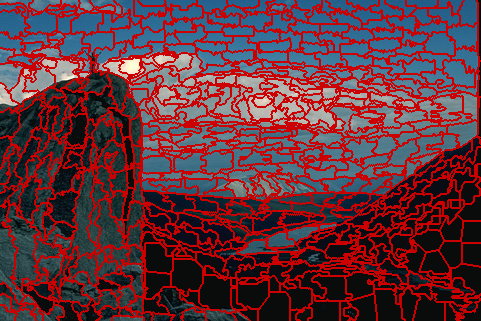
\includegraphics[scale=\scalefivebsd]{pictures/bsd-1-orislic-compactness-005}
	}
	\subfigure{
		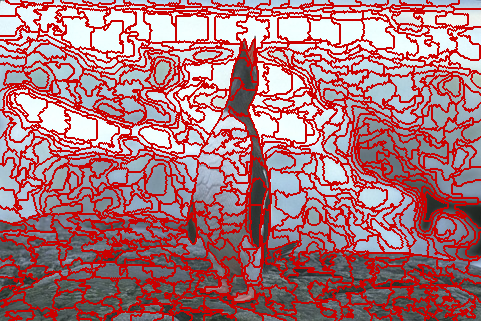
\includegraphics[scale=\scalefivebsd]{pictures/bsd-2-orislic-compactness-005}
	}
	\subfigure{
		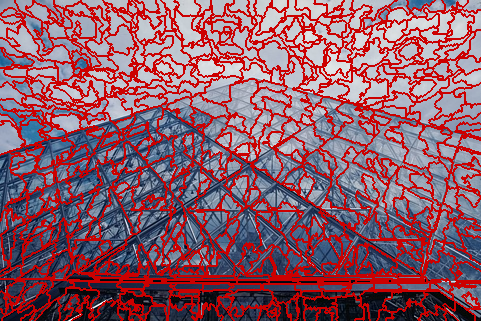
\includegraphics[scale=\scalefivebsd]{pictures/bsd-3-orislic-compactness-005}
	}
	\subfigure{
		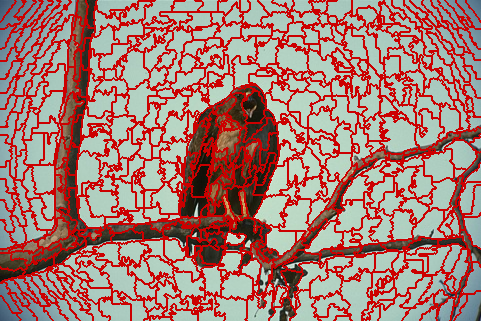
\includegraphics[scale=\scalefivebsd]{pictures/bsd-4-orislic-compactness-005}
	}
	\subfigure{
		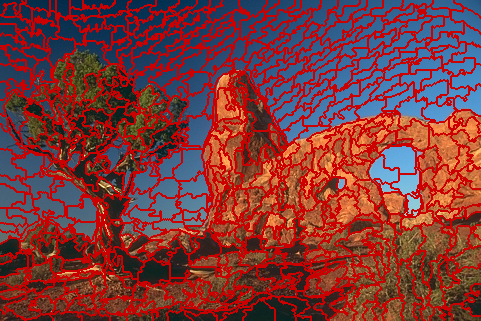
\includegraphics[scale=\scalefivebsd]{pictures/bsd-5-orislic-compactness-005}
	}
	\subfigure{
		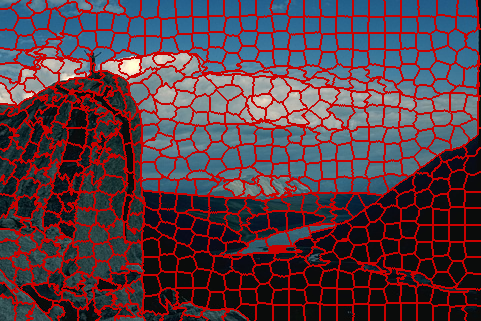
\includegraphics[scale=\scalefivebsd]{pictures/bsd-1-orislic-compactness-10}
	}
	\subfigure{
		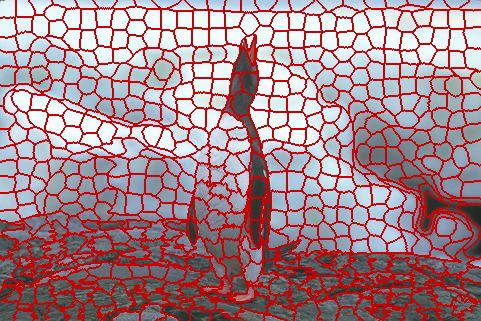
\includegraphics[scale=\scalefivebsd]{pictures/bsd-2-orislic-compactness-10}
	}
	\subfigure{
		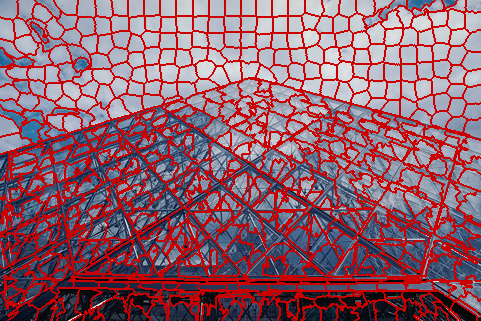
\includegraphics[scale=\scalefivebsd]{pictures/bsd-3-orislic-compactness-10}
	}
	\subfigure{
		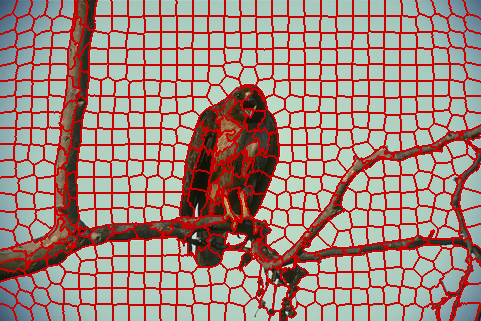
\includegraphics[scale=\scalefivebsd]{pictures/bsd-4-orislic-compactness-10}
	}
	\subfigure{
		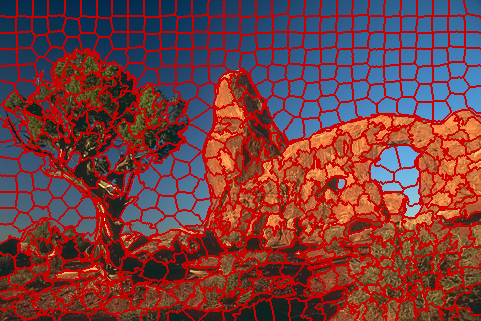
\includegraphics[scale=\scalefivebsd]{pictures/bsd-5-orislic-compactness-10}
	}
	\subfigure{
		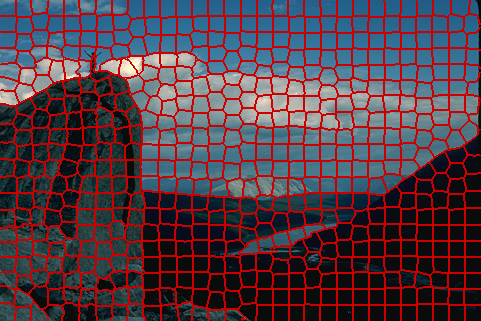
\includegraphics[scale=\scalefivebsd]{pictures/bsd-1-orislic-compactness-40}
	}
	\subfigure{
		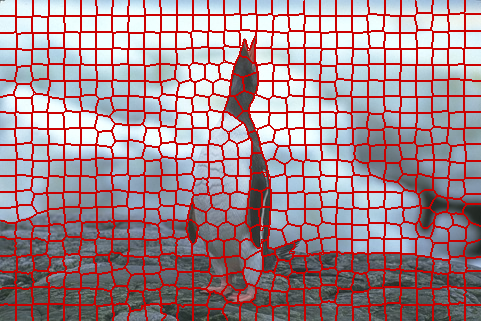
\includegraphics[scale=\scalefivebsd]{pictures/bsd-2-orislic-compactness-40}
	}
	\subfigure{
		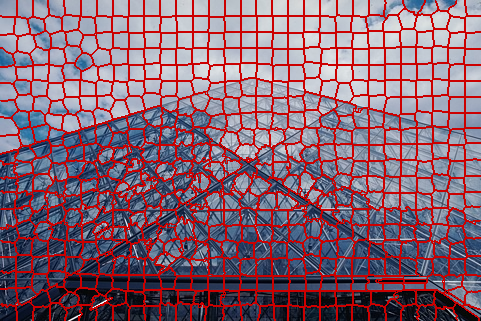
\includegraphics[scale=\scalefivebsd]{pictures/bsd-3-orislic-compactness-40}
	}
	\subfigure{
		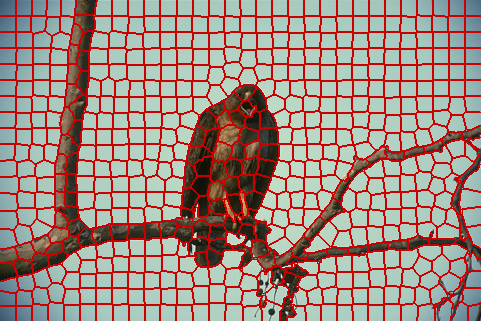
\includegraphics[scale=\scalefivebsd]{pictures/bsd-4-orislic-compactness-40}
	}
	\subfigure{
		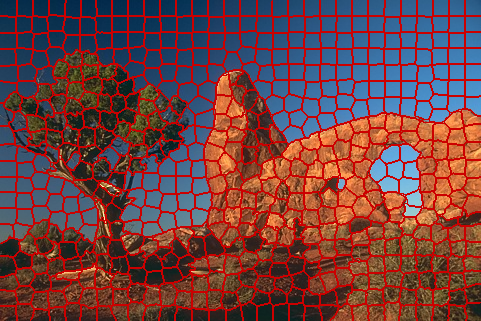
\includegraphics[scale=\scalefivebsd]{pictures/bsd-5-orislic-compactness-40}
	}
	\caption[Qualitative results for the original implementation of \textbf{SLIC} \cite{AchantaShajiSmithLucchiFuaSuesstrunk:2010} illustrating the influence of the compactness parameter $\beta$ on images from the Berkeley Segmentation Dataset \cite{ArbelaezMaireFowlkesMalik:2011}.]{Qualitative results for \textbf{oriSLIC} \cite{AchantaShajiSmithLucchiFuaSuesstrunk:2010} illustrating the influence of the compactness parameter $\beta$ on images from the BSDS500. From top to bottom: $\sqrt{\beta} = 0.05$; $\sqrt{\beta} = 10$ and $\sqrt{\beta} = 40$.}
\end{figure}
\begin{figure}
	\subfigure{
		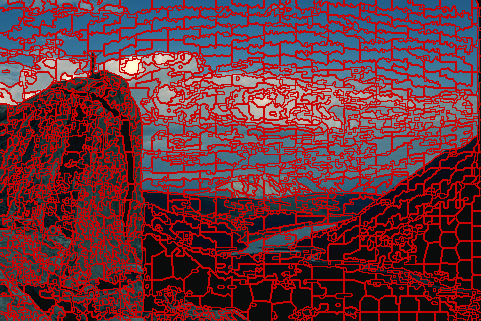
\includegraphics[scale=\scalefivebsd]{{pictures/bsd-1-vlslic-beta-0.5}.png}
	}
	\subfigure{
		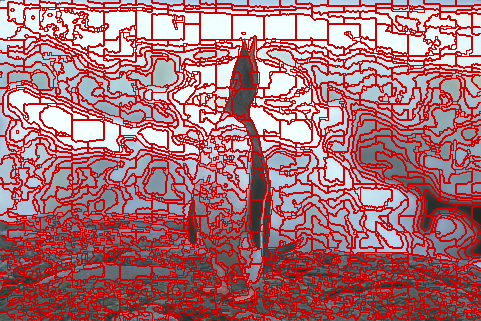
\includegraphics[scale=\scalefivebsd]{{pictures/bsd-2-vlslic-beta-0.5}.png}
	}
	\subfigure{
		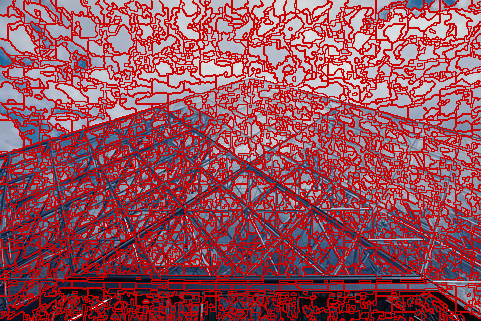
\includegraphics[scale=\scalefivebsd]{{pictures/bsd-3-vlslic-beta-0.5}.png}
	}
	\subfigure{
		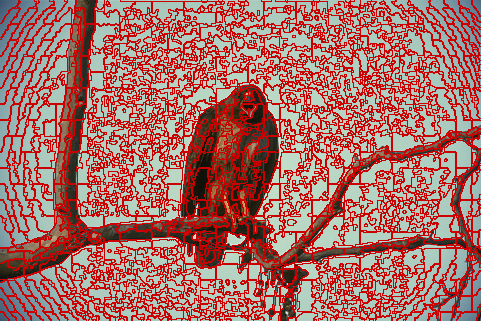
\includegraphics[scale=\scalefivebsd]{{pictures/bsd-4-vlslic-beta-0.5}.png}
	}
	\subfigure{
		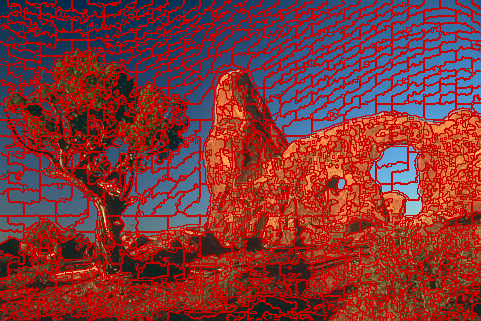
\includegraphics[scale=\scalefivebsd]{{pictures/bsd-5-vlslic-beta-0.5}.png}
	}
	\subfigure{
		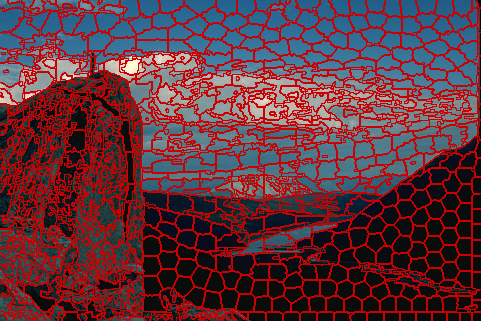
\includegraphics[scale=\scalefivebsd]{{pictures/bsd-1-vlslic-beta-100}.png}
	}
	\subfigure{
		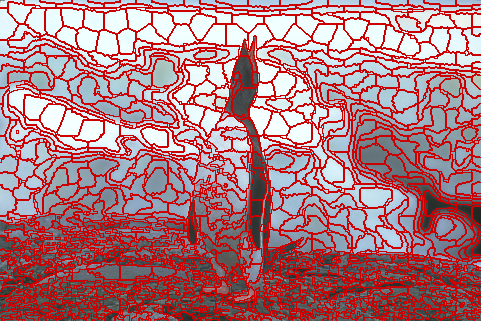
\includegraphics[scale=\scalefivebsd]{{pictures/bsd-2-vlslic-beta-100}.png}
	}
	\subfigure{
		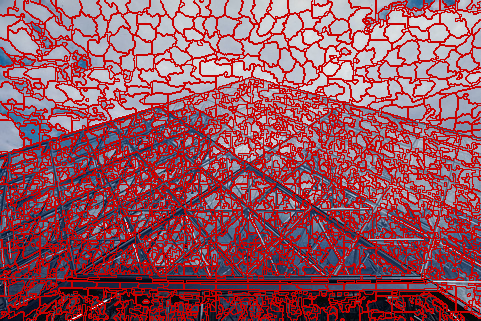
\includegraphics[scale=\scalefivebsd]{{pictures/bsd-3-vlslic-beta-100}.png}
	}
	\subfigure{
		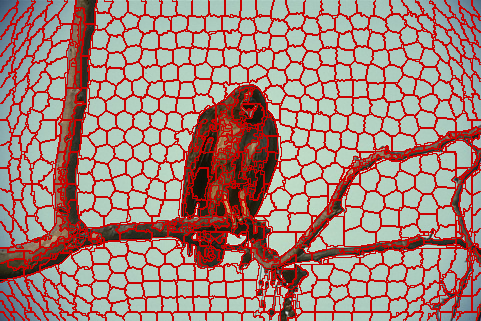
\includegraphics[scale=\scalefivebsd]{{pictures/bsd-4-vlslic-beta-100}.png}
	}
	\subfigure{
		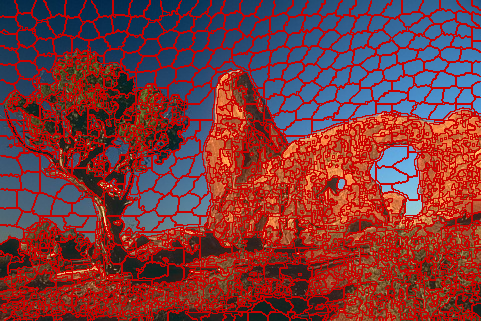
\includegraphics[scale=\scalefivebsd]{{pictures/bsd-5-vlslic-beta-100}.png}
	}
	\caption[Qualitative results for the implementation of \textbf{SLIC} \cite{AchantaShajiSmithLucchiFuaSuesstrunk:2010} provided by the VLFeat Library \cite{VedaldiFulkerson:2008} illustrating the influence of the compactness parameter $\beta$ on images from the Berkeley Segmentation Dataset \cite{ArbelaezMaireFowlkesMalik:2011}.]{Qualitative results for \textbf{vlSLIC} \cite{AchantaShajiSmithLucchiFuaSuesstrunk:2010} illustrating the influence of the compactness parameter $\beta$ on images from the BSDS500. From top to bottom: $\beta = 0.5$ and $\beta = 100$.}
\end{figure}
\begin{figure}
	\subfigure{
		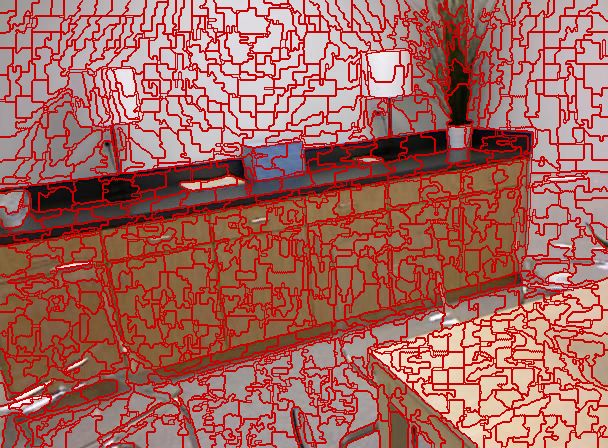
\includegraphics[scale=\scalefivenyu]{pictures/nyu-1-slic3d-beta-005}
	}
	\subfigure{
		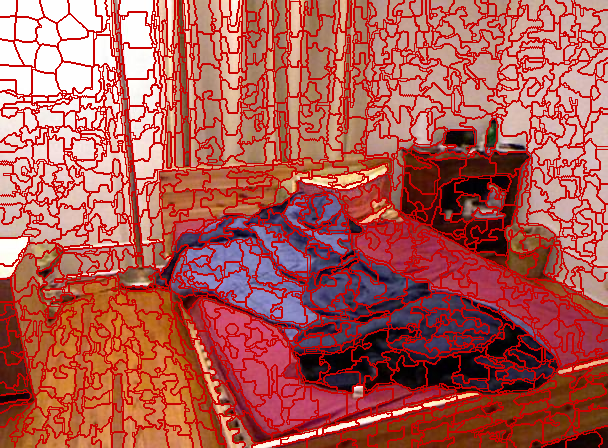
\includegraphics[scale=\scalefivenyu]{pictures/nyu-2-slic3d-beta-005}
	}
	\subfigure{
		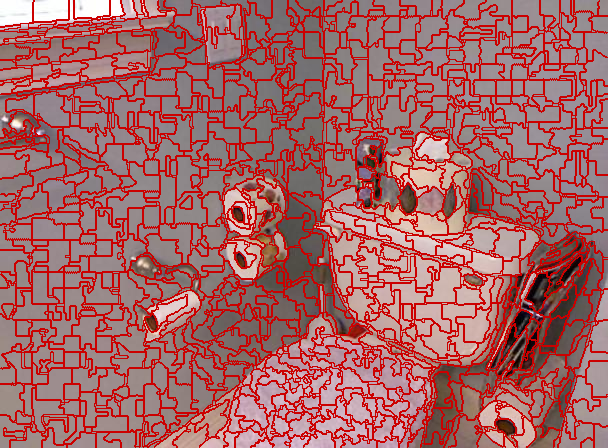
\includegraphics[scale=\scalefivenyu]{pictures/nyu-3-slic3d-beta-005}
	}
	\subfigure{
		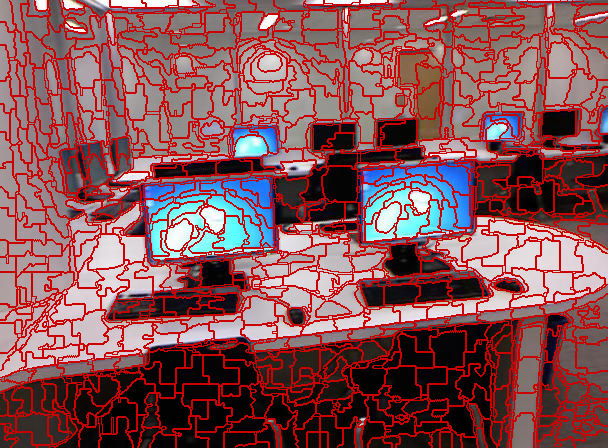
\includegraphics[scale=\scalefivenyu]{pictures/nyu-4-slic3d-beta-005}
	}
	\subfigure{
		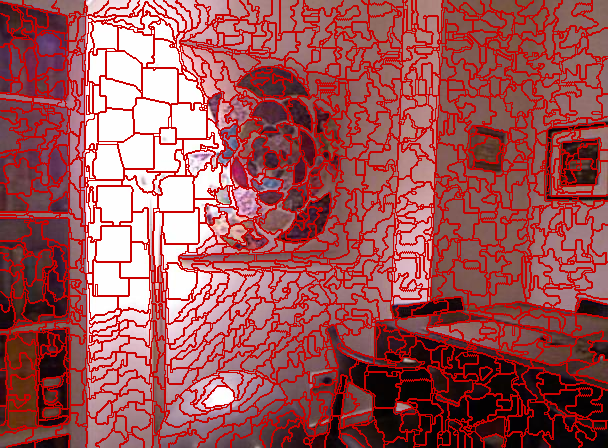
\includegraphics[scale=\scalefivenyu]{pictures/nyu-5-slic3d-beta-005}
	}
	\subfigure{
		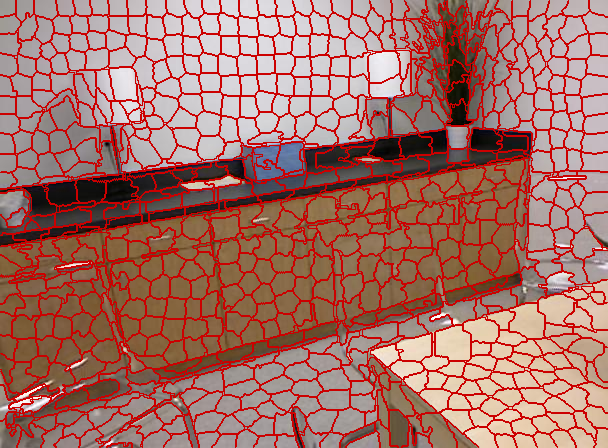
\includegraphics[scale=\scalefivenyu]{pictures/nyu-1-slic3d-beta-10}
	}
	\subfigure{
		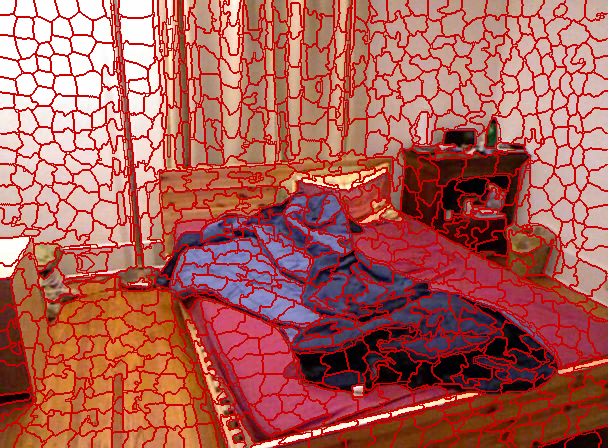
\includegraphics[scale=\scalefivenyu]{pictures/nyu-2-slic3d-beta-10}
	}
	\subfigure{
		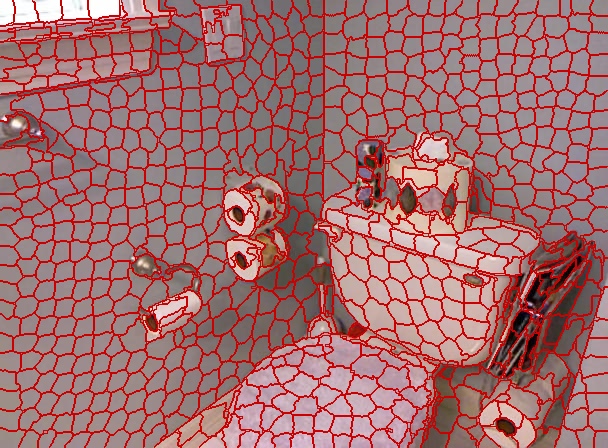
\includegraphics[scale=\scalefivenyu]{pictures/nyu-3-slic3d-beta-10}
	}
	\subfigure{
		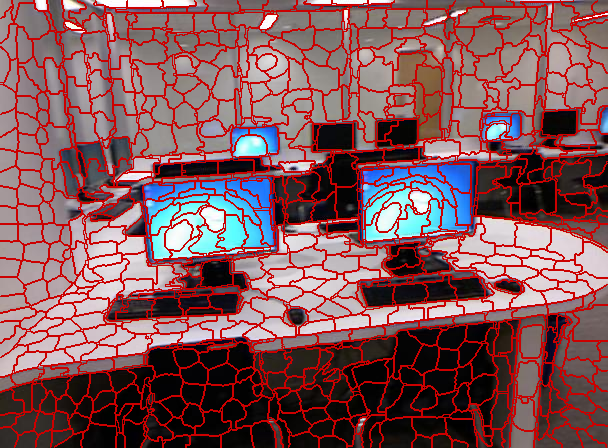
\includegraphics[scale=\scalefivenyu]{pictures/nyu-4-slic3d-beta-10}
	}
	\subfigure{
		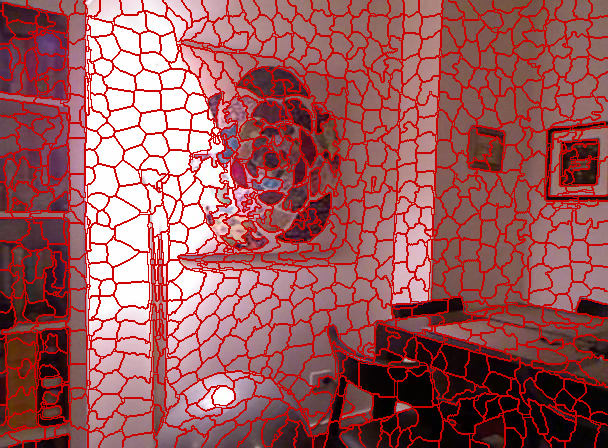
\includegraphics[scale=\scalefivenyu]{pictures/nyu-5-slic3d-beta-10}
	}
	\subfigure{
		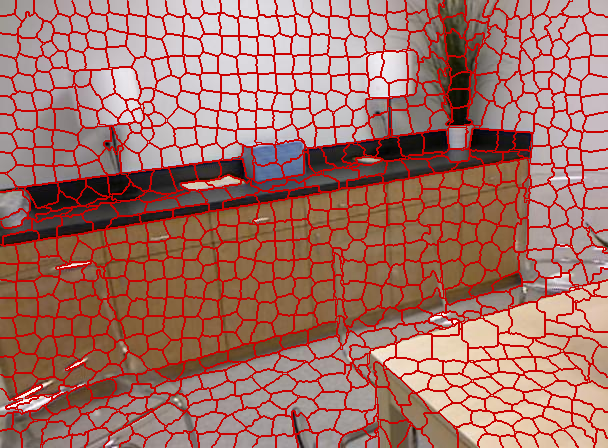
\includegraphics[scale=\scalefivenyu]{pictures/nyu-1-slic3d-beta-40}
	}
	\subfigure{
		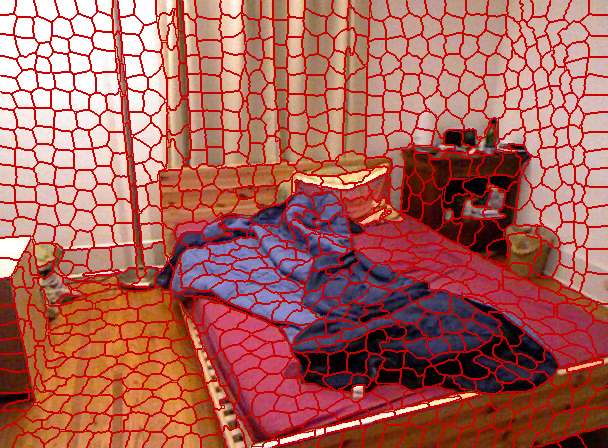
\includegraphics[scale=\scalefivenyu]{pictures/nyu-2-slic3d-beta-40}
	}
	\subfigure{
		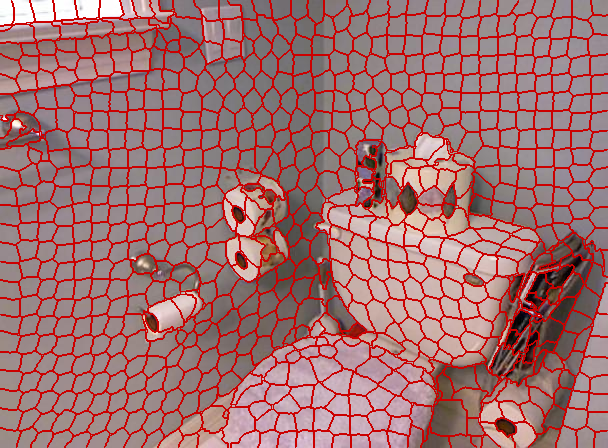
\includegraphics[scale=\scalefivenyu]{pictures/nyu-3-slic3d-beta-40}
	}
	\subfigure{
		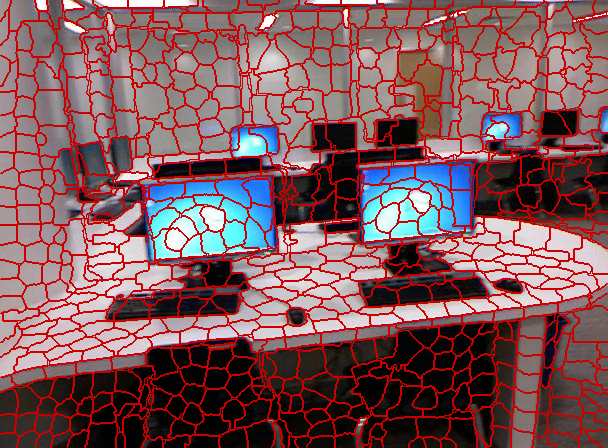
\includegraphics[scale=\scalefivenyu]{pictures/nyu-4-slic3d-beta-40}
	}
	\subfigure{
		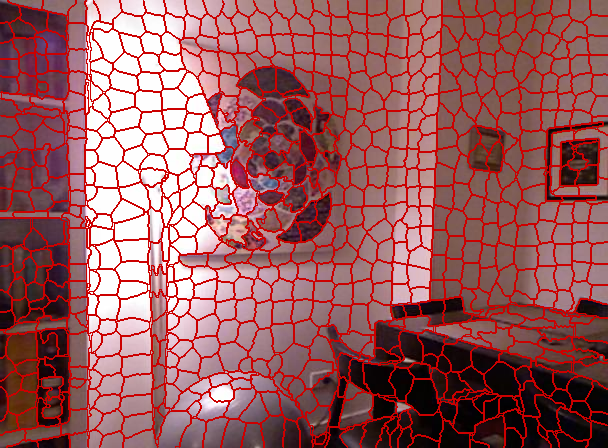
\includegraphics[scale=\scalefivenyu]{pictures/nyu-5-slic3d-beta-40}
	}
	\caption[Qualitative results for \textbf{SLIC3D}, a variant of \textbf{SLIC} \cite{AchantaShajiSmithLucchiFuaSuesstrunk:2010} using depth information, illustrating the influence of the compactness parameter $\beta$ on images from the NYU Depth Dataset \cite{SilbermanHoiemKohliFergus:2012}.]{Qualitative results for \textbf{SLIC3D} illustrating the influence of the compactness parameter $\beta$ on images from the NYUV2. From top to bottom: $\sqrt{\beta} = 0.05$; $\sqrt{\beta} = 10$ and $\sqrt{\beta} = 40$.}
\end{figure}
\begin{figure}
	\subfigure{
		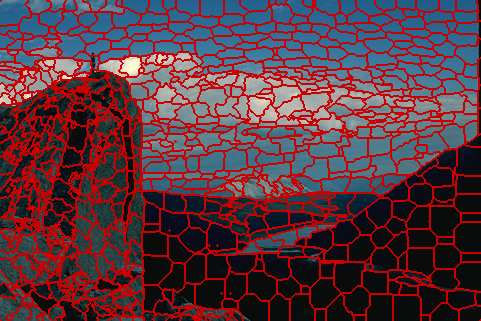
\includegraphics[scale=\scalefivebsd]{pictures/bsd-1-cis-lambda-5}
	}
	\subfigure{
		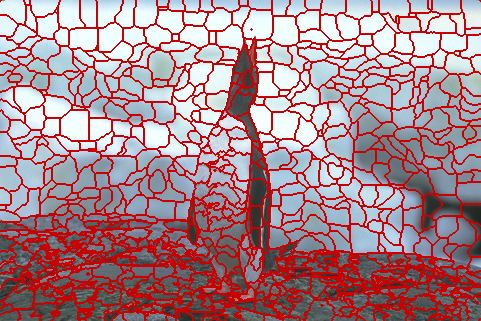
\includegraphics[scale=\scalefivebsd]{pictures/bsd-2-cis-lambda-5}
	}
	\subfigure{
		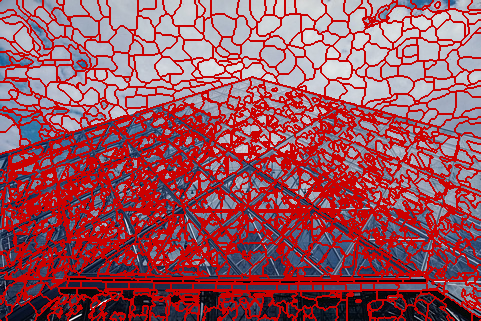
\includegraphics[scale=\scalefivebsd]{pictures/bsd-3-cis-lambda-5}
	}
	\subfigure{
		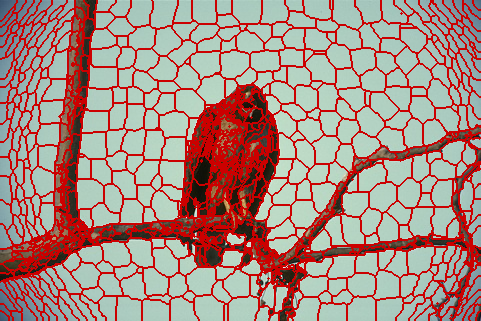
\includegraphics[scale=\scalefivebsd]{pictures/bsd-4-cis-lambda-5}
	}
	\subfigure{
		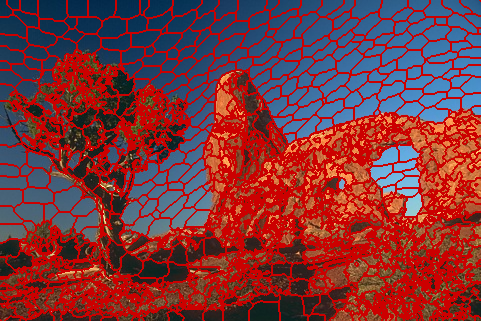
\includegraphics[scale=\scalefivebsd]{pictures/bsd-5-cis-lambda-5}
	}
	\subfigure{
		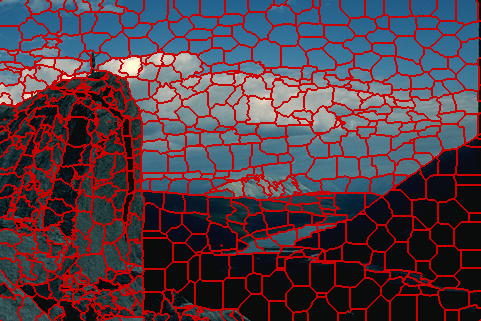
\includegraphics[scale=\scalefivebsd]{pictures/bsd-1-cis-lambda-10}
	}
	\subfigure{
		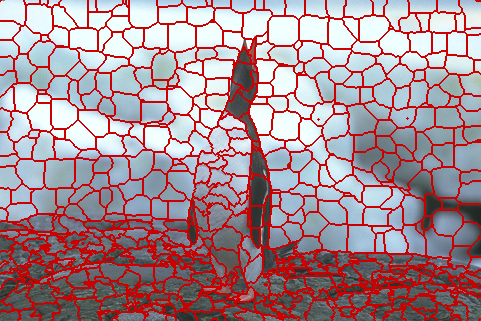
\includegraphics[scale=\scalefivebsd]{pictures/bsd-2-cis-lambda-10}
	}
	\subfigure{
		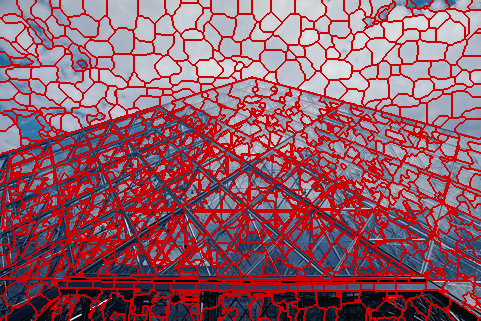
\includegraphics[scale=\scalefivebsd]{pictures/bsd-3-cis-lambda-10}
	}
	\subfigure{
		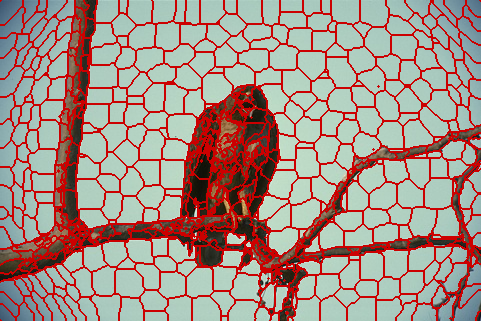
\includegraphics[scale=\scalefivebsd]{pictures/bsd-4-cis-lambda-10}
	}
	\subfigure{
		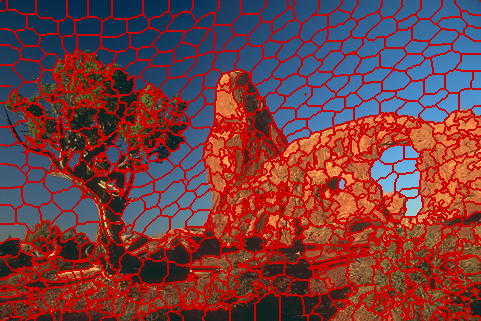
\includegraphics[scale=\scalefivebsd]{pictures/bsd-5-cis-lambda-10}
	}
	\subfigure{
		\includegraphics[scale=\scalefivebsd]{pictures/bsd-1-cis-lambda-25}
	}
	\subfigure{
		\includegraphics[scale=\scalefivebsd]{pictures/bsd-2-cis-lambda-25}
	}
	\subfigure{
		\includegraphics[scale=\scalefivebsd]{pictures/bsd-3-cis-lambda-25}
	}
	\subfigure{
		\includegraphics[scale=\scalefivebsd]{pictures/bsd-4-cis-lambda-25}
	}
	\subfigure{
		\includegraphics[scale=\scalefivebsd]{pictures/bsd-5-cis-lambda-25}
	}
	\caption[Qualitative results for \textbf{CIS} \cite{VekslerBoykovMehrani:2010} illustrating the influence of the parameter $\lambda$ from equation \eqref{eq:related-work-cis-weights} on images from the Berkeley Segmentation Dataset \cite{ArbelaezMaireFowlkesMalik:2011}.]{Qualitative results for \textbf{CIS} \cite{VekslerBoykovMehrani:2010} illustrating the influence of the parameter $\lambda$ from equation \eqref{eq:related-work-cis-weights} on images from the BSDS500. From top to bottom: $\lambda = 5$; $\lambda = 10$ and $\lambda = 25$.}
\end{figure}
\begin{figure}
	\subfigure{
		\includegraphics[scale=\scalefivebsd]{{pictures/bsd-1-ers-lambda-0.2-sigma-4}.png}
	}
	\subfigure{
		\includegraphics[scale=\scalefivebsd]{{pictures/bsd-2-ers-lambda-0.2-sigma-4}.png}
	}
	\subfigure{
		\includegraphics[scale=\scalefivebsd]{{pictures/bsd-3-ers-lambda-0.2-sigma-4}.png}
	}
	\subfigure{
		\includegraphics[scale=\scalefivebsd]{{pictures/bsd-4-ers-lambda-0.2-sigma-4}.png}
	}
	\subfigure{
		\includegraphics[scale=\scalefivebsd]{{pictures/bsd-5-ers-lambda-0.2-sigma-4}.png}
	}
	\subfigure{
		\includegraphics[scale=\scalefivebsd]{{pictures/bsd-1-ers-lambda-0.4-sigma-2}.png}
	}
	\subfigure{
		\includegraphics[scale=\scalefivebsd]{{pictures/bsd-2-ers-lambda-0.4-sigma-2}.png}
	}
	\subfigure{
		\includegraphics[scale=\scalefivebsd]{{pictures/bsd-3-ers-lambda-0.4-sigma-2}.png}
	}
	\subfigure{
		\includegraphics[scale=\scalefivebsd]{{pictures/bsd-4-ers-lambda-0.4-sigma-2}.png}
	}
	\subfigure{
		\includegraphics[scale=\scalefivebsd]{{pictures/bsd-5-ers-lambda-0.4-sigma-2}.png}
	}
	\subfigure{
		\includegraphics[scale=\scalefivebsd]{{pictures/bsd-1-ers-lambda-0.4-sigma-4}.png}
	}
	\subfigure{
		\includegraphics[scale=\scalefivebsd]{{pictures/bsd-2-ers-lambda-0.4-sigma-4}.png}
	}
	\subfigure{
		\includegraphics[scale=\scalefivebsd]{{pictures/bsd-3-ers-lambda-0.4-sigma-4}.png}
	}
	\subfigure{
		\includegraphics[scale=\scalefivebsd]{{pictures/bsd-4-ers-lambda-0.4-sigma-4}.png}
	}
	\subfigure{
		\includegraphics[scale=\scalefivebsd]{{pictures/bsd-5-ers-lambda-0.4-sigma-4}.png}
	}
	\subfigure{
		\includegraphics[scale=\scalefivebsd]{{pictures/bsd-1-ers-lambda-0.4-sigma-6}.png}
	}
	\subfigure{
		\includegraphics[scale=\scalefivebsd]{{pictures/bsd-2-ers-lambda-0.4-sigma-6}.png}
	}
	\subfigure{
		\includegraphics[scale=\scalefivebsd]{{pictures/bsd-3-ers-lambda-0.4-sigma-6}.png}
	}
	\subfigure{
		\includegraphics[scale=\scalefivebsd]{{pictures/bsd-4-ers-lambda-0.4-sigma-6}.png}
	}
	\subfigure{
		\includegraphics[scale=\scalefivebsd]{{pictures/bsd-5-ers-lambda-0.4-sigma-6}.png}
	}
	\subfigure{
		\includegraphics[scale=\scalefivebsd]{{pictures/bsd-1-ers-lambda-0.6-sigma-4}.png}
	}
	\subfigure{
		\includegraphics[scale=\scalefivebsd]{{pictures/bsd-2-ers-lambda-0.6-sigma-4}.png}
	}
	\subfigure{
		\includegraphics[scale=\scalefivebsd]{{pictures/bsd-3-ers-lambda-0.6-sigma-4}.png}
	}
	\subfigure{
		\includegraphics[scale=\scalefivebsd]{{pictures/bsd-4-ers-lambda-0.6-sigma-4}.png}
	}
	\subfigure{
		\includegraphics[scale=\scalefivebsd]{{pictures/bsd-5-ers-lambda-0.6-sigma-4}.png}
	}
	\caption[Qualitative results for \textbf{ERS} \cite{LiuTuzelRamalingamChellappa:2011} illustrating the influence of the parameters $\lambda'$ and $\sigma$, see section \ref{section:evaluation-evaluation}, on images from the Berkeley Segmentation Dataset \cite{ArbelaezMaireFowlkesMalik:2011}.]{Qualitative results for \textbf{ERS} \cite{LiuTuzelRamalingamChellappa:2011} illustrating the influence of the parameters $\lambda'$ and $\sigma$, see section \ref{section:evaluation-evaluation}, on images from the BSDS500. From top to bottom: $\lambda'=0.2$, $\sigma = 4$; $\lambda'=0.4$, $\sigma = 2$; $\lambda'=0.4$, $\sigma = 4$; $\lambda'=0.4$, $\sigma = 6$ and $\lambda'=0.6$, $\sigma = 4$.}
\end{figure}
\begin{figure}
	\subfigure{
		\includegraphics[scale=\scalefivebsd]{pictures/bsd-1-pb-sigma-10}
	}
	\subfigure{
		\includegraphics[scale=\scalefivebsd]{pictures/bsd-2-pb-sigma-10}
	}
	\subfigure{
		\includegraphics[scale=\scalefivebsd]{pictures/bsd-3-pb-sigma-10}
	}
	\subfigure{
		\includegraphics[scale=\scalefivebsd]{pictures/bsd-4-pb-sigma-10}
	}
	\subfigure{
		\includegraphics[scale=\scalefivebsd]{pictures/bsd-5-pb-sigma-10}
	}
	\subfigure{
		\includegraphics[scale=\scalefivebsd]{pictures/bsd-1-pb-sigma-30}
	}
	\subfigure{
		\includegraphics[scale=\scalefivebsd]{pictures/bsd-2-pb-sigma-30}
	}
	\subfigure{
		\includegraphics[scale=\scalefivebsd]{pictures/bsd-3-pb-sigma-30}
	}
	\subfigure{
		\includegraphics[scale=\scalefivebsd]{pictures/bsd-4-pb-sigma-30}
	}
	\subfigure{
		\includegraphics[scale=\scalefivebsd]{pictures/bsd-5-pb-sigma-30}
	}
	\subfigure{
		\includegraphics[scale=\scalefivebsd]{pictures/bsd-1-pb-sigma-50}
	}
	\subfigure{
		\includegraphics[scale=\scalefivebsd]{pictures/bsd-2-pb-sigma-50}
	}
	\subfigure{
		\includegraphics[scale=\scalefivebsd]{pictures/bsd-3-pb-sigma-50}
	}
	\subfigure{
		\includegraphics[scale=\scalefivebsd]{pictures/bsd-4-pb-sigma-50}
	}
	\subfigure{
		\includegraphics[scale=\scalefivebsd]{pictures/bsd-5-pb-sigma-50}
	}
	\caption[Qualitative results for \textbf{PB} \cite{ZhangHartleyMashfordBurn:2011} illustrating the influence of the parameter $\sigma$ on images from the Berkeley Segmentation Dataset \cite{ArbelaezMaireFowlkesMalik:2011}.]{Qualitative results for \textbf{PB} \cite{ZhangHartleyMashfordBurn:2011} illustrating the influence of the parameter $\sigma$ on images from the BSDS500. From top to bottom: $\sigma = 10$; $\sigma = 30$ and $\sigma = 50$.}
\end{figure}
\begin{figure}
	\subfigure{
		\includegraphics[scale=\scalefivebsd]{pictures/bsd-1-crs-compactness-0005}
	}
	\subfigure{
		\includegraphics[scale=\scalefivebsd]{pictures/bsd-2-crs-compactness-0005}
	}
	\subfigure{
		\includegraphics[scale=\scalefivebsd]{pictures/bsd-3-crs-compactness-0005}
	}
	\subfigure{
		\includegraphics[scale=\scalefivebsd]{pictures/bsd-4-crs-compactness-0005}
	}
	\subfigure{
		\includegraphics[scale=\scalefivebsd]{pictures/bsd-5-crs-compactness-0005}
	}
	\subfigure{
		\includegraphics[scale=\scalefivebsd]{pictures/bsd-1-crs-compactness-005}
	}
	\subfigure{
		\includegraphics[scale=\scalefivebsd]{pictures/bsd-2-crs-compactness-005}
	}
	\subfigure{
		\includegraphics[scale=\scalefivebsd]{pictures/bsd-3-crs-compactness-005}
	}
	\subfigure{
		\includegraphics[scale=\scalefivebsd]{pictures/bsd-4-crs-compactness-005}
	}
	\subfigure{
		\includegraphics[scale=\scalefivebsd]{pictures/bsd-5-crs-compactness-005}
	}
	\subfigure{
		\includegraphics[scale=\scalefivebsd]{pictures/bsd-1-crs-compactness-02}
	}
	\subfigure{
		\includegraphics[scale=\scalefivebsd]{pictures/bsd-2-crs-compactness-02}
	}
	\subfigure{
		\includegraphics[scale=\scalefivebsd]{pictures/bsd-3-crs-compactness-02}
	}
	\subfigure{
		\includegraphics[scale=\scalefivebsd]{pictures/bsd-4-crs-compactness-02}
	}
	\subfigure{
		\includegraphics[scale=\scalefivebsd]{pictures/bsd-5-crs-compactness-02}
	}
	\caption[Qualitative results for \textbf{CRS} \cite{ConradMertzMester:2013} illustrating the influence of the compactness parameter $\beta$ on images from the Berkeley Segmentation Dataset \cite{ArbelaezMaireFowlkesMalik:2011}.]{Qualitative results for \textbf{CRS} \cite{ConradMertzMester:2013} illustrating the influence of the compactness parameter $\beta$ on images from the BSDS500. From top to bottom: $\beta = 0.005$; $\beta = 0.05$ and $\beta = 0.2$.}
\end{figure}
\begin{figure}
	\subfigure{
		\includegraphics[scale=\scalefivebsd]{pictures/bsd-1-oriseeds}
	}
	\subfigure{
		\includegraphics[scale=\scalefivebsd]{pictures/bsd-2-oriseeds}
	}
	\subfigure{
		\includegraphics[scale=\scalefivebsd]{pictures/bsd-3-oriseeds}
	}
	\subfigure{
		\includegraphics[scale=\scalefivebsd]{pictures/bsd-4-oriseeds}
	}
	\subfigure{
		\includegraphics[scale=\scalefivebsd]{pictures/bsd-5-oriseeds}
	}
	\subfigure{
		\includegraphics[scale=\scalefivebsd]{pictures/bsd-1-oriseedsmp}
	}
	\subfigure{
		\includegraphics[scale=\scalefivebsd]{pictures/bsd-2-oriseedsmp}
	}
	\subfigure{
		\includegraphics[scale=\scalefivebsd]{pictures/bsd-3-oriseedsmp}
	}
	\subfigure{
		\includegraphics[scale=\scalefivebsd]{pictures/bsd-4-oriseedsmp}
	}
	\subfigure{
		\includegraphics[scale=\scalefivebsd]{pictures/bsd-5-oriseedsmp}
	}
	\subfigure{
		\includegraphics[scale=\scalefivebsd]{pictures/bsd-1-reseeds-neighborhood-0}
	}
	\subfigure{
		\includegraphics[scale=\scalefivebsd]{pictures/bsd-2-reseeds-neighborhood-0}
	}
	\subfigure{
		\includegraphics[scale=\scalefivebsd]{pictures/bsd-3-reseeds-neighborhood-0}
	}
	\subfigure{
		\includegraphics[scale=\scalefivebsd]{pictures/bsd-4-reseeds-neighborhood-0}
	}
	\subfigure{
		\includegraphics[scale=\scalefivebsd]{pictures/bsd-5-reseeds-neighborhood-0}
	}
	\subfigure{
		\includegraphics[scale=\scalefivebsd]{pictures/bsd-1-reseeds-neighborhood-1}
	}
	\subfigure{
		\includegraphics[scale=\scalefivebsd]{pictures/bsd-2-reseeds-neighborhood-1}
	}
	\subfigure{
		\includegraphics[scale=\scalefivebsd]{pictures/bsd-3-reseeds-neighborhood-1}
	}
	\subfigure{
		\includegraphics[scale=\scalefivebsd]{pictures/bsd-4-reseeds-neighborhood-1}
	}
	\subfigure{
		\includegraphics[scale=\scalefivebsd]{pictures/bsd-5-reseeds-neighborhood-1}
	}
	\subfigure{
		\includegraphics[scale=\scalefivebsd]{pictures/bsd-1-reseedsmp-bins-5}
	}
	\subfigure{
		\includegraphics[scale=\scalefivebsd]{pictures/bsd-2-reseedsmp-bins-5}
	}
	\subfigure{
		\includegraphics[scale=\scalefivebsd]{pictures/bsd-3-reseedsmp-bins-5}
	}
	\subfigure{
		\includegraphics[scale=\scalefivebsd]{pictures/bsd-4-reseedsmp-bins-5}
	}
	\subfigure{
		\includegraphics[scale=\scalefivebsd]{pictures/bsd-5-reseedsmp-bins-5}
	}
	\subfigure{
		\includegraphics[scale=\scalefivebsd]{pictures/bsd-1-reseedsmp}
	}
	\subfigure{
		\includegraphics[scale=\scalefivebsd]{pictures/bsd-2-reseedsmp}
	}
	\subfigure{
		\includegraphics[scale=\scalefivebsd]{pictures/bsd-3-reseedsmp}
	}
	\subfigure{
		\includegraphics[scale=\scalefivebsd]{pictures/bsd-4-reseedsmp}
	}
	\subfigure{
		\includegraphics[scale=\scalefivebsd]{pictures/bsd-5-reseedsmp}
	}
	\subfigure{
		\includegraphics[scale=\scalefivebsd]{{pictures/bsd-1-reseedssm-beta-0.25}.png}
	}
	\subfigure{
		\includegraphics[scale=\scalefivebsd]{{pictures/bsd-2-reseedssm-beta-0.25}.png}
	}
	\subfigure{
		\includegraphics[scale=\scalefivebsd]{{pictures/bsd-3-reseedssm-beta-0.25}.png}
	}
	\subfigure{
		\includegraphics[scale=\scalefivebsd]{{pictures/bsd-4-reseedssm-beta-0.25}.png}
	}
	\subfigure{
		\includegraphics[scale=\scalefivebsd]{{pictures/bsd-5-reseedssm-beta-0.25}.png}
	}
	\subfigure{
		\includegraphics[scale=\scalefivebsd]{{pictures/bsd-1-reseedssm-beta-0.75}.png}
	}
	\subfigure{
		\includegraphics[scale=\scalefivebsd]{{pictures/bsd-2-reseedssm-beta-0.75}.png}
	}
	\subfigure{
		\includegraphics[scale=\scalefivebsd]{{pictures/bsd-3-reseedssm-beta-0.75}.png}
	}
	\subfigure{
		\includegraphics[scale=\scalefivebsd]{{pictures/bsd-4-reseedssm-beta-0.75}.png}
	}
	\subfigure{
		\includegraphics[scale=\scalefivebsd]{{pictures/bsd-5-reseedssm-beta-0.75}.png}
	}
	\caption[Qualitative results for the original implementation of \textbf{SEEDS} \cite{VanDenBerghBoixRoigCapitaniVanGool:2012} and our implementation of \textbf{SEEDS} illustrating the influence of the smoothing term of equation \eqref{eq:superpixle-segmentation-seeds-original-smoothing}, mean pixel updates and the histogram size $Q$ on images from the Berkeley Segmentation Dataset \cite{ArbelaezMaireFowlkesMalik:2011}.]{Qualitative results for \textbf{oriSEEDS} \cite{VanDenBerghBoixRoigCapitaniVanGool:2012} and \textbf{reSEEDS} illustrating the influence of the smoothing term of equation \eqref{eq:superpixle-segmentation-seeds-original-smoothing}, mean pixel updates and the histogram size $Q$ on images from the BSDS500. When not noted differently, results were obtained using the smoothing term of equation \eqref{eq:superpixle-segmentation-seeds-original-smoothing} and $Q = 7^3$ as well as $T = 2$. For details refer to the discussion in section \ref{section:evaluation-evaluation}. From top to bottom: \textbf{oriSEEDS}; \textbf{oriSEEDSmp}; \textbf{reSEEDS} without smoothing term; \textbf{reSEEDS}; \textbf{reSEEDSmp}, $Q = 5^3$; \textbf{reSEEDSmp}, $Q = 7^3$; \textbf{reSEEDSmp*}, $\beta = 0.25$ and \textbf{reSEEDSmp*}, $\beta = 0.75$.}
\end{figure}
\begin{figure}
	\subfigure{
		\includegraphics[scale=\scalefivenyu]{{pictures/nyu-1-seeds3d-beta-0.5}.png}
	}
	\subfigure{
		\includegraphics[scale=\scalefivenyu]{{pictures/nyu-2-seeds3d-beta-0.5}.png}
	}
	\subfigure{
		\includegraphics[scale=\scalefivenyu]{{pictures/nyu-3-seeds3d-beta-0.5}.png}
	}
	\subfigure{
		\includegraphics[scale=\scalefivenyu]{{pictures/nyu-4-seeds3d-beta-0.5}.png}
	}
	\subfigure{
		\includegraphics[scale=\scalefivenyu]{{pictures/nyu-5-seeds3d-beta-0.5}.png}
	}
	\subfigure{
		\includegraphics[scale=\scalefivenyu]{{pictures/nyu-1-seeds3d-beta-1}.png}
	}
	\subfigure{
		\includegraphics[scale=\scalefivenyu]{{pictures/nyu-2-seeds3d-beta-1}.png}
	}
	\subfigure{
		\includegraphics[scale=\scalefivenyu]{{pictures/nyu-3-seeds3d-beta-1}.png}
	}
	\subfigure{
		\includegraphics[scale=\scalefivenyu]{{pictures/nyu-4-seeds3d-beta-1}.png}
	}
	\subfigure{
		\includegraphics[scale=\scalefivenyu]{{pictures/nyu-5-seeds3d-beta-1}.png}
	}
	\subfigure{
		\includegraphics[scale=\scalefivenyu]{{pictures/nyu-1-seeds3d-beta-1.5}.png}
	}
	\subfigure{
		\includegraphics[scale=\scalefivenyu]{{pictures/nyu-2-seeds3d-beta-1.5}.png}
	}
	\subfigure{
		\includegraphics[scale=\scalefivenyu]{{pictures/nyu-3-seeds3d-beta-1.5}.png}
	}
	\subfigure{
		\includegraphics[scale=\scalefivenyu]{{pictures/nyu-4-seeds3d-beta-1.5}.png}
	}
	\subfigure{
		\includegraphics[scale=\scalefivenyu]{{pictures/nyu-5-seeds3d-beta-1.5}.png}
	}
	\subfigure{
		\includegraphics[scale=\scalefivenyu]{{pictures/nyu-1-seeds3dn-beta-0.5-gamma-0.005}.png}
	}
	\subfigure{
		\includegraphics[scale=\scalefivenyu]{{pictures/nyu-2-seeds3dn-beta-0.5-gamma-0.005}.png}
	}
	\subfigure{
		\includegraphics[scale=\scalefivenyu]{{pictures/nyu-3-seeds3dn-beta-0.5-gamma-0.005}.png}
	}
	\subfigure{
		\includegraphics[scale=\scalefivenyu]{{pictures/nyu-4-seeds3dn-beta-0.5-gamma-0.005}.png}
	}
	\subfigure{
		\includegraphics[scale=\scalefivenyu]{{pictures/nyu-5-seeds3dn-beta-0.5-gamma-0.005}.png}
	}
	\subfigure{
		\includegraphics[scale=\scalefivenyu]{{pictures/nyu-1-seeds3dn-beta-0.5-gamma-0.1}.png}
	}
	\subfigure{
		\includegraphics[scale=\scalefivenyu]{{pictures/nyu-2-seeds3dn-beta-0.5-gamma-0.1}.png}
	}
	\subfigure{
		\includegraphics[scale=\scalefivenyu]{{pictures/nyu-3-seeds3dn-beta-0.5-gamma-0.1}.png}
	}
	\subfigure{
		\includegraphics[scale=\scalefivenyu]{{pictures/nyu-4-seeds3dn-beta-0.5-gamma-0.1}.png}
	}
	\subfigure{
		\includegraphics[scale=\scalefivenyu]{{pictures/nyu-5-seeds3dn-beta-0.5-gamma-0.1}.png}
	}
	\subfigure{
		\includegraphics[scale=\scalefivenyu]{{pictures/nyu-1-seeds3dn-beta-0.5-gamma-0.25}.png}
	}
	\subfigure{
		\includegraphics[scale=\scalefivenyu]{{pictures/nyu-2-seeds3dn-beta-0.5-gamma-0.25}.png}
	}
	\subfigure{
		\includegraphics[scale=\scalefivenyu]{{pictures/nyu-3-seeds3dn-beta-0.5-gamma-0.25}.png}
	}
	\subfigure{
		\includegraphics[scale=\scalefivenyu]{{pictures/nyu-4-seeds3dn-beta-0.5-gamma-0.25}.png}
	}
	\subfigure{
		\includegraphics[scale=\scalefivenyu]{{pictures/nyu-5-seeds3dn-beta-0.5-gamma-0.25}.png}
	}
	\caption[Qualitative results for the extension of \textbf{SEEDS} \cite{VanDenBerghBoixRoigCapitaniVanGool:2012} using 3D point coordinates and normal information for pixel updates illustrated on images from the NYU Depth Dataset \cite{SilbermanHoiemKohliFergus:2012}.]{Qualitative results for \textbf{SEEDS3D} and \textbf{SEEDS3Dn} illustrating the influence of the parameters $\beta$ and $\gamma$ on images from the NYUV2. From top to bottom: \textbf{SEEDS3D} with $\beta = 0.5$; \textbf{SEEDS3D} with $\beta = 1$; \textbf{SEEDS3D} with $\beta = 1.5$; \textbf{SEEDS3Dn} with $\beta = 0.5$ and $\gamma = 0.005$; \textbf{SEEDS3Dn} with $\beta = 0.5$ and $\gamma = 0.1$ and \textbf{SEEDS3Dn} with $\beta = 0.5$ and $\gamma = 0.25$}
\end{figure}
\begin{figure}
	\subfigure{
		\includegraphics[scale=\scalefivenyu]{{pictures/nyu-1-dasp-beta-0-gamma-0}.png}
	}
	\subfigure{
		\includegraphics[scale=\scalefivenyu]{{pictures/nyu-2-dasp-beta-0-gamma-0}.png}
	}
	\subfigure{
		\includegraphics[scale=\scalefivenyu]{{pictures/nyu-3-dasp-beta-0-gamma-0}.png}
	}
	\subfigure{
		\includegraphics[scale=\scalefivenyu]{{pictures/nyu-4-dasp-beta-0-gamma-0}.png}
	}
	\subfigure{
		\includegraphics[scale=\scalefivenyu]{{pictures/nyu-5-dasp-beta-0-gamma-0}.png}
	}
	\subfigure{
		\includegraphics[scale=\scalefivenyu]{{pictures/nyu-1-dasp-beta-0.05-gamma-0}.png}
	}
	\subfigure{
		\includegraphics[scale=\scalefivenyu]{{pictures/nyu-2-dasp-beta-0.05-gamma-0}.png}
	}
	\subfigure{
		\includegraphics[scale=\scalefivenyu]{{pictures/nyu-3-dasp-beta-0.05-gamma-0}.png}
	}
	\subfigure{
		\includegraphics[scale=\scalefivenyu]{{pictures/nyu-4-dasp-beta-0.05-gamma-0}.png}
	}
	\subfigure{
		\includegraphics[scale=\scalefivenyu]{{pictures/nyu-5-dasp-beta-0.05-gamma-0}.png}
	}
	\subfigure{
		\includegraphics[scale=\scalefivenyu]{{pictures/nyu-1-dasp-beta-0.25-gamma-0}.png}
	}
	\subfigure{
		\includegraphics[scale=\scalefivenyu]{{pictures/nyu-2-dasp-beta-0.25-gamma-0}.png}
	}
	\subfigure{
		\includegraphics[scale=\scalefivenyu]{{pictures/nyu-3-dasp-beta-0.25-gamma-0}.png}
	}
	\subfigure{
		\includegraphics[scale=\scalefivenyu]{{pictures/nyu-4-dasp-beta-0.25-gamma-0}.png}
	}
	\subfigure{
		\includegraphics[scale=\scalefivenyu]{{pictures/nyu-5-dasp-beta-0.25-gamma-0}.png}
	}
	\subfigure{
		\includegraphics[scale=\scalefivenyu]{{pictures/nyu-1-dasp-beta-0-gamma-1.5}.png}
	}
	\subfigure{
		\includegraphics[scale=\scalefivenyu]{{pictures/nyu-2-dasp-beta-0-gamma-1.5}.png}
	}
	\subfigure{
		\includegraphics[scale=\scalefivenyu]{{pictures/nyu-3-dasp-beta-0-gamma-1.5}.png}
	}
	\subfigure{
		\includegraphics[scale=\scalefivenyu]{{pictures/nyu-4-dasp-beta-0-gamma-1.5}.png}
	}
	\subfigure{
		\includegraphics[scale=\scalefivenyu]{{pictures/nyu-5-dasp-beta-0-gamma-1.5}.png}
	}
	\subfigure{
		\includegraphics[scale=\scalefivenyu]{{pictures/nyu-1-dasp-beta-0.05-gamma-1.5}.png}
	}
	\subfigure{
		\includegraphics[scale=\scalefivenyu]{{pictures/nyu-2-dasp-beta-0.05-gamma-1.5}.png}
	}
	\subfigure{
		\includegraphics[scale=\scalefivenyu]{{pictures/nyu-3-dasp-beta-0.05-gamma-1.5}.png}
	}
	\subfigure{
		\includegraphics[scale=\scalefivenyu]{{pictures/nyu-4-dasp-beta-0.05-gamma-1.5}.png}
	}
	\subfigure{
		\includegraphics[scale=\scalefivenyu]{{pictures/nyu-5-dasp-beta-0.05-gamma-1.5}.png}
	}
	\caption[Qualitative results for \textbf{DASP} \cite{WeikersdorferGossowBeetz:2012} illustrating the influence of the compactness parameter $\beta$ and normal information on images from the NYU Depth Dataset \cite{SilbermanHoiemKohliFergus:2012}.]{Qualitative results for \textbf{DASP} \cite{WeikersdorferGossowBeetz:2012} illustrating the influence of the compactness parameter $\beta$ and normal information weighted by $\gamma$ on images from the NYUV2. From top to bottom: $\beta = 0$, $\gamma = 0$; $\beta = 0.05$, $\gamma = 0$; $\beta = 0.25$, $\gamma = 0$; $\beta = 0$, $\gamma = 1.5$ and $\beta = 0.05$, $\gamma = 1.5$.}
\end{figure}
\begin{figure}
	\subfigure{
		\includegraphics[scale=\scalefivenyu]{pictures/nyu-1-vccs-beta-0-gamma-0}
	}
	\subfigure{
		\includegraphics[scale=\scalefivenyu]{pictures/nyu-2-vccs-beta-0-gamma-0}
	}
	\subfigure{
		\includegraphics[scale=\scalefivenyu]{pictures/nyu-3-vccs-beta-0-gamma-0}
	}
	\subfigure{
		\includegraphics[scale=\scalefivenyu]{pictures/nyu-4-vccs-beta-0-gamma-0}
	}
	\subfigure{
		\includegraphics[scale=\scalefivenyu]{pictures/nyu-5-vccs-beta-0-gamma-0}
	}
	\subfigure{
		\includegraphics[scale=\scalefivenyu]{pictures/nyu-1-vccs-beta-1-gamma-0}
	}
	\subfigure{
		\includegraphics[scale=\scalefivenyu]{pictures/nyu-2-vccs-beta-1-gamma-0}
	}
	\subfigure{
		\includegraphics[scale=\scalefivenyu]{pictures/nyu-3-vccs-beta-1-gamma-0}
	}
	\subfigure{
		\includegraphics[scale=\scalefivenyu]{pictures/nyu-4-vccs-beta-1-gamma-0}
	}
	\subfigure{
		\includegraphics[scale=\scalefivenyu]{pictures/nyu-5-vccs-beta-1-gamma-0}
	}
	\subfigure{
		\includegraphics[scale=\scalefivenyu]{pictures/nyu-1-vccs-beta-2-gamma-0}
	}
	\subfigure{
		\includegraphics[scale=\scalefivenyu]{pictures/nyu-2-vccs-beta-2-gamma-0}
	}
	\subfigure{
		\includegraphics[scale=\scalefivenyu]{pictures/nyu-3-vccs-beta-2-gamma-0}
	}
	\subfigure{
		\includegraphics[scale=\scalefivenyu]{pictures/nyu-4-vccs-beta-2-gamma-0}
	}
	\subfigure{
		\includegraphics[scale=\scalefivenyu]{pictures/nyu-5-vccs-beta-2-gamma-0}
	}
	\subfigure{
		\includegraphics[scale=\scalefivenyu]{pictures/nyu-1-vccs-beta-0-gamma-1}
	}
	\subfigure{
		\includegraphics[scale=\scalefivenyu]{pictures/nyu-2-vccs-beta-0-gamma-1}
	}
	\subfigure{
		\includegraphics[scale=\scalefivenyu]{pictures/nyu-3-vccs-beta-0-gamma-1}
	}
	\subfigure{
		\includegraphics[scale=\scalefivenyu]{pictures/nyu-4-vccs-beta-0-gamma-1}
	}
	\subfigure{
		\includegraphics[scale=\scalefivenyu]{pictures/nyu-5-vccs-beta-0-gamma-1}
	}
	\subfigure{
		\includegraphics[scale=\scalefivenyu]{pictures/nyu-1-vccs-beta-0-gamma-4}
	}
	\subfigure{
		\includegraphics[scale=\scalefivenyu]{pictures/nyu-2-vccs-beta-0-gamma-4}
	}
	\subfigure{
		\includegraphics[scale=\scalefivenyu]{pictures/nyu-3-vccs-beta-0-gamma-4}
	}
	\subfigure{
		\includegraphics[scale=\scalefivenyu]{pictures/nyu-4-vccs-beta-0-gamma-4}
	}
	\subfigure{
		\includegraphics[scale=\scalefivenyu]{pictures/nyu-5-vccs-beta-0-gamma-4}
	}
	\caption[Qualitative results for \textbf{VCCS} \cite{PaponAbramovSchoelerWoergoetter:2013} illustrating the influence of the compactness parameter $\beta$ and normal information on images from the NYU Depth Dataset \cite{SilbermanHoiemKohliFergus:2012}.]{Qualitative results for \textbf{VCCS} \cite{PaponAbramovSchoelerWoergoetter:2013} illustrating the influence of the compactness parameter $\beta$ and normal information weighted by $\gamma$ on images from the NYUV2. From top to bottom: $\beta = 0$, $\gamma = 0$; $\beta = 1$, $\gamma = 0$; $\beta = 2$, $\gamma = 0$; $\beta = 0$, $\gamma = 1$ and $\beta = 0$, $\gamma = 4$}
\end{figure}

\newpage
Similar to the figures in section \ref{subsection:evaluation-comparison-qualitative}, this section presents additional material to evaluate all superpixel algorithms based on the visual appearance of the computed superpixels. For images from the BSDS500, the figures show approximately $600$ superpixels; for images from the NYUV2, the figures show approximately $840$ superpixels. For details, we refer to the figure captions.
\begin{figure}
	\centering
	% NC
	\subfigure{
		\includegraphics[scale=\scalefivebsdtest]{pictures/bsd-test-4-nc}
	}
	\subfigure{
		\includegraphics[scale=\scalefivebsdtest]{pictures/bsd-test-5-nc}
	}
	\subfigure{
		\includegraphics[scale=\scalefivebsdtest]{pictures/bsd-test-6-nc}
	}
	\subfigure{
		\includegraphics[scale=\scalefivebsdtest]{pictures/bsd-test-7-nc}
	}
	\subfigure{
		\includegraphics[scale=\scalefivebsdtest]{pictures/bsd-test-8-nc}
	}
	% FH
	\subfigure{
		\includegraphics[scale=\scalefivebsdtest]{pictures/bsd-test-4-fh}
	}
	\subfigure{
		\includegraphics[scale=\scalefivebsdtest]{pictures/bsd-test-5-fh}
	}
	\subfigure{
		\includegraphics[scale=\scalefivebsdtest]{pictures/bsd-test-6-fh}
	}
	\subfigure{
		\includegraphics[scale=\scalefivebsdtest]{pictures/bsd-test-7-fh}
	}
	\subfigure{
		\includegraphics[scale=\scalefivebsdtest]{pictures/bsd-test-8-fh}
	}
	% QS
	\subfigure{
		\includegraphics[scale=\scalefivebsdtest]{pictures/bsd-test-4-qs}
	}
	\subfigure{
		\includegraphics[scale=\scalefivebsdtest]{pictures/bsd-test-5-qs}
	}
	\subfigure{
		\includegraphics[scale=\scalefivebsdtest]{pictures/bsd-test-6-qs}
	}
	\subfigure{
		\includegraphics[scale=\scalefivebsdtest]{pictures/bsd-test-7-qs}
	}
	\subfigure{
		\includegraphics[scale=\scalefivebsdtest]{pictures/bsd-test-8-qs}
	}
	% TP
	\subfigure{
		\includegraphics[scale=\scalefivebsdtest]{pictures/bsd-test-4-tp}
	}
	\subfigure{
		\includegraphics[scale=\scalefivebsdtest]{pictures/bsd-test-5-tp}
	}
	\subfigure{
		\includegraphics[scale=\scalefivebsdtest]{pictures/bsd-test-6-tp}
	}
	\subfigure{
		\includegraphics[scale=\scalefivebsdtest]{pictures/bsd-test-7-tp}
	}
	\subfigure{
		\includegraphics[scale=\scalefivebsdtest]{pictures/bsd-test-8-tp}
	}
	% oriSLIC
	\subfigure{
		\includegraphics[scale=\scalefivebsdtest]{pictures/bsd-test-4-orislic}
	}
	\subfigure{
		\includegraphics[scale=\scalefivebsdtest]{pictures/bsd-test-5-orislic}
	}
	\subfigure{
		\includegraphics[scale=\scalefivebsdtest]{pictures/bsd-test-6-orislic}
	}
	\subfigure{
		\includegraphics[scale=\scalefivebsdtest]{pictures/bsd-test-7-orislic}
	}
	\subfigure{
		\includegraphics[scale=\scalefivebsdtest]{pictures/bsd-test-8-orislic}
	}
	% CIS
	\subfigure{
		\includegraphics[scale=\scalefivebsdtest]{pictures/bsd-test-4-cis}
	}
	\subfigure{
		\includegraphics[scale=\scalefivebsdtest]{pictures/bsd-test-5-cis}
	}
	\subfigure{
		\includegraphics[scale=\scalefivebsdtest]{pictures/bsd-test-6-cis}
	}
	\subfigure{
		\includegraphics[scale=\scalefivebsdtest]{pictures/bsd-test-7-cis}
	}
	\subfigure{
		\includegraphics[scale=\scalefivebsdtest]{pictures/bsd-test-8-cis}
	}
	% TODO: add vlSLIC if applicable.
	\caption[Qualitative results for \textbf{NC} \cite{RenMalik:2003}, \textbf{FH} \cite{FelzenswalbHuttenlocher:2004}, \textbf{QS} \cite{VedaldiSoatto:2008}, \textbf{TP} \cite{LevinshteinStereKutulakosFleetDickinsonSiddiqi:2009}, \textbf{SLIC} \cite{AchantaShajiSmithLucchiFuaSuesstrunk:2010} and \textbf{CIS} \cite{VekslerBoykovMehrani:2010} illustrated on images from the Berkeley Segmentation Dataset \cite{ArbelaezMaireFowlkesMalik:2011}.]{Qualitative results for all evaluated superpixel algorithms illustrated on images from the BSDS500. From top to bottom: \textbf{NC}, \textbf{FH}, \textbf{QS}, \textbf{TP}, \textbf{oriSLIC}, \textbf{CIS}.}
\end{figure}
\begin{figure}
	\centering
	% ERS
	\subfigure{
		\includegraphics[scale=\scalefivebsdtest]{pictures/bsd-test-4-ers}
	}
	\subfigure{
		\includegraphics[scale=\scalefivebsdtest]{pictures/bsd-test-5-ers}
	}
	\subfigure{
		\includegraphics[scale=\scalefivebsdtest]{pictures/bsd-test-6-ers}
	}
	\subfigure{
		\includegraphics[scale=\scalefivebsdtest]{pictures/bsd-test-7-ers}
	}
	\subfigure{
		\includegraphics[scale=\scalefivebsdtest]{pictures/bsd-test-8-ers}
	}
	% PB
	\subfigure{
		\includegraphics[scale=\scalefivebsdtest]{pictures/bsd-test-4-pb}
	}
	\subfigure{
		\includegraphics[scale=\scalefivebsdtest]{pictures/bsd-test-5-pb}
	}
	\subfigure{
		\includegraphics[scale=\scalefivebsdtest]{pictures/bsd-test-6-pb}
	}
	\subfigure{
		\includegraphics[scale=\scalefivebsdtest]{pictures/bsd-test-7-pb}
	}
	\subfigure{
		\includegraphics[scale=\scalefivebsdtest]{pictures/bsd-test-8-pb}
	}
	% CRS
	\subfigure{
		\includegraphics[scale=\scalefivebsdtest]{pictures/bsd-test-4-crs}
	}
	\subfigure{
		\includegraphics[scale=\scalefivebsdtest]{pictures/bsd-test-5-crs}
	}
	\subfigure{
		\includegraphics[scale=\scalefivebsdtest]{pictures/bsd-test-6-crs}
	}
	\subfigure{
		\includegraphics[scale=\scalefivebsdtest]{pictures/bsd-test-7-crs}
	}
	\subfigure{
		\includegraphics[scale=\scalefivebsdtest]{pictures/bsd-test-8-crs}
	}
	% oriSEEDS
	\subfigure{
		\includegraphics[scale=\scalefivebsdtest]{pictures/bsd-test-4-oriseeds}
	}
	\subfigure{
		\includegraphics[scale=\scalefivebsdtest]{pictures/bsd-test-5-oriseeds}
	}
	\subfigure{
		\includegraphics[scale=\scalefivebsdtest]{pictures/bsd-test-6-oriseeds}
	}
	\subfigure{
		\includegraphics[scale=\scalefivebsdtest]{pictures/bsd-test-7-oriseeds}
	}
	\subfigure{
		\includegraphics[scale=\scalefivebsdtest]{pictures/bsd-test-8-oriseeds}
	}
	% oriSEEDSmp
	\subfigure{
		\includegraphics[scale=\scalefivebsdtest]{pictures/bsd-test-4-oriseedsmp}
	}
	\subfigure{
		\includegraphics[scale=\scalefivebsdtest]{pictures/bsd-test-5-oriseedsmp}
	}
	\subfigure{
		\includegraphics[scale=\scalefivebsdtest]{pictures/bsd-test-6-oriseedsmp}
	}
	\subfigure{
		\includegraphics[scale=\scalefivebsdtest]{pictures/bsd-test-7-oriseedsmp}
	}
	\subfigure{
		\includegraphics[scale=\scalefivebsdtest]{pictures/bsd-test-8-oriseedsmp}
	}
	% reSEEDS
	\subfigure{
		\includegraphics[scale=\scalefivebsdtest]{pictures/bsd-test-4-reseeds}
	}
	\subfigure{
		\includegraphics[scale=\scalefivebsdtest]{pictures/bsd-test-5-reseeds}
	}
	\subfigure{
		\includegraphics[scale=\scalefivebsdtest]{pictures/bsd-test-6-reseeds}
	}
	\subfigure{
		\includegraphics[scale=\scalefivebsdtest]{pictures/bsd-test-7-reseeds}
	}
	\subfigure{
		\includegraphics[scale=\scalefivebsdtest]{pictures/bsd-test-8-reseeds}
	}
	\caption[Qualitative results for \textbf{ERS} \cite{LiuTuzelRamalingamChellappa:2011}, \textbf{PB} \cite{ZhangHartleyMashfordBurn:2011}, \textbf{CRS} \cite{ConradMertzMester:2013} and different variants of \textbf{SEEDS} \cite{VanDenBerghBoixRoigCapitaniVanGool:2012} illustrated on images from the Berkeley Segmentation Dataset \cite{ArbelaezMaireFowlkesMalik:2011}.]{Qualitative results for all evaluated superpixel algorithms illustrated on images from the BSDS500. From top to bottom: \textbf{ERS}, \textbf{PB}, \textbf{CRS}, \textbf{oriSEEDS}, \textbf{oriSEEDSmp}, \textbf{reSEEDS}, \textbf{reSEEDSmp}.}
\end{figure}
\begin{figure}
	\centering
	% reSEEDSmp
	\subfigure{
		\includegraphics[scale=\scalefivebsdtest]{pictures/bsd-test-4-reseedsmp}
	}
	\subfigure{
		\includegraphics[scale=\scalefivebsdtest]{pictures/bsd-test-5-reseedsmp}
	}
	\subfigure{
		\includegraphics[scale=\scalefivebsdtest]{pictures/bsd-test-6-reseedsmp}
	}
	\subfigure{
		\includegraphics[scale=\scalefivebsdtest]{pictures/bsd-test-7-reseedsmp}
	}
	\subfigure{
		\includegraphics[scale=\scalefivebsdtest]{pictures/bsd-test-8-reseedsmp}
	}
	% TPS
	\subfigure{
		\includegraphics[scale=\scalefivebsdtest]{pictures/bsd-test-4-tps}
	}
	\subfigure{
		\includegraphics[scale=\scalefivebsdtest]{pictures/bsd-test-5-tps}
	}
	\subfigure{
		\includegraphics[scale=\scalefivebsdtest]{pictures/bsd-test-6-tps}
	}
	\subfigure{
		\includegraphics[scale=\scalefivebsdtest]{pictures/bsd-test-7-tps}
	}
	\subfigure{
		\includegraphics[scale=\scalefivebsdtest]{pictures/bsd-test-8-tps}
	}
	\caption[Qualitative results for an additional variant of \textbf{SEEDS} \cite{VanDenBerghBoixRoigCapitaniVanGool:2012} and \textbf{TPS} \cite{DaiTangHuazhaFuXiaochunCao:2012} illustrated on images from the Berkeley Segmentation Dataset \cite{ArbelaezMaireFowlkesMalik:2011}.]{Qualitative results for all evaluated superpixel algorithms illustrated on images form the BSDS500. From top to bottom: \textbf{TPS}, \textbf{CRS}.}
\end{figure}
\begin{figure}
	\centering
	% SLIC3D
	\subfigure{
		\includegraphics[scale=\scalefivenyu]{pictures/nyu-test-6-slic3d-beta-10}
	}
	\subfigure{
		\includegraphics[scale=\scalefivenyu]{pictures/nyu-test-7-slic3d-beta-10}
	}
	\subfigure{
		\includegraphics[scale=\scalefivenyu]{pictures/nyu-test-8-slic3d-beta-10}
	}
	\subfigure{
		\includegraphics[scale=\scalefivenyu]{pictures/nyu-test-9-slic3d-beta-10}
	}
	\subfigure{
		\includegraphics[scale=\scalefivenyu]{pictures/nyu-test-10-slic3d-beta-10}
	}
	% SEEDS3D
	\subfigure{
		\includegraphics[scale=\scalefivenyu]{pictures/nyu-test-6-seeds3d}
	}
	\subfigure{
		\includegraphics[scale=\scalefivenyu]{pictures/nyu-test-7-seeds3d}
	}
	\subfigure{
		\includegraphics[scale=\scalefivenyu]{pictures/nyu-test-8-seeds3d}
	}
	\subfigure{
		\includegraphics[scale=\scalefivenyu]{pictures/nyu-test-9-seeds3d}
	}
	\subfigure{
		\includegraphics[scale=\scalefivenyu]{pictures/nyu-test-10-seeds3d}
	}
	% SEEDS3Dn
	\subfigure{
		\includegraphics[scale=\scalefivenyu]{pictures/nyu-test-6-seeds3dn}
	}
	\subfigure{
		\includegraphics[scale=\scalefivenyu]{pictures/nyu-test-7-seeds3dn}
	}
	\subfigure{
		\includegraphics[scale=\scalefivenyu]{pictures/nyu-test-8-seeds3dn}
	}
	\subfigure{
		\includegraphics[scale=\scalefivenyu]{pictures/nyu-test-9-seeds3dn}
	}
	\subfigure{
		\includegraphics[scale=\scalefivenyu]{pictures/nyu-test-10-seeds3dn}
	}
	% DASP
	\subfigure{
		\includegraphics[scale=\scalefivenyu]{{pictures/nyu-test-6-dasp-beta-0.05}.png}
	}
	\subfigure{
		\includegraphics[scale=\scalefivenyu]{{pictures/nyu-test-7-dasp-beta-0.05}.png}
	}
	\subfigure{
		\includegraphics[scale=\scalefivenyu]{{pictures/nyu-test-8-dasp-beta-0.05}.png}
	}
	\subfigure{
		\includegraphics[scale=\scalefivenyu]{{pictures/nyu-test-9-dasp-beta-0.05}.png}
	}
	\subfigure{
		\includegraphics[scale=\scalefivenyu]{{pictures/nyu-test-10-dasp-beta-0.05}.png}
	}
	% DCRS
	% VCCS
	\subfigure{
		\includegraphics[scale=\scalefivenyu]{pictures/nyu-test-6-vccs}
	}
	\subfigure{
		\includegraphics[scale=\scalefivenyu]{pictures/nyu-test-7-vccs}
	}
	\subfigure{
		\includegraphics[scale=\scalefivenyu]{pictures/nyu-test-8-vccs}
	}
	\subfigure{
		\includegraphics[scale=\scalefivenyu]{pictures/nyu-test-9-vccs}
	}
	\subfigure{
		\includegraphics[scale=\scalefivenyu]{pictures/nyu-test-10-vccs}
	}
	\caption[Qualitative results for \textbf{SLIC3D}, \textbf{SEEDS3D}, \textbf{DASP} \cite{WeikersdorferGossowBeetz:2012} and \textbf{VCCS} \cite{PaponAbramovSchoelerWoergoetter:2013} illustrated on images from the NYU Depth Dataset \cite{SilbermanHoiemKohliFergus:2012}.]{Qualitative results for all evaluated superpixel algorithms illustrated on images form the BSDS500. From top to bottom: \textbf{SLIC3D}, \textbf{SEEDS3D}, \textbf{SEEDS3Dn}, \textbf{DASP}, \textbf{VCCS}.}
\end{figure}

\newpage
\section{Figures}

Based on the discussion available in section \ref{section:evaluation-evaluation}, this section presents a comparison of all evaluated superpixel algorithms as obtained on the validation set of the BSDS500 and the training set of the NYUV2.
\begin{figure}[H]
	\centering
	\subfigure{
		\begin{tikzpicture}
			\begin{axis}[
					height=6cm,
					width=4.25cm,
					xlabel=Superpixels,
					ylabel=$Rec$,
					ymin=0.85,
					ymax=1,
					xmin=100,
					xmax=1200,
					cycle list name=appendix comparison bsd]
					
				% NC
				\addplot+[thick] table [row sep=newline,trim cells=true,x=K,y=Rec] {data/nc-bsd.csv};
				\label{plot:evaluation-training-nc-rec-bsd}
				
				% TP
				\addplot+[thick] table [row sep=newline,trim cells=true,x=K,y=Rec] {data/tp-bsd.csv};
				\label{plot:evaluation-training-tp-rec-bsd}
				
				% oriSLIC
				\addplot+[thick] table [row sep=newline,trim cells=true,x=K10Beta,y=Rec10Beta] {data/orislic-bsd.csv};
				\label{plot:evaluation-training-orislic-rec-bsd}
				
				%CIS
				\addplot+[thick] table [row sep=newline,trim cells=true,x=K5Lambda,y=Rec5Lambda] {data/cis-bsd.csv};
				\label{plot:evaluation-training-cis-rec-bsd}
				
				% ERS
				\addplot+[thick] table [row sep=newline,trim cells=true,x=Kd,y=Rec04Lambda4Sigma] {data/ers-bsd.csv};
				\label{plot:evaluation-training-ers-rec-bsd}
				
				% PB
				\addplot+[thick] table [row sep=newline,trim cells=true,x=K10Sigma,y=Rec10Sigma] {data/pb-bsd.csv};
				\label{plot:evaluation-training-pb-rec-bsd}
				
				% oriSEEDSmp
				\addplot+[thick] table [row sep=newline,trim cells=true,x=K7Bins2ItN1,y=Rec7Bins2ItN1] {data/oriseedsmp-bsd.csv};
				\label{plot:evaluation-training-oriseedsmp-rec-bsd}
				
				% reSEEDSmp*
				\addplot+[thick] table [row sep=newline,trim cells=true,x=Kd,y=Rec7Bins025Beta] {data/reseedssm-bsd.csv};
				\label{plot:evaluation-training-reseedssm-rec-bsd}
				
				% TPS
				\addplot+[thick] table [row sep=newline,trim cells=true,x=K,y=Rec] {data/tps-bsd.csv};
				\label{plot:evaluation-training-tps-rec-bsd}
				
				% CRS
				\addplot+[thick] table [row sep=newline,trim cells=true,x=K,y=Rec0005Beta] {data/crs-bsd.csv};
				\label{plot:evaluation-training-crs-rec-bsd}
			\end{axis}
			\matrix[%
					matrix of nodes,%
					anchor=north west,%
					inner sep=0.125em,%
					nodes={font=\scriptsize},%
					column 1/.append style={anchor=base west},%
				] at ($(current axis.north east) + (0.25,0)$) {
					BSDS500:\\
					\ref{plot:evaluation-training-nc-rec-bsd} \textbf{NC}\\
					% FH
					% QS
					\ref{plot:evaluation-training-tp-rec-bsd} \textbf{TP}\\
					\ref{plot:evaluation-training-orislic-rec-bsd} \textbf{oriSLIC}\\
					% vlSLIC
					\ref{plot:evaluation-training-cis-rec-bsd} \textbf{CIS}\\
					\ref{plot:evaluation-training-ers-rec-bsd} \textbf{ERS}\\
					\ref{plot:evaluation-training-pb-rec-bsd} \textbf{PB}\\
					\ref{plot:evaluation-training-crs-rec-bsd} \textbf{CRS}\\
					\ref{plot:evaluation-training-oriseedsmp-rec-bsd} \textbf{oriSEEDSmp}\\
					\ref{plot:evaluation-training-reseedssm-rec-bsd} \textbf{reSEEDSmp*}\\
					\ref{plot:evaluation-training-tps-rec-bsd} \textbf{TPS}\\
				};
		\end{tikzpicture}
	}
	\subfigure{
		\begin{tikzpicture}
			\begin{axis}[
					height=6cm,
					width=4.25cm,
					xlabel=Superpixels,
					ylabel=$Rec$,
					ymin=0.9,
					ymax=1,
					xmin=200,
					xmax=1600,
					cycle list name=appendix comparison nyu]
				
				% NC
				\addplot+[thick] table [row sep=newline,trim cells=true,x=K,y=Rec] {data/nc-nyu.csv};
				\label{plot:evaluation-training-nc-rec-nyu}
				
				% TP
				\addplot+[thick] table [row sep=newline,trim cells=true,x=K,y=Rec] {data/tp-nyu.csv};
				\label{plot:evaluation-training-tp-rec-nyu}
				
				% oriSLIC
				\addplot+[thick] table [row sep=newline,trim cells=true,x=K10Beta,y=Rec10Beta] {data/orislic-nyu.csv};
				\label{plot:evaluation-training-orislic-rec-nyu}
				
				%CIS
				\addplot+[thick] table [row sep=newline,trim cells=true,x=K5Lambda,y=Rec5Lambda] {data/cis-nyu.csv};
				\label{plot:evaluation-training-cis-rec-nyu}
				
				% ERS
				\addplot+[thick] table [row sep=newline,trim cells=true,x=Kd,y=Rec04Lambda4Sigma] {data/ers-nyu.csv};
				\label{plot:evaluation-training-ers-rec-nyu}
				
				% PB
				\addplot+[thick] table [row sep=newline,trim cells=true,x=K30Sigma,y=Rec30Sigma] {data/pb-nyu.csv};
				\label{plot:evaluation-training-pb-rec-nyu}
				
				% oriSEEDSmp
				\addplot+[thick] table [row sep=newline,trim cells=true,x=K7Bins2ItN1,y=Rec7Bins2ItN1] {data/oriseedsmp-nyu.csv};
				\label{plot:evaluation-training-oriseedsmp-rec-nyu}
				
				% reSEEDSmp*
				\addplot+[thick] table [row sep=newline,trim cells=true,x=Kd,y=Rec7Bins025Beta] {data/reseedssm-nyu.csv};
				\label{plot:evaluation-training-reseedssm-rec-nyu}
				
				% SEEDS3D
				\addplot+[thick] table [row sep=newline,trim cells=true,x=Kd,y=Rec025Beta] {data/seeds3d-nyu.csv};
				\label{plot:evaluation-training-seeds3d-rec-nyu}
				
				% DASP
				\addplot+[thick] table [row sep=newline,trim cells=true,x=K025Beta15Gamma,y=Rec025Beta15Gamma] {data/dasp-nyu.csv};
				\label{plot:evaluation-training-dasp-rec-nyu}
				
				% TPS
				\addplot+[thick] table [row sep=newline,trim cells=true,x=K,y=Rec] {data/tps-nyu.csv};
				\label{plot:evaluation-training-tps-rec-nyu}
				
				% CRS
				\addplot+[thick] table [row sep=newline,trim cells=true,x=K,y=Rec0005Beta] {data/crs-nyu.csv};
				\label{plot:evaluation-training-crs-rec-nyu}
				
				% DCRS
				
				% VCCS
				\addplot+[thick] table [row sep=newline,trim cells=true,x=K0Beta1Gamma,y=Rec0Beta1Gamma] {data/vccs-depth.csv};
				\label{plot:evaluation-training-vccs-rec-nyu}
			\end{axis}
			\matrix[%
					matrix of nodes,%
					anchor=north west,%
					inner sep=0.125em,%
					nodes={font=\scriptsize},%
					column 1/.append style={anchor=base west},%
				] at ($(current axis.north east) + (0.25,0)$) {
					NYUV2:\\
					\ref{plot:evaluation-training-nc-rec-nyu} \textbf{NC}\\
					% FH
					% QS
					\ref{plot:evaluation-training-tp-rec-nyu} \textbf{TP}\\
					\ref{plot:evaluation-training-orislic-rec-nyu} \textbf{oriSLIC}\\
					% vlSLIC
					% \ref{plot:evaluation-training-slic3d-rec-nyu} \textbf{SLIC3D}\\
					\ref{plot:evaluation-training-cis-rec-nyu} \textbf{CIS}\\
					\ref{plot:evaluation-training-ers-rec-nyu} \textbf{ERS}\\
					\ref{plot:evaluation-training-pb-rec-nyu} \textbf{PB}\\
					\ref{plot:evaluation-training-crs-rec-nyu} \textbf{CRS}\\
					\ref{plot:evaluation-training-oriseedsmp-rec-nyu} \textbf{oriSEEDSmp}\\
					\ref{plot:evaluation-training-reseedssm-rec-nyu} \textbf{reSEEDSmp*}\\
					\ref{plot:evaluation-training-seeds3d-rec-nyu} \textbf{SEEDS3D}\\
					\ref{plot:evaluation-training-dasp-rec-nyu} \textbf{DASP}\\
					\ref{plot:evaluation-training-tps-rec-nyu} \textbf{TPS}\\
					% \ref{plot:evaluation-training-dcrs-rec-nyu} \textbf{DCRS}\\
					\ref{plot:evaluation-training-vccs-rec-nyu} \textbf{VCCS}\\
				};
		\end{tikzpicture}
	}
	\subfigure{
		\begin{tikzpicture}
			\begin{axis}[
					height=6cm,
					width=4.25cm,
					xlabel=Superpixels,
					ylabel=$UE$,
					ymin=0.02,
					ymax=0.16,
					xmin=100,
					xmax=1200,
					cycle list name=appendix comparison bsd]
				
				% NC
				\addplot+[thick] table [row sep=newline,trim cells=true,x=K,y=UE] {data/nc-bsd.csv};
				\label{plot:evaluation-training-nc-ue-bsd}
				
				% TP
				\addplot+[thick] table [row sep=newline,trim cells=true,x=K,y=UE] {data/tp-bsd.csv};
				\label{plot:evaluation-training-tp-ue-bsd}
				
				% oriSLIC
				\addplot+[thick] table [row sep=newline,trim cells=true,x=K10Beta,y=UE10Beta] {data/orislic-bsd.csv};
				\label{plot:evaluation-training-orislic-ue-bsd}
				
				%CIS
				\addplot+[thick] table [row sep=newline,trim cells=true,x=K5Lambda,y=UE5Lambda] {data/cis-bsd.csv};
				\label{plot:evaluation-training-cis-ue-bsd}
				
				% ERS
				\addplot+[thick] table [row sep=newline,trim cells=true,x=Kd,y=UE04Lambda4Sigma] {data/ers-bsd.csv};
				\label{plot:evaluation-training-ers-ue-bsd}
				
				% PB
				\addplot+[thick] table [row sep=newline,trim cells=true,x=K10Sigma,y=UE10Sigma] {data/pb-bsd.csv};
				\label{plot:evaluation-training-pb-ue-bsd}
				
				% oriSEEDSmp
				\addplot+[thick] table [row sep=newline,trim cells=true,x=K7Bins2ItN1,y=UE7Bins2ItN1] {data/oriseedsmp-bsd.csv};
				\label{plot:evaluation-training-oriseedsmp-ue-bsd}
				
				% reSEEDSmp*
				\addplot+[thick] table [row sep=newline,trim cells=true,x=Kd,y=UE7Bins025Beta] {data/reseedssm-bsd.csv};
				\label{plot:evaluation-training-reseedssm-ue-bsd}
				
				% TPS
				\addplot+[thick] table [row sep=newline,trim cells=true,x=K,y=UE] {data/tps-bsd.csv};
				\label{plot:evaluation-training-tps-ue-bsd}
				
				% CRS
				\addplot+[thick] table [row sep=newline,trim cells=true,x=K,y=UE0005Beta] {data/crs-bsd.csv};
				\label{plot:evaluation-training-crs-ue-bsd}
			\end{axis}
			\matrix[%
					matrix of nodes,%
					anchor=north west,%
					inner sep=0.125em,%
					nodes={font=\scriptsize},%
					column 1/.append style={anchor=base west},%
				] at ($(current axis.north east) + (0.25,0)$) {
					BSDS500:\\
					\ref{plot:evaluation-training-nc-rec-bsd} \textbf{NC}\\
					% FH
					% QS
					\ref{plot:evaluation-training-tp-ue-bsd} \textbf{TP}\\
					\ref{plot:evaluation-training-orislic-ue-bsd} \textbf{oriSLIC}\\
					% vlSLIC
					\ref{plot:evaluation-training-cis-ue-bsd} \textbf{CIS}\\
					\ref{plot:evaluation-training-ers-ue-bsd} \textbf{ERS}\\
					\ref{plot:evaluation-training-pb-ue-bsd} \textbf{PB}\\
					\ref{plot:evaluation-training-crs-ue-bsd} \textbf{CRS}\\
					\ref{plot:evaluation-training-oriseedsmp-ue-bsd} \textbf{oriSEEDSmp}\\
					\ref{plot:evaluation-training-reseedssm-ue-bsd} \textbf{reSEEDSmp*}\\
					\ref{plot:evaluation-training-tps-ue-bsd} \textbf{TPS}\\
				};
		\end{tikzpicture}
	}
	\subfigure{
		\begin{tikzpicture}
			\begin{axis}[
					height=6cm,
					width=4.25cm,
					xlabel=Superpixels,
					ylabel=$UE$,
					ymin=0.08,
					ymax=0.2,
					xmin=200,
					xmax=1600,
					cycle list name=appendix comparison nyu]
				
				% NC
				\addplot+[thick] table [row sep=newline,trim cells=true,x=K,y=UE] {data/nc-nyu.csv};
				\label{plot:evaluation-training-nc-ue-nyu}
				
				% TP
				\addplot+[thick] table [row sep=newline,trim cells=true,x=K,y=UE] {data/tp-nyu.csv};
				\label{plot:evaluation-training-tp-ue-nyu}
				
				% oriSLIC
				\addplot+[thick] table [row sep=newline,trim cells=true,x=K10Beta,y=UE10Beta] {data/orislic-nyu.csv};
				\label{plot:evaluation-training-orislic-ue-nyu}
				
				% SLIC3D
				
				%CIS
				\addplot+[thick] table [row sep=newline,trim cells=true,x=K5Lambda,y=UE5Lambda] {data/cis-nyu.csv};
				\label{plot:evaluation-training-cis-ue-nyu}
				
				% ERS
				\addplot+[thick] table [row sep=newline,trim cells=true,x=Kd,y=UE04Lambda4Sigma] {data/ers-nyu.csv};
				\label{plot:evaluation-training-ers-ue-nyu}
				
				% PB
				\addplot+[thick] table [row sep=newline,trim cells=true,x=K30Sigma,y=UE30Sigma] {data/pb-nyu.csv};
				\label{plot:evaluation-training-pb-ue-nyu}
				
				% oriSEEDSmp
				\addplot+[thick] table [row sep=newline,trim cells=true,x=K7Bins2ItN1,y=UE7Bins2ItN1] {data/oriseedsmp-nyu.csv};
				\label{plot:evaluation-training-oriseedsmp-ue-nyu}
				
				% reSEEDSmp*
				\addplot+[thick] table [row sep=newline,trim cells=true,x=Kd,y=UE7Bins025Beta] {data/reseedssm-nyu.csv};
				\label{plot:evaluation-training-reseedssm-ue-nyu}
				
				% SEEDS3D
				\addplot+[thick] table [row sep=newline,trim cells=true,x=Kd,y=UE025Beta] {data/seeds3d-nyu.csv};
				\label{plot:evaluation-training-seeds3d-ue-nyu}
				
				% DASP
				\addplot+[thick] table [row sep=newline,trim cells=true,x=K025Beta15Gamma,y=UE025Beta15Gamma] {data/dasp-nyu.csv};
				\label{plot:evaluation-training-dasp-ue-nyu}
				
				% TPS
				\addplot+[thick] table [row sep=newline,trim cells=true,x=K,y=UE] {data/tps-nyu.csv};
				\label{plot:evaluation-training-tps-ue-nyu}
				
				% CRS
				\addplot+[thick] table [row sep=newline,trim cells=true,x=K,y=UE0005Beta] {data/crs-nyu.csv};
				\label{plot:evaluation-training-crs-ue-nyu}
				
				% DCRS
				
				% VCCS
				\addplot+[thick] table [row sep=newline,trim cells=true,x=K0Beta1Gamma,y=UE0Beta1Gamma] {data/vccs-depth.csv};
				\label{plot:evaluation-training-vccs-ue-nyu}
			\end{axis}
			\matrix[%
					matrix of nodes,%
					anchor=north west,%
					inner sep=0.125em,%
					nodes={font=\scriptsize},%
					column 1/.append style={anchor=base west},%
				] at ($(current axis.north east) + (0.25,0)$) {
					NYUV2:\\
					\ref{plot:evaluation-training-nc-ue-nyu} \textbf{NC}\\
					% FH
					% QS
					\ref{plot:evaluation-training-tp-ue-nyu} \textbf{TP}\\
					\ref{plot:evaluation-training-orislic-ue-nyu} \textbf{oriSLIC}\\
					% vlSLIC
					% \ref{plot:evaluation-training-slic3d-ue-nyu} \textbf{SLIC3D}\\
					\ref{plot:evaluation-training-cis-ue-nyu} \textbf{CIS}\\
					\ref{plot:evaluation-training-ers-ue-nyu} \textbf{ERS}\\
					\ref{plot:evaluation-training-pb-ue-nyu} \textbf{PB}\\
					\ref{plot:evaluation-training-crs-ue-nyu} \textbf{CRS}\\
					\ref{plot:evaluation-training-oriseedsmp-ue-nyu} \textbf{oriSEEDSmp}\\
					\ref{plot:evaluation-training-reseedssm-ue-nyu} \textbf{reSEEDSmp*}\\
					\ref{plot:evaluation-training-seeds3d-ue-nyu} \textbf{SEEDS3D}\\
					\ref{plot:evaluation-training-dasp-ue-nyu} \textbf{DASP}\\
					\ref{plot:evaluation-training-tps-ue-nyu} \textbf{TPS}\\
					% \ref{plot:evaluation-training-dcrs-ue-nyu} \textbf{DCRS}\\
					\ref{plot:evaluation-training-vccs-ue-nyu} \textbf{VCCS}\\
				};
		\end{tikzpicture}
	}
	\caption[Comparison of the performance of several superpixel algorithms based on the validation set of the Berkeley Segmentation Dataset \cite{ArbelaezMaireFowlkesMalik:2011} and the training set of the NYU Depth Dataset \cite{SilbermanHoiemKohliFergus:2012}.]{Comparison of all superpixel algorithms discussed in section \ref{section:evaluation-evaluation} based on the validation set of the BSDS500 and the training set of the NYUV2.}
\end{figure}

\newpage
\section{Tables}

The following tables correspond to the figures presented in section \ref{section:evaluation-evaluation}: The presented results were obtained on the validation set of the BSDS500 and the training set of the NYUV2. Further, $K_d$ denotes the number of desired superpixels, $Rec$ the achieved Boundary Recall, $UE$ the Undersegmentation Error, $CO$ the Compactness, $ASA$ the Achievable Segmentation Accuracy and $K$ the number of computed superpixels. For details on the used parameters of the algorithms, we refer to chapters \ref{chapter:related-work}, \ref{chapter:superpixel-segmentation}, \ref{chapter:superpixel-segmentation-depth} and \ref{chapter:evaluation}.

% ============================================================
% nc \/
\begin{table}[H]
	\centering
	\pgfplotstabletypeset[%
		columns/Kd/.style={column name=$K_d$},%
		columns/Rec/.style={column name=$Rec$},%
		columns/UE/.style={column name=$UE$},%
		columns/avgCO/.style={column name=$CO$},%
		columns/ASA/.style={column name=$ASA$},%
		columns/K/.style={column name=$K$},%
		every head row/.style={before row=\hline,after row=\hline\hline},%
		every last row/.style={after row=\hline},%
		every first column/.style={column type/.add={|}{}},%
		every last column/.style={column type/.add={}{|}},%
		row sep=newline]{data/nc-bsd.csv}
	\caption[Evaluation results of \textbf{NC} \cite{RenMalik:2003} obtained on the validation set of the Berkeley Segmentation Dataset \cite{ArbelaezMaireFowlkesMalik:2011}.]{Evaluation results of \textbf{NC} \cite{RenMalik:2003} obtained on the validation set of the BSDS500.}
\end{table}
\begin{table}[H]
	\centering
	\pgfplotstabletypeset[%
		columns/Kd/.style={column name=$K_d$},%
		columns/Rec/.style={column name=$Rec$},%
		columns/UE/.style={column name=$UE$},%
		columns/avgCO/.style={column name=$CO$},%
		columns/ASA/.style={column name=$ASA$},%
		columns/K/.style={column name=$K$},%
		every head row/.style={before row=\hline,after row=\hline\hline},%
		every last row/.style={after row=\hline},%
		every first column/.style={column type/.add={|}{}},%
		every last column/.style={column type/.add={}{|}},%
		row sep=newline]{data/nc-nyu.csv}
	\caption[Evaluation results of \textbf{NC} \cite{RenMalik:2003} obtained on the training set of the NYU Depth Dataset \cite{SilbermanHoiemKohliFergus:2012}.]{Evaluation results of \textbf{NC} \cite{RenMalik:2003} obtained on the training set of the NYUV2.}
\end{table}
% ============================================================
% tp \/
\begin{table}[H]
	\centering
	\pgfplotstabletypeset[%
		columns/Kd/.style={column name=$K_d$},%
		columns/Rec/.style={column name=$Rec$},%
		columns/UE/.style={column name=$UE$},%
		columns/K/.style={column name=$K$},%
		every head row/.style={before row=\hline,after row=\hline\hline},%
		every last row/.style={after row=\hline},%
		every first column/.style={column type/.add={|}{}},%
		every last column/.style={column type/.add={}{|}},%
		row sep=newline]{data/tp-bsd.csv}
	\caption[Evaluation results of \textbf{TP} \cite{LevinshteinStereKutulakosFleetDickinsonSiddiqi:2009} obtained on the validation set of the Berkeley Segmentation Dataset \cite{ArbelaezMaireFowlkesMalik:2011}.]{Evaluation results of \textbf{TP} \cite{LevinshteinStereKutulakosFleetDickinsonSiddiqi:2009} obtained on the validation set of the BSDS500.}
\end{table}
\begin{table}[H]
	\centering
	\pgfplotstabletypeset[%
		columns/Kd/.style={column name=$K_d$},%
		columns/Rec/.style={column name=$Rec$},%
		columns/UE/.style={column name=$UE$},%
		columns/K/.style={column name=$K$},%
		every head row/.style={before row=\hline,after row=\hline\hline},%
		every last row/.style={after row=\hline},%
		every first column/.style={column type/.add={|}{}},%
		every last column/.style={column type/.add={}{|}},%
		row sep=newline]{data/tp-nyu.csv}
	\caption[Evaluation results of \textbf{TP} \cite{LevinshteinStereKutulakosFleetDickinsonSiddiqi:2009} obtained on the training set of the NYU Depth Dataset \cite{SilbermanHoiemKohliFergus:2012}.]{Evaluation results of \textbf{TP} \cite{LevinshteinStereKutulakosFleetDickinsonSiddiqi:2009} obtained on the training set of the NYUV2.}
\end{table}
% ============================================================
% orislic \/
\begin{table}[H]
	\centering
	\pgfplotstabletypeset[%
		columns={Kd,Rec005Beta,UE005Beta,K005Beta},
		columns/Kd/.style={column name=$K_d$},%
		columns/Rec005Beta/.style={column name=\begin{tabular}{c}$Rec$\\$\sqrt{\beta}\pgfequalsign 0.05$\end{tabular}},%
		columns/UE005Beta/.style={column name=\begin{tabular}{c}$UE$\\$\sqrt{\beta}\pgfequalsign 0.05$\end{tabular}},%
		columns/K005Beta/.style={column name=\begin{tabular}{c}$K$\\$\sqrt{\beta}\pgfequalsign 0.05$\end{tabular}},%
		every head row/.style={before row=\hline,after row=\hline\hline},%
		every last row/.style={after row=\hline},%
		every first column/.style={column type/.add={|}{}},%
		every last column/.style={column type/.add={}{|}},%
		row sep=newline]{data/orislic-bsd.csv}
	\vskip .4em
	\pgfplotstabletypeset[%
		columns={Kd,Rec01Beta,UE01Beta,K01Beta},
		columns/Kd/.style={column name=$K_d$},%
		columns/Rec01Beta/.style={column name=\begin{tabular}{c}$Rec$\\$\sqrt{\beta}\pgfequalsign 0.1$\end{tabular}},%
		columns/UE01Beta/.style={column name=\begin{tabular}{c}$UE$\\$\sqrt{\beta}\pgfequalsign 0.1$\end{tabular}},%
		columns/K01Beta/.style={column name=\begin{tabular}{c}$K$\\$\sqrt{\beta}\pgfequalsign 0.1$\end{tabular}},%
		every head row/.style={before row=\hline,after row=\hline\hline},%
		every last row/.style={after row=\hline},%
		every first column/.style={column type/.add={|}{}},%
		every last column/.style={column type/.add={}{|}},%
		row sep=newline]{data/orislic-bsd.csv}
	\vskip .4em
	\pgfplotstabletypeset[%
		columns={Kd,Rec1Beta,UE1Beta,K1Beta,Rec10Beta,UE10Beta,K10Beta},
		columns/Kd/.style={column name=$K_d$},%
		columns/Rec1Beta/.style={column name=\begin{tabular}{c}$Rec$\\$\sqrt{\beta}\pgfequalsign 1$\end{tabular}},%
		columns/UE1Beta/.style={column name=\begin{tabular}{c}$UE$\\$\sqrt{\beta}\pgfequalsign 1$\end{tabular}},%
		columns/K1Beta/.style={column name=\begin{tabular}{c}$K$\\$\sqrt{\beta}\pgfequalsign 1$\end{tabular}},%
		columns/Rec10Beta/.style={column name=\begin{tabular}{c}$Rec$\\$\sqrt{\beta}\pgfequalsign 10$\end{tabular}},%
		columns/UE10Beta/.style={column name=\begin{tabular}{c}$UE$\\$\sqrt{\beta}\pgfequalsign 10$\end{tabular}},%
		columns/K10Beta/.style={column name=\begin{tabular}{c}$K$\\$\sqrt{\beta}\pgfequalsign 10$\end{tabular}},%
		every head row/.style={before row=\hline,after row=\hline\hline},%
		every last row/.style={after row=\hline},%
		every first column/.style={column type/.add={|}{}},%
		every last column/.style={column type/.add={}{|}},%
		row sep=newline]{data/orislic-bsd.csv}
	\vskip .4em
	\pgfplotstabletypeset[%
		columns={Kd,Rec20Beta,UE20Beta,K20Beta,Rec40Beta,UE40Beta,K40Beta},
		columns/Kd/.style={column name=$K_d$},%
		columns/Rec20Beta/.style={column name=\begin{tabular}{c}$Rec$\\$\sqrt{\beta}\pgfequalsign 20$\end{tabular}},%
		columns/UE20Beta/.style={column name=\begin{tabular}{c}$UE$\\$\sqrt{\beta}\pgfequalsign 20$\end{tabular}},%
		columns/201Beta/.style={column name=\begin{tabular}{c}$K$\\$\sqrt{\beta}\pgfequalsign 20$\end{tabular}},%
		columns/Rec40Beta/.style={column name=\begin{tabular}{c}$Rec$\\$\sqrt{\beta}\pgfequalsign 40$\end{tabular}},%
		columns/UE40Beta/.style={column name=\begin{tabular}{c}$UE$\\$\sqrt{\beta}\pgfequalsign 40$\end{tabular}},%
		columns/K40Beta/.style={column name=\begin{tabular}{c}$K$\\$\sqrt{\beta}\pgfequalsign 40$\end{tabular}},%
		every head row/.style={before row=\hline,after row=\hline\hline},%
		every last row/.style={after row=\hline},%
		every first column/.style={column type/.add={|}{}},%
		every last column/.style={column type/.add={}{|}},%
		row sep=newline]{data/orislic-bsd.csv}
	\caption[Evaluation results of the original implementation of \textbf{SLIC} \cite{AchantaShajiSmithLucchiFuaSuesstrunk:2010} obtained on the validation set of the Berkeley Segmentation Dataset \cite{ArbelaezMaireFowlkesMalik:2011}.]{Evaluation results of \textbf{oriSLIC} \cite{AchantaShajiSmithLucchiFuaSuesstrunk:2010} obtained on the validation set of the BSDS500 as presented in figure \ref{fig:evaluation-orislic}.}
\end{table}
\begin{table}[H]
	\centering
	\pgfplotstabletypeset[%
		columns={Kd,Rec005Beta,UE005Beta,K005Beta},
		columns/Kd/.style={column name=$K_d$},%
		columns/Rec005Beta/.style={column name=\begin{tabular}{c}$Rec$\\$\sqrt{\beta}\pgfequalsign 0.05$\end{tabular}},%
		columns/UE005Beta/.style={column name=\begin{tabular}{c}$UE$\\$\sqrt{\beta}\pgfequalsign 0.05$\end{tabular}},%
		columns/K005Beta/.style={column name=\begin{tabular}{c}$K$\\$\sqrt{\beta}\pgfequalsign 0.05$\end{tabular}},%
		every head row/.style={before row=\hline,after row=\hline\hline},%
		every last row/.style={after row=\hline},%
		every first column/.style={column type/.add={|}{}},%
		every last column/.style={column type/.add={}{|}},%
		row sep=newline]{data/orislic-nyu.csv}
	\vskip .4em
	\pgfplotstabletypeset[%
		columns={Kd,Rec01Beta,UE01Beta,K01Beta},
		columns/Kd/.style={column name=$K_d$},%
		columns/Rec01Beta/.style={column name=\begin{tabular}{c}$Rec$\\$\sqrt{\beta}\pgfequalsign 0.1$\end{tabular}},%
		columns/UE01Beta/.style={column name=\begin{tabular}{c}$UE$\\$\sqrt{\beta}\pgfequalsign 0.1$\end{tabular}},%
		columns/K01Beta/.style={column name=\begin{tabular}{c}$K$\\$\sqrt{\beta}\pgfequalsign 0.1$\end{tabular}},%
		every head row/.style={before row=\hline,after row=\hline\hline},%
		every last row/.style={after row=\hline},%
		every first column/.style={column type/.add={|}{}},%
		every last column/.style={column type/.add={}{|}},%
		row sep=newline]{data/orislic-nyu.csv}
	\vskip .4em
	\pgfplotstabletypeset[%
		columns={Kd,Rec1Beta,UE1Beta,K1Beta,Rec10Beta,UE10Beta,K10Beta},
		columns/Kd/.style={column name=$K_d$},%
		columns/Rec1Beta/.style={column name=\begin{tabular}{c}$Rec$\\$\sqrt{\beta}\pgfequalsign 1$\end{tabular}},%
		columns/UE1Beta/.style={column name=\begin{tabular}{c}$UE$\\$\sqrt{\beta}\pgfequalsign 1$\end{tabular}},%
		columns/K1Beta/.style={column name=\begin{tabular}{c}$K$\\$\sqrt{\beta}\pgfequalsign 1$\end{tabular}},%
		columns/Rec10Beta/.style={column name=\begin{tabular}{c}$Rec$\\$\sqrt{\beta}\pgfequalsign 10$\end{tabular}},%
		columns/UE10Beta/.style={column name=\begin{tabular}{c}$UE$\\$\sqrt{\beta}\pgfequalsign 10$\end{tabular}},%
		columns/K10Beta/.style={column name=\begin{tabular}{c}$K$\\$\sqrt{\beta}\pgfequalsign 10$\end{tabular}},%
		every head row/.style={before row=\hline,after row=\hline\hline},%
		every last row/.style={after row=\hline},%
		every first column/.style={column type/.add={|}{}},%
		every last column/.style={column type/.add={}{|}},%
		row sep=newline]{data/orislic-nyu.csv}
	\vskip .4em
	\pgfplotstabletypeset[%
		columns={Kd,Rec20Beta,UE20Beta,K20Beta,Rec40Beta,UE40Beta,K40Beta},
		columns/Kd/.style={column name=$K_d$},%
		columns/Rec20Beta/.style={column name=\begin{tabular}{c}$Rec$\\$\sqrt{\beta}\pgfequalsign 20$\end{tabular}},%
		columns/UE20Beta/.style={column name=\begin{tabular}{c}$UE$\\$\sqrt{\beta}\pgfequalsign 20$\end{tabular}},%
		columns/K20Beta/.style={column name=\begin{tabular}{c}$K$\\$\sqrt{\beta}\pgfequalsign 20$\end{tabular}},%
		columns/Rec40Beta/.style={column name=\begin{tabular}{c}$Rec$\\$\sqrt{\beta}\pgfequalsign 40$\end{tabular}},%
		columns/UE40Beta/.style={column name=\begin{tabular}{c}$UE$\\$\sqrt{\beta}\pgfequalsign 40$\end{tabular}},%
		columns/K40Beta/.style={column name=\begin{tabular}{c}$K$\\$\sqrt{\beta}\pgfequalsign 40$\end{tabular}},%
		every head row/.style={before row=\hline,after row=\hline\hline},%
		every last row/.style={after row=\hline},%
		every first column/.style={column type/.add={|}{}},%
		every last column/.style={column type/.add={}{|}},%
		row sep=newline]{data/orislic-nyu.csv}
	\caption[Evaluation results of the original implementation of \textbf{SLIC} \cite{AchantaShajiSmithLucchiFuaSuesstrunk:2010} obtained on the training set of the NYU Depth Dataset \cite{SilbermanHoiemKohliFergus:2012}.]{Evaluation results of \textbf{oriSLIC} \cite{AchantaShajiSmithLucchiFuaSuesstrunk:2010} obtained on the training set of the NYUV2 as presented in figure \ref{fig:evaluation-orislic}.}
\end{table}
% ============================================================
% vlslic \/
\begin{table}[H]
	\centering
	\pgfplotstabletypeset[%
		columns={Kd,Rec05Beta,UE05Beta,K05Beta,Rec100Beta,UE100Beta,K100Beta},
		columns/Kd/.style={column name=$K_d$},%
		columns/Rec05Beta/.style={column name=\begin{tabular}{c}$Rec$\\$\beta\pgfequalsign 0.5$\end{tabular}},%
		columns/UE05Beta/.style={column name=\begin{tabular}{c}$UE$\\$\beta\pgfequalsign 0.5$\end{tabular}},%
		columns/K05Beta/.style={column name=\begin{tabular}{c}$K$\\$\beta\pgfequalsign 0.5$\end{tabular}},%
		columns/Rec100Beta/.style={column name=\begin{tabular}{c}$Rec$\\$\beta\pgfequalsign 100$\end{tabular}},%
		columns/UE100Beta/.style={column name=\begin{tabular}{c}$UE$\\$\beta\pgfequalsign 100$\end{tabular}},%
		columns/K100Beta/.style={column name=\begin{tabular}{c}$K$\\$\beta\pgfequalsign 100$\end{tabular}},%
		every head row/.style={before row=\hline,after row=\hline\hline},%
		every last row/.style={after row=\hline},%
		every first column/.style={column type/.add={|}{}},%
		every last column/.style={column type/.add={}{|}},%
		row sep=newline]{data/vlslic-bsd.csv}
	\caption[Evaluation results of the implementation of \textbf{SLIC} \cite{AchantaShajiSmithLucchiFuaSuesstrunk:2010} provided by the VLFeat Library \cite{VedaldiFulkerson:2008} obtained on the validation set of the Berkeley Segmentation Dataset \cite{ArbelaezMaireFowlkesMalik:2011}.]{Evaluation results of \textbf{vlSLIC} \cite{AchantaShajiSmithLucchiFuaSuesstrunk:2010} obtained on the validation set of the BSDS500 as presented in figure \ref{fig:evaluation-orislic}.}
\end{table}
\begin{table}[H]
	\centering
	\pgfplotstabletypeset[%
		columns={Kd,Rec05Beta,UE05Beta,K05Beta,Rec100Beta,UE100Beta,K100Beta},
		columns/Kd/.style={column name=$K_d$},%
		columns/Rec05Beta/.style={column name=\begin{tabular}{c}$Rec$\\$\beta\pgfequalsign 0.5$\end{tabular}},%
		columns/UE05Beta/.style={column name=\begin{tabular}{c}$UE$\\$\beta\pgfequalsign 0.5$\end{tabular}},%
		columns/K05Beta/.style={column name=\begin{tabular}{c}$K$\\$\beta\pgfequalsign 0.5$\end{tabular}},%
		columns/Rec100Beta/.style={column name=\begin{tabular}{c}$Rec$\\$\beta\pgfequalsign 100$\end{tabular}},%
		columns/UE100Beta/.style={column name=\begin{tabular}{c}$UE$\\$\beta\pgfequalsign 100$\end{tabular}},%
		columns/K100Beta/.style={column name=\begin{tabular}{c}$K$\\$\beta\pgfequalsign 100$\end{tabular}},%
		every head row/.style={before row=\hline,after row=\hline\hline},%
		every last row/.style={after row=\hline},%
		every first column/.style={column type/.add={|}{}},%
		every last column/.style={column type/.add={}{|}},%
		row sep=newline]{data/vlslic-nyu.csv}
	\caption[Evaluation results of the implementation of \textbf{SLIC} \cite{AchantaShajiSmithLucchiFuaSuesstrunk:2010} provided by the VLFeat Library \cite{VedaldiFulkerson:2008} obtained on the training set of the NYU Depth Dataset \cite{SilbermanHoiemKohliFergus:2012}.]{Evaluation results of \textbf{vlSLIC} \cite{AchantaShajiSmithLucchiFuaSuesstrunk:2010} obtained on the training set of the NYUV2 as presented in figure \ref{fig:evaluation-orislic}.}
\end{table}
% ============================================================
% cis \/
\begin{table}[H]
	\centering
	\pgfplotstabletypeset[%
		columns={Kd,Rec5Lambda,UE5Lambda,K5Lambda,Rec10Lambda,UE10Lambda,K10Lambda},
		columns/Kd/.style={column name=$K_d$},%
		columns/Rec5Lambda/.style={column name=\begin{tabular}{c}$Rec$\\$\lambda\pgfequalsign 5$\end{tabular}},%
		columns/UE5Lambda/.style={column name=\begin{tabular}{c}$UE$\\$\lambda\pgfequalsign 5$\end{tabular}},%
		columns/K5Lambda/.style={column name=\begin{tabular}{c}$K$\\$\lambda\pgfequalsign 5$\end{tabular}},%
		columns/Rec10Lambda/.style={column name=\begin{tabular}{c}$Rec$\\$\lambda\pgfequalsign 10$\end{tabular}},%
		columns/UE10Lambda/.style={column name=\begin{tabular}{c}$UE$\\$\lambda\pgfequalsign 10$\end{tabular}},%
		columns/K10Lambda/.style={column name=\begin{tabular}{c}$K$\\$\lambda\pgfequalsign 10$\end{tabular}},%
		every head row/.style={before row=\hline,after row=\hline\hline},%
		every last row/.style={after row=\hline},%
		every first column/.style={column type/.add={|}{}},%
		every last column/.style={column type/.add={}{|}},%
		row sep=newline]{data/cis-bsd.csv}
	\vskip .4em
	\pgfplotstabletypeset[%
		columns={Kd,Rec25Lambda,UE25Lambda,K25Lambda},
		columns/Kd/.style={column name=$K_d$},%
		columns/Rec25Lambda/.style={column name=\begin{tabular}{c}$Rec$\\$\lambda\pgfequalsign 25$\end{tabular}},%
		columns/UE25Lambda/.style={column name=\begin{tabular}{c}$UE$\\$\lambda\pgfequalsign 25$\end{tabular}},%
		columns/K25Lambda/.style={column name=\begin{tabular}{c}$K$\\$\lambda\pgfequalsign 25$\end{tabular}},%
		every head row/.style={before row=\hline,after row=\hline\hline},%
		every last row/.style={after row=\hline},%
		every first column/.style={column type/.add={|}{}},%
		every last column/.style={column type/.add={}{|}},%
		row sep=newline]{data/cis-bsd.csv}
	\caption[Evaluation results of \textbf{CIS} \cite{VekslerBoykovMehrani:2010} obtained on the validation set of the Berkeley Segmentation Dataset \cite{ArbelaezMaireFowlkesMalik:2011}.]{Evaluation results of \textbf{CIS} \cite{VekslerBoykovMehrani:2010} obtained on the validation set of the BSDS500 as presented in figure \ref{fig:evaluation-cis}.}
\end{table}
\begin{table}[H]
	\centering
	\pgfplotstabletypeset[%
		columns={Kd,Rec5Lambda,UE5Lambda,K5Lambda,Rec10Lambda,UE10Lambda,K10Lambda},
		columns/Kd/.style={column name=$K_d$},%
		columns/Rec5Lambda/.style={column name=\begin{tabular}{c}$Rec$\\$\lambda\pgfequalsign 5$\end{tabular}},%
		columns/UE5Lambda/.style={column name=\begin{tabular}{c}$UE$\\$\lambda\pgfequalsign 5$\end{tabular}},%
		columns/K5Lambda/.style={column name=\begin{tabular}{c}$K$\\$\lambda\pgfequalsign 5$\end{tabular}},%
		columns/Rec10Lambda/.style={column name=\begin{tabular}{c}$Rec$\\$\lambda\pgfequalsign 10$\end{tabular}},%
		columns/UE10Lambda/.style={column name=\begin{tabular}{c}$UE$\\$\lambda\pgfequalsign 10$\end{tabular}},%
		columns/K10Lambda/.style={column name=\begin{tabular}{c}$K$\\$\lambda\pgfequalsign 10$\end{tabular}},%
		every head row/.style={before row=\hline,after row=\hline\hline},%
		every last row/.style={after row=\hline},%
		every first column/.style={column type/.add={|}{}},%
		every last column/.style={column type/.add={}{|}},%
		row sep=newline]{data/cis-nyu.csv}
	\vskip .4em
	\pgfplotstabletypeset[%
		columns={Kd,Rec25Lambda,UE25Lambda,K25Lambda},
		cignore row=3,
		columns/Kd/.style={column name=$K_d$},%
		columns/Rec25Lambda/.style={column name=\begin{tabular}{c}$Rec$\\$\lambda\pgfequalsign 25$\end{tabular}},%
		columns/UE25Lambda/.style={column name=\begin{tabular}{c}$UE$\\$\lambda\pgfequalsign 25$\end{tabular}},%
		columns/K25Lambda/.style={column name=\begin{tabular}{c}$K$\\$\lambda\pgfequalsign 25$\end{tabular}},%
		every head row/.style={before row=\hline,after row=\hline\hline},%
		every last row/.style={after row=\hline},%
		every first column/.style={column type/.add={|}{}},%
		every last column/.style={column type/.add={}{|}},%
		row sep=newline]{data/cis-nyu.csv}
	\caption[Evaluation results of \textbf{CIS} \cite{VekslerBoykovMehrani:2010} obtained on the training set of the NYU Depth Dataset \cite{SilbermanHoiemKohliFergus:2012}.]{Evaluation results of \textbf{CIS} \cite{VekslerBoykovMehrani:2010} obtained on the training set of the NYUV2 as presented in figure \ref{fig:evaluation-cis}.}
\end{table}
% ============================================================
% ers \/
\begin{table}[H]
	\centering
	\pgfplotstabletypeset[%
		columns={Kd,Rec02Lambda4Sigma,UE02Lambda4Sigma,Rec04Lambda4Sigma,UE04Lambda4Sigma,Rec06Lambda4Sigma,UE06Lambda4Sigma},
		columns/Kd/.style={column name=$K_d$},%
		columns/Rec02Lambda4Sigma/.style={column name=\begin{tabular}{c}$Rec$\\$\lambda' \pgfequalsign 0.2$\\$\sigma \pgfequalsign 4$\end{tabular}},%
		columns/UE02Lambda4Sigma/.style={column name=\begin{tabular}{c}$UE$\\$\lambda' \pgfequalsign 0.2$\\$\sigma \pgfequalsign 4$\end{tabular}},%
		columns/Rec04Lambda4Sigma/.style={column name=\begin{tabular}{c}$Rec$\\$\lambda' \pgfequalsign 0.4$\\$\sigma \pgfequalsign 4$\end{tabular}},%
		columns/UE04Lambda4Sigma/.style={column name=\begin{tabular}{c}$UE$\\$\lambda' \pgfequalsign 0.4$\\$\sigma \pgfequalsign 4$\end{tabular}},%
		columns/Rec06Lambda4Sigma/.style={column name=\begin{tabular}{c}$Rec$\\$\lambda' \pgfequalsign 0.6$\\$\sigma \pgfequalsign 4$\end{tabular}},%
		columns/UE06Lambda4Sigma/.style={column name=\begin{tabular}{c}$UE$\\$\lambda' \pgfequalsign 0.6$\\$\sigma \pgfequalsign 4$\end{tabular}},%
		every head row/.style={before row=\hline,after row=\hline\hline},%
		every last row/.style={after row=\hline},%
		every first column/.style={column type/.add={|}{}},%
		every last column/.style={column type/.add={}{|}},%
		row sep=newline]{data/ers-bsd.csv}
	\vskip .4em
	\pgfplotstabletypeset[%
		columns={Kd,Rec04Lambda2Sigma,UE04Lambda2Sigma,Rec04Lambda6Sigma,UE04Lambda6Sigma},
		columns/Kd/.style={column name=$K_d$},%
		columns/Rec04Lambda2Sigma/.style={column name=\begin{tabular}{c}$Rec$\\$\lambda' \pgfequalsign 0.4$\\$\sigma \pgfequalsign 2$\end{tabular}},%
		columns/UE04Lambda2Sigma/.style={column name=\begin{tabular}{c}$UE$\\$\lambda' \pgfequalsign 0.4$\\$\sigma \pgfequalsign 2$\end{tabular}},%
		columns/Rec04Lambda6Sigma/.style={column name=\begin{tabular}{c}$Rec$\\$\lambda' \pgfequalsign 0.4$\\$\sigma \pgfequalsign 6$\end{tabular}},%
		columns/UE04Lambda6Sigma/.style={column name=\begin{tabular}{c}$UE$\\$\lambda' \pgfequalsign 0.4$\\$\sigma \pgfequalsign 6$\end{tabular}},%
		every head row/.style={before row=\hline,after row=\hline\hline},%
		every last row/.style={after row=\hline},%
		every first column/.style={column type/.add={|}{}},%
		every last column/.style={column type/.add={}{|}},%
		row sep=newline]{data/ers-bsd.csv}
	\caption[Evaluation results of \textbf{ERS} \cite{LiuTuzelRamalingamChellappa:2011} obtained on the validation set of the Berkeley Segmentation Dataset \cite{ArbelaezMaireFowlkesMalik:2011}.]{Evaluation results of \textbf{ERS} \cite{LiuTuzelRamalingamChellappa:2011} obtained on the validation set of the BSDS500 as presented in figure \ref{fig:evaluation-ers}.}
\end{table}
\begin{table}[H]
	\centering
	\pgfplotstabletypeset[%
		columns={Kd,Rec02Lambda4Sigma,UE02Lambda4Sigma,Rec04Lambda4Sigma,UE04Lambda4Sigma,Rec06Lambda4Sigma,UE06Lambda4Sigma},
		columns/Kd/.style={column name=$K_d$},%
		columns/Rec02Lambda4Sigma/.style={column name=\begin{tabular}{c}$Rec$\\$\lambda' \pgfequalsign 0.2$\\$\sigma \pgfequalsign 4$\end{tabular}},%
		columns/UE02Lambda4Sigma/.style={column name=\begin{tabular}{c}$UE$\\$\lambda' \pgfequalsign 0.2$\\$\sigma \pgfequalsign 4$\end{tabular}},%
		columns/Rec04Lambda4Sigma/.style={column name=\begin{tabular}{c}$Rec$\\$\lambda' \pgfequalsign 0.4$\\$\sigma \pgfequalsign 4$\end{tabular}},%
		columns/UE04Lambda4Sigma/.style={column name=\begin{tabular}{c}$UE$\\$\lambda' \pgfequalsign 0.4$\\$\sigma \pgfequalsign 4$\end{tabular}},%
		columns/Rec06Lambda4Sigma/.style={column name=\begin{tabular}{c}$Rec$\\$\lambda' \pgfequalsign 0.6$\\$\sigma \pgfequalsign 4$\end{tabular}},%
		columns/UE06Lambda4Sigma/.style={column name=\begin{tabular}{c}$UE$\\$\lambda' \pgfequalsign 0.6$\\$\sigma \pgfequalsign 4$\end{tabular}},%
		every head row/.style={before row=\hline,after row=\hline\hline},%
		every last row/.style={after row=\hline},%
		every first column/.style={column type/.add={|}{}},%
		every last column/.style={column type/.add={}{|}},%
		row sep=newline]{data/ers-nyu.csv}
	\vskip .4em
	\pgfplotstabletypeset[%
		columns={Kd,Rec04Lambda2Sigma,UE04Lambda2Sigma,Rec04Lambda6Sigma,UE04Lambda6Sigma},
		columns/Kd/.style={column name=$K_d$},%
		columns/Rec04Lambda2Sigma/.style={column name=\begin{tabular}{c}$Rec$\\$\lambda' \pgfequalsign 0.4$\\$\sigma \pgfequalsign 2$\end{tabular}},%
		columns/UE04Lambda2Sigma/.style={column name=\begin{tabular}{c}$UE$\\$\lambda' \pgfequalsign 0.4$\\$\sigma \pgfequalsign 2$\end{tabular}},%
		columns/Rec04Lambda6Sigma/.style={column name=\begin{tabular}{c}$Rec$\\$\lambda' \pgfequalsign 0.4$\\$\sigma \pgfequalsign 6$\end{tabular}},%
		columns/UE04Lambda6Sigma/.style={column name=\begin{tabular}{c}$UE$\\$\lambda' \pgfequalsign 0.4$\\$\sigma \pgfequalsign 6$\end{tabular}},%
		every head row/.style={before row=\hline,after row=\hline\hline},%
		every last row/.style={after row=\hline},%
		every first column/.style={column type/.add={|}{}},%
		every last column/.style={column type/.add={}{|}},%
		row sep=newline]{data/ers-nyu.csv}
	\caption[Evaluation results of \textbf{ERS} \cite{LiuTuzelRamalingamChellappa:2011} obtained on the training set of the NYU Depth Dataset \cite{SilbermanHoiemKohliFergus:2012}.]{Evaluation results of \textbf{ERS} \cite{LiuTuzelRamalingamChellappa:2011} obtained on the training set of the NYUV2 as presented in figure \ref{fig:evaluation-ers}.}
\end{table}
% ============================================================
% pb \/
\begin{table}[H]
	\centering
	\pgfplotstabletypeset[%
		columns={Kd,Rec10Sigma,UE10Sigma,K10Sigma,Rec30Sigma,UE30Sigma,K30Sigma},
		columns/Kd/.style={column name=$K_d$},%
		columns/Rec10Sigma/.style={column name=\begin{tabular}{c}$Rec$\\$\sigma \pgfequalsign 10$\end{tabular}},%
		columns/UE10Sigma/.style={column name=\begin{tabular}{c}$UE$\\$\sigma \pgfequalsign 10$\end{tabular}},%
		columns/K10Sigma/.style={column name=\begin{tabular}{c}$K$\\$\sigma \pgfequalsign 10$\end{tabular}},%
		columns/Rec30Sigma/.style={column name=\begin{tabular}{c}$Rec$\\$\sigma \pgfequalsign 30$\end{tabular}},%
		columns/UE30Sigma/.style={column name=\begin{tabular}{c}$UE$\\$\sigma \pgfequalsign 30$\end{tabular}},%
		columns/K30Sigma/.style={column name=\begin{tabular}{c}$K$\\$\sigma \pgfequalsign 30$\end{tabular}},%
		every head row/.style={before row=\hline,after row=\hline\hline},%
		every last row/.style={after row=\hline},%
		every first column/.style={column type/.add={|}{}},%
		every last column/.style={column type/.add={}{|}},%
		row sep=newline]{data/pb-bsd.csv}
	\vskip .4em
	\pgfplotstabletypeset[%
		columns={Kd,Rec50Sigma,UE50Sigma,K50Sigma},
		columns/Kd/.style={column name=$K_d$},%
		columns/Rec50Sigma/.style={column name=\begin{tabular}{c}$Rec$\\$\sigma \pgfequalsign 50$\end{tabular}},%
		columns/UE50Sigma/.style={column name=\begin{tabular}{c}$UE$\\$\sigma \pgfequalsign 50$\end{tabular}},%
		columns/K50Sigma/.style={column name=\begin{tabular}{c}$K$\\$\sigma \pgfequalsign 50$\end{tabular}},%
		every head row/.style={before row=\hline,after row=\hline\hline},%
		every last row/.style={after row=\hline},%
		every first column/.style={column type/.add={|}{}},%
		every last column/.style={column type/.add={}{|}},%
		row sep=newline]{data/pb-bsd.csv}
	\caption[Evaluation results of \textbf{PB} \cite{ZhangHartleyMashfordBurn:2011} obtained on the validation set of the Berkeley Segmentation Dataset \cite{ArbelaezMaireFowlkesMalik:2011}.]{Evaluation results of the max-flow variant of \textbf{PB} \cite{ZhangHartleyMashfordBurn:2011} obtained on the validation set of the BSDS500 as presented in figure \ref{fig:evaluation-pb}.}
\end{table}
\begin{table}[H]
	\centering
	\pgfplotstabletypeset[%
		columns={Kd,Rec10Sigma,UE10Sigma,K10Sigma,Rec30Sigma,UE30Sigma,K30Sigma},
		columns/Kd/.style={column name=$K_d$},%
		columns/Rec10Sigma/.style={column name=\begin{tabular}{c}$Rec$\\$\sigma \pgfequalsign 10$\end{tabular}},%
		columns/UE10Sigma/.style={column name=\begin{tabular}{c}$UE$\\$\sigma \pgfequalsign 10$\end{tabular}},%
		columns/K10Sigma/.style={column name=\begin{tabular}{c}$K$\\$\sigma \pgfequalsign 10$\end{tabular}},%
		columns/Rec30Sigma/.style={column name=\begin{tabular}{c}$Rec$\\$\sigma \pgfequalsign 30$\end{tabular}},%
		columns/UE30Sigma/.style={column name=\begin{tabular}{c}$UE$\\$\sigma \pgfequalsign 30$\end{tabular}},%
		columns/K30Sigma/.style={column name=\begin{tabular}{c}$K$\\$\sigma \pgfequalsign 30$\end{tabular}},%
		every head row/.style={before row=\hline,after row=\hline\hline},%
		every last row/.style={after row=\hline},%
		every first column/.style={column type/.add={|}{}},%
		every last column/.style={column type/.add={}{|}},%
		row sep=newline]{data/pb-nyu.csv}
	\vskip .4em
	\pgfplotstabletypeset[%
		columns={Kd,Rec50Sigma,UE50Sigma,K50Sigma},
		columns/Kd/.style={column name=$K_d$},%
		columns/Rec50Sigma/.style={column name=\begin{tabular}{c}$Rec$\\$\sigma \pgfequalsign 50$\end{tabular}},%
		columns/UE50Sigma/.style={column name=\begin{tabular}{c}$UE$\\$\sigma \pgfequalsign 50$\end{tabular}},%
		columns/K50Sigma/.style={column name=\begin{tabular}{c}$K$\\$\sigma \pgfequalsign 50$\end{tabular}},%
		every head row/.style={before row=\hline,after row=\hline\hline},%
		every last row/.style={after row=\hline},%
		every first column/.style={column type/.add={|}{}},%
		every last column/.style={column type/.add={}{|}},%
		row sep=newline]{data/pb-nyu.csv}
	\caption[Evaluation results of \textbf{PB} \cite{ZhangHartleyMashfordBurn:2011} obtained on the training set of the NYU Depth Dataset \cite{SilbermanHoiemKohliFergus:2012}.]{Evaluation results of the max-flow variant of \textbf{PB} \cite{ZhangHartleyMashfordBurn:2011} obtained on the training set of the NYUV2 as presented in figure \ref{fig:evaluation-pb}.}
\end{table}
% ============================================================
% crs \/
\begin{table}[H]
	\centering
	\pgfplotstabletypeset[%
		columns={Kd,Rec0005Beta,UE0005Beta,Rec001Beta,UE001Beta,K},
		columns/Kd/.style={column name=$K_d$},%
		columns/Rec0005Beta/.style={column name=\begin{tabular}{c}$Rec$\\$\beta \pgfequalsign 0.005$\end{tabular}},%
		columns/UE0005Beta/.style={column name=\begin{tabular}{c}$UE$\\$\beta \pgfequalsign 0.005$\end{tabular}},%
		columns/Rec001Beta/.style={column name=\begin{tabular}{c}$Rec$\\$\beta \pgfequalsign 0.01$\end{tabular}},%
		columns/UE001Beta/.style={column name=\begin{tabular}{c}$UE$\\$\beta \pgfequalsign 0.01$\end{tabular}},%
		columns/K/.style={column name=$K$},%
		every head row/.style={before row=\hline,after row=\hline\hline},%
		every last row/.style={after row=\hline},%
		every first column/.style={column type/.add={|}{}},%
		every last column/.style={column type/.add={}{|}},%
		row sep=newline]{data/crs-bsd.csv}
	\vskip .4em
	\pgfplotstabletypeset[%
		columns={Kd,Rec005Beta,UE005Beta,Rec01Beta,UE01Beta,K},
		columns/Kd/.style={column name=$K_d$},%
		columns/Rec005Beta/.style={column name=\begin{tabular}{c}$Rec$\\$\beta \pgfequalsign 0.05$\end{tabular}},%
		columns/UE005Beta/.style={column name=\begin{tabular}{c}$UE$\\$\beta \pgfequalsign 0.05$\end{tabular}},%
		columns/Rec01Beta/.style={column name=\begin{tabular}{c}$Rec$\\$\beta \pgfequalsign 0.1$\end{tabular}},%
		columns/UE01Beta/.style={column name=\begin{tabular}{c}$UE$\\$\beta \pgfequalsign 0.1$\end{tabular}},%
		columns/K/.style={column name=$K$},%
		every head row/.style={before row=\hline,after row=\hline\hline},%
		every last row/.style={after row=\hline},%
		every first column/.style={column type/.add={|}{}},%
		every last column/.style={column type/.add={}{|}},%
		row sep=newline]{data/crs-bsd.csv}
		\vskip .4em
	\pgfplotstabletypeset[%
		columns={Kd,Rec02Beta,UE02Beta,K},
		columns/Kd/.style={column name=$K_d$},%
		columns/K/.style={column name=$K$},%
		columns/Rec02Beta/.style={column name=\begin{tabular}{c}$Rec$\\$\beta \pgfequalsign 0.2$\end{tabular}},%
		columns/UE02Beta/.style={column name=\begin{tabular}{c}$UE$\\$\beta \pgfequalsign 0.2$\end{tabular}},%
		every head row/.style={before row=\hline,after row=\hline\hline},%
		every last row/.style={after row=\hline},%
		every first column/.style={column type/.add={|}{}},%
		every last column/.style={column type/.add={}{|}},%
		row sep=newline]{data/crs-bsd.csv}
	\caption[Evaluation results of \textbf{CRS} \cite{ConradMertzMester:2013} obtained on the validation set of the Berkeley Segmentation Dataset \cite{ArbelaezMaireFowlkesMalik:2011}.]{Evaluation results of \textbf{CRS} \cite{ConradMertzMester:2013} obtained on the validation set of the BSDS500 as presented in figure \ref{fig:evaluation-crs}. Note that the number of computed superpixels is independent of the parameter~$\beta$.}
\end{table}
\begin{table}[H]
	\centering
	\pgfplotstabletypeset[%
		columns={Kd,Rec0005Beta,UE0005Beta,Rec001Beta,UE001Beta,K},
		columns/Kd/.style={column name=$K_d$},%
		columns/Rec0005Beta/.style={column name=\begin{tabular}{c}$Rec$\\$\beta \pgfequalsign 0.005$\end{tabular}},%
		columns/UE0005Beta/.style={column name=\begin{tabular}{c}$UE$\\$\beta \pgfequalsign 0.005$\end{tabular}},%
		columns/Rec001Beta/.style={column name=\begin{tabular}{c}$Rec$\\$\beta \pgfequalsign 0.01$\end{tabular}},%
		columns/UE001Beta/.style={column name=\begin{tabular}{c}$UE$\\$\beta \pgfequalsign 0.01$\end{tabular}},%
		columns/K/.style={column name=$K$},%
		every head row/.style={before row=\hline,after row=\hline\hline},%
		every last row/.style={after row=\hline},%
		every first column/.style={column type/.add={|}{}},%
		every last column/.style={column type/.add={}{|}},%
		row sep=newline]{data/crs-nyu.csv}
	\vskip .4em
	\pgfplotstabletypeset[%
		columns={Kd,Rec005Beta,UE005Beta,Rec01Beta,UE01Beta,K},
		columns/Kd/.style={column name=$K_d$},%
		columns/Rec005Beta/.style={column name=\begin{tabular}{c}$Rec$\\$\beta \pgfequalsign 0.05$\end{tabular}},%
		columns/UE005Beta/.style={column name=\begin{tabular}{c}$UE$\\$\beta \pgfequalsign 0.05$\end{tabular}},%
		columns/Rec01Beta/.style={column name=\begin{tabular}{c}$Rec$\\$\beta \pgfequalsign 0.1$\end{tabular}},%
		columns/UE01Beta/.style={column name=\begin{tabular}{c}$UE$\\$\beta \pgfequalsign 0.1$\end{tabular}},%
		columns/K/.style={column name=$K$},%
		every head row/.style={before row=\hline,after row=\hline\hline},%
		every last row/.style={after row=\hline},%
		every first column/.style={column type/.add={|}{}},%
		every last column/.style={column type/.add={}{|}},%
		row sep=newline]{data/crs-nyu.csv}
		\vskip .4em
	\pgfplotstabletypeset[%
		columns={Kd,Rec02Beta,UE02Beta,K},
		columns/Kd/.style={column name=$K_d$},%
		columns/K/.style={column name=$K$},%
		columns/Rec02Beta/.style={column name=\begin{tabular}{c}$Rec$\\$\beta \pgfequalsign 0.2$\end{tabular}},%
		columns/UE02Beta/.style={column name=\begin{tabular}{c}$UE$\\$\beta \pgfequalsign 0.2$\end{tabular}},%
		every head row/.style={before row=\hline,after row=\hline\hline},%
		every last row/.style={after row=\hline},%
		every first column/.style={column type/.add={|}{}},%
		every last column/.style={column type/.add={}{|}},%
		row sep=newline]{data/crs-nyu.csv}
	\caption[Evaluation results of \textbf{CRS} \cite{ConradMertzMester:2013} obtained on the training set of the NYU Depth Dataset \cite{SilbermanHoiemKohliFergus:2012}.]{Evaluation results of \textbf{CRS} \cite{ConradMertzMester:2013} obtained on the training set of the NYUV2 as presented in figure \ref{fig:evaluation-crs}. Note that the number of computed superpixels is independent of the parameter~$\beta$.}
\end{table}
% ============================================================
% oriseeds \/
\begin{table}[H]
	\centering
	\pgfplotstabletypeset[%
		columns={Kd,Rec5Bins2ItN1,UE5Bins2ItN1,K5Bins2ItN1,Rec5Bins2ItN0,UE5Bins2ItN0,K5Bins2ItN0},
		columns/Kd/.style={column name=$K_d$},%
		columns/Rec5Bins2ItN1/.style={column name=\begin{tabular}{c}$Rec$\\$Q\pgfequalsign 5^3$\\$T\pgfequalsign 2$\end{tabular}},%
		columns/UE5Bins2ItN1/.style={column name=\begin{tabular}{c}$UE$\\$Q\pgfequalsign 5^3$\\$T\pgfequalsign 2$\end{tabular}},%
		columns/K5Bins2ItN1/.style={column name=\begin{tabular}{c}$K$\\$Q\pgfequalsign 5^3$\\$T\pgfequalsign 2$\end{tabular}},%
		columns/Rec5Bins2ItN0/.style={column name=\begin{tabular}{c}$Rec\ast$\\$Q\pgfequalsign 5^3$\\$T\pgfequalsign 2$\end{tabular}},%
		columns/UE5Bins2ItN0/.style={column name=\begin{tabular}{c}$UE\ast$\\$Q\pgfequalsign 5^3$\\$T\pgfequalsign 2$\end{tabular}},%
		columns/K5Bins2ItN0/.style={column name=\begin{tabular}{c}$K\ast$\\$Q\pgfequalsign 5^3$\\$T\pgfequalsign 2$\end{tabular}},%
		every head row/.style={before row=\hline,after row=\hline\hline},%
		every last row/.style={after row=\hline},%
		every first column/.style={column type/.add={|}{}},%
		every last column/.style={column type/.add={}{|}},%
		row sep=newline]{data/oriseeds-bsd.csv}
	\vskip .4em
	\pgfplotstabletypeset[%
		columns={Kd,Rec5Bins4ItN1,UE5Bins4ItN1,K5Bins4ItN1,Rec6Bins2ItN1,UE6Bins2ItN1,K6Bins2ItN1},
		columns/Kd/.style={column name=$K_d$},%
		columns/Rec5Bins4ItN1/.style={column name=\begin{tabular}{c}$Rec$\\$Q\pgfequalsign 5^3$\\$T\pgfequalsign 4$\end{tabular}},%
		columns/UE5Bins4ItN1/.style={column name=\begin{tabular}{c}$UE$\\$Q\pgfequalsign 5^3$\\$T\pgfequalsign 4$\end{tabular}},%
		columns/K5Bins4ItN1/.style={column name=\begin{tabular}{c}$K$\\$Q\pgfequalsign 5^3$\\$T\pgfequalsign 4$\end{tabular}},%
		columns/Rec6Bins2ItN1/.style={column name=\begin{tabular}{c}$Rec$\\$Q\pgfequalsign 6^3$\\$T\pgfequalsign 2$\end{tabular}},%
		columns/UE6Bins2ItN1/.style={column name=\begin{tabular}{c}$UE$\\$Q\pgfequalsign 6^3$\\$T\pgfequalsign 2$\end{tabular}},%
		columns/K6Bins2ItN1/.style={column name=\begin{tabular}{c}$K$\\$Q\pgfequalsign 6^3$\\$T\pgfequalsign 2$\end{tabular}},%
		every head row/.style={before row=\hline,after row=\hline\hline},%
		every last row/.style={after row=\hline},%
		every first column/.style={column type/.add={|}{}},%
		every last column/.style={column type/.add={}{|}},%
		row sep=newline]{data/oriseeds-bsd.csv}
	\vskip .4em
	\pgfplotstabletypeset[%
		columns={Kd,Rec7Bins2ItN1,UE7Bins2ItN1,K7Bins2ItN1},
		columns/Kd/.style={column name=$K_d$},%
		columns/Rec7Bins2ItN1/.style={column name=\begin{tabular}{c}$Rec$\\$Q\pgfequalsign 7^3$\\$T\pgfequalsign 2$\end{tabular}},%
		columns/UE7Bins2ItN1/.style={column name=\begin{tabular}{c}$UE$\\$Q\pgfequalsign 7^3$\\$T\pgfequalsign 2$\end{tabular}},%
		columns/K7Bins2ItN1/.style={column name=\begin{tabular}{c}$K$\\$Q\pgfequalsign 7^3$\\$T\pgfequalsign 2$\end{tabular}},%
		every head row/.style={before row=\hline,after row=\hline\hline},%
		every last row/.style={after row=\hline},%
		every first column/.style={column type/.add={|}{}},%
		every last column/.style={column type/.add={}{|}},%
		row sep=newline]{data/oriseeds-bsd.csv}
	\caption[Evaluation results of \textbf{oriSEEDS}, the original implementation of \textbf{SEEDS} \cite{VanDenBerghBoixRoigCapitaniVanGool:2012}, obtained on the validation set of the Berkeley Segmentation Dataset \cite{ArbelaezMaireFowlkesMalik:2011}.]{Evaluation results of \textbf{oriSEEDS}, the original implementation of \textbf{SEEDS} \cite{VanDenBerghBoixRoigCapitaniVanGool:2012}, obtained on the validation set of the BSDS500 as presented in figure \ref{fig:evaluation-seeds}. Columns marked with a $\ast$ represent results obtained without using a smoothing term.}
\end{table}
\begin{table}[H]
	\centering
	\pgfplotstabletypeset[%
		columns={Kd,Rec5Bins2ItN1,UE5Bins2ItN1,K5Bins2ItN1,Rec5Bins2ItN0,UE5Bins2ItN0,K5Bins2ItN0},
		columns/Kd/.style={column name=$K_d$},%
		columns/Rec5Bins2ItN1/.style={column name=\begin{tabular}{c}$Rec$\\$Q\pgfequalsign 5^3$\\$T\pgfequalsign 2$\end{tabular}},%
		columns/UE5Bins2ItN1/.style={column name=\begin{tabular}{c}$UE$\\$Q\pgfequalsign 5^3$\\$T\pgfequalsign 2$\end{tabular}},%
		columns/K5Bins2ItN1/.style={column name=\begin{tabular}{c}$K$\\$Q\pgfequalsign 5^3$\\$T\pgfequalsign 2$\end{tabular}},%
		columns/Rec5Bins2ItN0/.style={column name=\begin{tabular}{c}$Rec\ast$\\$Q\pgfequalsign 5^3$\\$T\pgfequalsign 2$\end{tabular}},%
		columns/UE5Bins2ItN0/.style={column name=\begin{tabular}{c}$UE\ast$\\$Q\pgfequalsign 5^3$\\$T\pgfequalsign 2$\end{tabular}},%
		columns/K5Bins2ItN0/.style={column name=\begin{tabular}{c}$K\ast$\\$Q\pgfequalsign 5^3$\\$T\pgfequalsign 2$\end{tabular}},%
		every head row/.style={before row=\hline,after row=\hline\hline},%
		every last row/.style={after row=\hline},%
		every first column/.style={column type/.add={|}{}},%
		every last column/.style={column type/.add={}{|}},%
		row sep=newline]{data/oriseeds-nyu.csv}
	\vskip .4em
	\pgfplotstabletypeset[%
		columns={Kd,Rec5Bins4ItN1,UE5Bins4ItN1,K5Bins4ItN1,Rec6Bins2ItN1,UE6Bins2ItN1,K6Bins2ItN1},
		columns/Kd/.style={column name=$K_d$},%
		columns/Rec5Bins4ItN1/.style={column name=\begin{tabular}{c}$Rec$\\$Q\pgfequalsign 5^3$\\$T\pgfequalsign 4$\end{tabular}},%
		columns/UE5Bins4ItN1/.style={column name=\begin{tabular}{c}$UE$\\$Q\pgfequalsign 5^3$\\$T\pgfequalsign 4$\end{tabular}},%
		columns/K5Bins4ItN1/.style={column name=\begin{tabular}{c}$K$\\$Q\pgfequalsign 5^3$\\$T\pgfequalsign 4$\end{tabular}},%
		columns/Rec6Bins2ItN1/.style={column name=\begin{tabular}{c}$Rec$\\$Q\pgfequalsign 6^3$\\$T\pgfequalsign 2$\end{tabular}},%
		columns/UE6Bins2ItN1/.style={column name=\begin{tabular}{c}$UE$\\$Q\pgfequalsign 6^3$\\$T\pgfequalsign 2$\end{tabular}},%
		columns/K6Bins2ItN1/.style={column name=\begin{tabular}{c}$K$\\$Q\pgfequalsign 6^3$\\$T\pgfequalsign 2$\end{tabular}},%
		every head row/.style={before row=\hline,after row=\hline\hline},%
		every last row/.style={after row=\hline},%
		every first column/.style={column type/.add={|}{}},%
		every last column/.style={column type/.add={}{|}},%
		row sep=newline]{data/oriseeds-nyu.csv}
	\vskip .4em
	\pgfplotstabletypeset[%
		columns={Kd,Rec7Bins2ItN1,UE7Bins2ItN1,K7Bins2ItN1},
		columns/Kd/.style={column name=$K_d$},%
		columns/Rec7Bins2ItN1/.style={column name=\begin{tabular}{c}$Rec$\\$Q\pgfequalsign 7^3$\\$T\pgfequalsign 2$\end{tabular}},%
		columns/UE7Bins2ItN1/.style={column name=\begin{tabular}{c}$UE$\\$Q\pgfequalsign 7^3$\\$T\pgfequalsign 2$\end{tabular}},%
		columns/K7Bins2ItN1/.style={column name=\begin{tabular}{c}$K$\\$Q\pgfequalsign 7^3$\\$T\pgfequalsign 2$\end{tabular}},%
		every head row/.style={before row=\hline,after row=\hline\hline},%
		every last row/.style={after row=\hline},%
		every first column/.style={column type/.add={|}{}},%
		every last column/.style={column type/.add={}{|}},%
		row sep=newline]{data/oriseeds-nyu.csv}
	\caption[Evaluation results of \textbf{oriSEEDS}, the original implementation of \textbf{SEEDS} \cite{VanDenBerghBoixRoigCapitaniVanGool:2012}, obtained on the training set of the NYU Depth Dataset \cite{SilbermanHoiemKohliFergus:2012}.]{Evaluation results of \textbf{oriSEEDS}, the original implementation of \textbf{SEEDS} \cite{VanDenBerghBoixRoigCapitaniVanGool:2012}, obtained on the training set of the NYUV2 as presented in figure \ref{fig:evaluation-seeds}. Columns marked with a $\ast$ represent results obtained without using a smoothing term.}
\end{table}
% ============================================================
% oriseedsmp \/
\begin{table}[H]
	\centering
	\pgfplotstabletypeset[%
		columns={Kd,Rec5Bins2ItN1,UE5Bins2ItN1,K5Bins2ItN1,Rec5Bins2ItN0,UE5Bins2ItN0,K5Bins2ItN0},
		columns/Kd/.style={column name=$K_d$},%
		columns/Rec5Bins2ItN1/.style={column name=\begin{tabular}{c}$Rec$\\$Q\pgfequalsign 5^3$\\$T\pgfequalsign 2$\end{tabular}},%
		columns/UE5Bins2ItN1/.style={column name=\begin{tabular}{c}$UE$\\$Q\pgfequalsign 5^3$\\$T\pgfequalsign 2$\end{tabular}},%
		columns/K5Bins2ItN1/.style={column name=\begin{tabular}{c}$K$\\$Q\pgfequalsign 5^3$\\$T\pgfequalsign 2$\end{tabular}},%
		columns/Rec5Bins2ItN0/.style={column name=\begin{tabular}{c}$Rec\ast$\\$Q\pgfequalsign 5^3$\\$T\pgfequalsign 2$\end{tabular}},%
		columns/UE5Bins2ItN0/.style={column name=\begin{tabular}{c}$UE\ast$\\$Q\pgfequalsign 5^3$\\$T\pgfequalsign 2$\end{tabular}},%
		columns/K5Bins2ItN0/.style={column name=\begin{tabular}{c}$K\ast$\\$Q\pgfequalsign 5^3$\\$T\pgfequalsign 2$\end{tabular}},%
		every head row/.style={before row=\hline,after row=\hline\hline},%
		every last row/.style={after row=\hline},%
		every first column/.style={column type/.add={|}{}},%
		every last column/.style={column type/.add={}{|}},%
		row sep=newline]{data/oriseedsmp-bsd.csv}
	\vskip .4em
	\pgfplotstabletypeset[%
		columns={Kd,Rec5Bins4ItN1,UE5Bins4ItN1,K5Bins4ItN1,Rec6Bins2ItN1,UE6Bins2ItN1,K6Bins2ItN1},
		columns/Kd/.style={column name=$K_d$},%
		columns/Rec5Bins4ItN1/.style={column name=\begin{tabular}{c}$Rec$\\$Q\pgfequalsign 5^3$\\$T\pgfequalsign 4$\end{tabular}},%
		columns/UE5Bins4ItN1/.style={column name=\begin{tabular}{c}$UE$\\$Q\pgfequalsign 5^3$\\$T\pgfequalsign 4$\end{tabular}},%
		columns/K5Bins4ItN1/.style={column name=\begin{tabular}{c}$K$\\$Q\pgfequalsign 5^3$\\$T\pgfequalsign 4$\end{tabular}},%
		columns/Rec6Bins2ItN1/.style={column name=\begin{tabular}{c}$Rec$\\$Q\pgfequalsign 6^3$\\$T\pgfequalsign 2$\end{tabular}},%
		columns/UE6Bins2ItN1/.style={column name=\begin{tabular}{c}$UE$\\$Q\pgfequalsign 6^3$\\$T\pgfequalsign 2$\end{tabular}},%
		columns/K6Bins2ItN1/.style={column name=\begin{tabular}{c}$K$\\$Q\pgfequalsign 6^3$\\$T\pgfequalsign 2$\end{tabular}},%
		every head row/.style={before row=\hline,after row=\hline\hline},%
		every last row/.style={after row=\hline},%
		every first column/.style={column type/.add={|}{}},%
		every last column/.style={column type/.add={}{|}},%
		row sep=newline]{data/oriseedsmp-bsd.csv}
	\vskip .4em
	\pgfplotstabletypeset[%
		columns={Kd,Rec7Bins2ItN1,UE7Bins2ItN1,K7Bins2ItN1},
		columns/Kd/.style={column name=$K_d$},%
		columns/Rec7Bins2ItN1/.style={column name=\begin{tabular}{c}$Rec$\\$Q\pgfequalsign 7^3$\\$T\pgfequalsign 2$\end{tabular}},%
		columns/UE7Bins2ItN1/.style={column name=\begin{tabular}{c}$UE$\\$Q\pgfequalsign 7^3$\\$T\pgfequalsign 2$\end{tabular}},%
		columns/K7Bins2ItN1/.style={column name=\begin{tabular}{c}$K$\\$Q\pgfequalsign 7^3$\\$T\pgfequalsign 2$\end{tabular}},%
		every head row/.style={before row=\hline,after row=\hline\hline},%
		every last row/.style={after row=\hline},%
		every first column/.style={column type/.add={|}{}},%
		every last column/.style={column type/.add={}{|}},%
		row sep=newline]{data/oriseedsmp-bsd.csv}
	\caption[Evaluation results of \textbf{oriSEEDSmp}, the original implementation of \textbf{SEEDS} \cite{VanDenBerghBoixRoigCapitaniVanGool:2012} using mean pixel updates, obtained on the validation set of the Berkeley Segmentation Dataset \cite{MartinFowlkesTalMalik:2001}.]{Evaluation results of \textbf{oriSEEDSmp}, the original implementation of \textbf{SEEDS} \cite{VanDenBerghBoixRoigCapitaniVanGool:2012} using mean pixel updates, obtained on the validation set of the BSDS500 as presented in figure \ref{fig:evaluation-seeds}. Columns marked with a $\ast$ represent results obtained without using a smoothing term.}
\end{table}
\begin{table}[H]
	\centering
	\pgfplotstabletypeset[%
		columns={Kd,Rec5Bins2ItN1,UE5Bins2ItN1,K5Bins2ItN1,Rec5Bins2ItN0,UE5Bins2ItN0,K5Bins2ItN0},
		columns/Kd/.style={column name=$K_d$},%
		columns/Rec5Bins2ItN1/.style={column name=\begin{tabular}{c}$Rec$\\$Q\pgfequalsign 5^3$\\$T\pgfequalsign 2$\end{tabular}},%
		columns/UE5Bins2ItN1/.style={column name=\begin{tabular}{c}$UE$\\$Q\pgfequalsign 5^3$\\$T\pgfequalsign 2$\end{tabular}},%
		columns/K5Bins2ItN1/.style={column name=\begin{tabular}{c}$K$\\$Q\pgfequalsign 5^3$\\$T\pgfequalsign 2$\end{tabular}},%
		columns/Rec5Bins2ItN0/.style={column name=\begin{tabular}{c}$Rec\ast$\\$Q\pgfequalsign 5^3$\\$T\pgfequalsign 2$\end{tabular}},%
		columns/UE5Bins2ItN0/.style={column name=\begin{tabular}{c}$UE\ast$\\$Q\pgfequalsign 5^3$\\$T\pgfequalsign 2$\end{tabular}},%
		columns/K5Bins2ItN0/.style={column name=\begin{tabular}{c}$K\ast$\\$Q\pgfequalsign 5^3$\\$T\pgfequalsign 2$\end{tabular}},%
		every head row/.style={before row=\hline,after row=\hline\hline},%
		every last row/.style={after row=\hline},%
		every first column/.style={column type/.add={|}{}},%
		every last column/.style={column type/.add={}{|}},%
		row sep=newline]{data/oriseedsmp-nyu.csv}
	\vskip .4em
	\pgfplotstabletypeset[%
		columns={Kd,Rec5Bins4ItN1,UE5Bins4ItN1,K5Bins4ItN1,Rec6Bins2ItN1,UE6Bins2ItN1,K6Bins2ItN1},
		columns/Kd/.style={column name=$K_d$},%
		columns/Rec5Bins4ItN1/.style={column name=\begin{tabular}{c}$Rec$\\$Q\pgfequalsign 5^3$\\$T\pgfequalsign 4$\end{tabular}},%
		columns/UE5Bins4ItN1/.style={column name=\begin{tabular}{c}$UE$\\$Q\pgfequalsign 5^3$\\$T\pgfequalsign 4$\end{tabular}},%
		columns/K5Bins4ItN1/.style={column name=\begin{tabular}{c}$K$\\$Q\pgfequalsign 5^3$\\$T\pgfequalsign 4$\end{tabular}},%
		columns/Rec6Bins2ItN1/.style={column name=\begin{tabular}{c}$Rec$\\$Q\pgfequalsign 6^3$\\$T\pgfequalsign 2$\end{tabular}},%
		columns/UE6Bins2ItN1/.style={column name=\begin{tabular}{c}$UE$\\$Q\pgfequalsign 6^3$\\$T\pgfequalsign 2$\end{tabular}},%
		columns/K6Bins2ItN1/.style={column name=\begin{tabular}{c}$K$\\$Q\pgfequalsign 6^3$\\$T\pgfequalsign 2$\end{tabular}},%
		every head row/.style={before row=\hline,after row=\hline\hline},%
		every last row/.style={after row=\hline},%
		every first column/.style={column type/.add={|}{}},%
		every last column/.style={column type/.add={}{|}},%
		row sep=newline]{data/oriseedsmp-nyu.csv}
	\vskip .4em
	\pgfplotstabletypeset[%
		columns={Kd,Rec7Bins2ItN1,UE7Bins2ItN1,K7Bins2ItN1},
		columns/Kd/.style={column name=$K_d$},%
		columns/Rec7Bins2ItN1/.style={column name=\begin{tabular}{c}$Rec$\\$Q\pgfequalsign 7^3$\\$T\pgfequalsign 2$\end{tabular}},%
		columns/UE7Bins2ItN1/.style={column name=\begin{tabular}{c}$UE$\\$Q\pgfequalsign 7^3$\\$T\pgfequalsign 2$\end{tabular}},%
		columns/K7Bins2ItN1/.style={column name=\begin{tabular}{c}$K$\\$Q\pgfequalsign 7^3$\\$T\pgfequalsign 2$\end{tabular}},%
		every head row/.style={before row=\hline,after row=\hline\hline},%
		every last row/.style={after row=\hline},%
		every first column/.style={column type/.add={|}{}},%
		every last column/.style={column type/.add={}{|}},%
		row sep=newline]{data/oriseedsmp-nyu.csv}
	\caption[Evaluation results of \textbf{oriSEEDSmp}, the original implementation of \textbf{SEEDS} \cite{VanDenBerghBoixRoigCapitaniVanGool:2012} using mean pixel updates, obtained on the training set of the NYU Depth Dataset \cite{SilbermanHoiemKohliFergus:2012}.]{Evaluation results of \textbf{oriSEEDSmp}, the original implementation of \textbf{SEEDS} using mean pixel updates, obtained on the training set of the NYUV2 as presented in \ref{fig:evaluation-seeds}. Columns marked with a $\ast$ represent results obtained without using a smoothing term.}
\end{table}
% ============================================================
% reseeds \/
\begin{table}[H]
	\centering
	\pgfplotstabletypeset[%
		columns={Kd,Rec5Bins2ItN1,UE5Bins2ItN1,Rec5Bins2ItN0,UE5Bins2ItN0},
		cignore row=3,
		cignore row=4,
		columns/Kd/.style={column name=$K_d$},%
		columns/Rec5Bins2ItN1/.style={column name=\begin{tabular}{c}$Rec$\\$Q\pgfequalsign 5^3$\\$T\pgfequalsign 2$\end{tabular}},%
		columns/UE5Bins2ItN1/.style={column name=\begin{tabular}{c}$UE$\\$Q\pgfequalsign 5^3$\\$T\pgfequalsign 2$\end{tabular}},%
		columns/Rec5Bins2ItN0/.style={column name=\begin{tabular}{c}$Rec\ast$\\$Q\pgfequalsign 5^3$\\$T\pgfequalsign 2$\end{tabular}},%
		columns/UE5Bins2ItN0/.style={column name=\begin{tabular}{c}$UE\ast$\\$Q\pgfequalsign 5^3$\\$T\pgfequalsign 2$\end{tabular}},%
		every head row/.style={before row=\hline,after row=\hline\hline},%
		every last row/.style={after row=\hline},%
		every first column/.style={column type/.add={|}{}},%
		every last column/.style={column type/.add={}{|}},%
		row sep=newline]{data/reseeds-bsd.csv}
	\vskip .4em
	\pgfplotstabletypeset[%
		columns={Kd,Rec5Bins4ItN1,UE5Bins4ItN1},
		cignore row=3,
		cignore row=4,
		columns/Kd/.style={column name=$K_d$},%
		columns/Rec5Bins4ItN1/.style={column name=\begin{tabular}{c}$Rec$\\$Q\pgfequalsign 5^3$\\$T\pgfequalsign 4$\end{tabular}},%
		columns/UE5Bins4ItN1/.style={column name=\begin{tabular}{c}$UE$\\$Q\pgfequalsign 5^3$\\$T\pgfequalsign 4$\end{tabular}},%
		every head row/.style={before row=\hline,after row=\hline\hline},%
		every last row/.style={after row=\hline},%
		every first column/.style={column type/.add={|}{}},%
		every last column/.style={column type/.add={}{|}},%
		row sep=newline]{data/reseeds-bsd.csv}
	\vskip .4em
	\pgfplotstabletypeset[%
		columns={Kd,Rec6Bins2ItN1,UE6Bins2ItN1,Rec7Bins2ItN1,UE7Bins2ItN1},
		columns/Kd/.style={column name=$K_d$},%
		columns/Rec6Bins2ItN1/.style={column name=\begin{tabular}{c}$Rec$\\$Q\pgfequalsign 6^3$\\$T\pgfequalsign 2$\end{tabular}},%
		columns/UE6Bins2ItN1/.style={column name=\begin{tabular}{c}$UE$\\$Q\pgfequalsign 6^3$\\$T\pgfequalsign 2$\end{tabular}},%
		columns/Rec7Bins2ItN1/.style={column name=\begin{tabular}{c}$Rec$\\$Q\pgfequalsign 7^3$\\$T\pgfequalsign 2$\end{tabular}},%
		columns/UE7Bins2ItN1/.style={column name=\begin{tabular}{c}$UE$\\$Q\pgfequalsign 7^3$\\$T\pgfequalsign 2$\end{tabular}},%
		every head row/.style={before row=\hline,after row=\hline\hline},%
		every last row/.style={after row=\hline},%
		every first column/.style={column type/.add={|}{}},%
		every last column/.style={column type/.add={}{|}},%
		row sep=newline]{data/reseeds-bsd.csv}
	\caption[Evaluation results of \textbf{reSEEDS}, our implementation of \textbf{SEEDS} \cite{VanDenBerghBoixRoigVanGool:2013}, obtained on the validation set of the Berkeley Segmentation Dataset \cite{ArbelaezMaireFowlkesMalik:2011}.]{Evaluation results of \textbf{reSEEDS}, our implementation of \textbf{SEEDS} \cite{VanDenBerghBoixRoigVanGool:2013}, obtained on the validation set of the BSDS500 as presented in figure \ref{fig:evaluation-seeds}. Columns marked with a $\ast$ represent results obtained without using a smoothing term.}
\end{table}
\begin{table}[H]
	\centering
	\pgfplotstabletypeset[%
		columns={Kd,Rec5Bins2ItN1,UE5Bins2ItN1,Rec5Bins2ItN0,UE5Bins2ItN0},
		cignore row=4,
		columns/Kd/.style={column name=$K_d$},%
		columns/Rec5Bins2ItN1/.style={column name=\begin{tabular}{c}$Rec$\\$Q\pgfequalsign 5^3$\\$T\pgfequalsign 2$\end{tabular}},%
		columns/UE5Bins2ItN1/.style={column name=\begin{tabular}{c}$UE$\\$Q\pgfequalsign 5^3$\\$T\pgfequalsign 2$\end{tabular}},%
		columns/Rec5Bins2ItN0/.style={column name=\begin{tabular}{c}$Rec\ast$\\$Q\pgfequalsign 5^3$\\$T\pgfequalsign 2$\end{tabular}},%
		columns/UE5Bins2ItN0/.style={column name=\begin{tabular}{c}$UE\ast$\\$Q\pgfequalsign 5^3$\\$T\pgfequalsign 2$\end{tabular}},%
		every head row/.style={before row=\hline,after row=\hline\hline},%
		every last row/.style={after row=\hline},%
		every first column/.style={column type/.add={|}{}},%
		every last column/.style={column type/.add={}{|}},%
		row sep=newline]{data/reseeds-nyu.csv}
	\vskip .4em
	\pgfplotstabletypeset[%
		columns={Kd,Rec5Bins4ItN1,UE5Bins4ItN1},
		cignore row=4,
		columns/Kd/.style={column name=$K_d$},%
		columns/Rec5Bins4ItN1/.style={column name=\begin{tabular}{c}$Rec$\\$Q\pgfequalsign 5^3$\\$T\pgfequalsign 4$\end{tabular}},%
		columns/UE5Bins4ItN1/.style={column name=\begin{tabular}{c}$UE$\\$Q\pgfequalsign 5^3$\\$T\pgfequalsign 4$\end{tabular}},%
		every head row/.style={before row=\hline,after row=\hline\hline},%
		every last row/.style={after row=\hline},%
		every first column/.style={column type/.add={|}{}},%
		every last column/.style={column type/.add={}{|}},%
		row sep=newline]{data/reseeds-nyu.csv}
	\vskip .4em
	\pgfplotstabletypeset[%
		columns={Kd,Rec7Bins2ItN1,UE7Bins2ItN1,Rec6Bins2ItN1,UE6Bins2ItN1},
		columns/Kd/.style={column name=$K_d$},%
		columns/Rec7Bins2ItN1/.style={column name=\begin{tabular}{c}$Rec$\\$Q\pgfequalsign 7^3$\\$T\pgfequalsign 2$\end{tabular}},%
		columns/UE7Bins2ItN1/.style={column name=\begin{tabular}{c}$UE$\\$Q\pgfequalsign 7^3$\\$T\pgfequalsign 2$\end{tabular}},%
		columns/Rec6Bins2ItN1/.style={column name=\begin{tabular}{c}$Rec$\\$Q\pgfequalsign 6^3$\\$T\pgfequalsign 2$\end{tabular}},%
		columns/UE6Bins2ItN1/.style={column name=\begin{tabular}{c}$UE$\\$Q\pgfequalsign 6^3$\\$T\pgfequalsign 2$\end{tabular}},%
		every head row/.style={before row=\hline,after row=\hline\hline},%
		every last row/.style={after row=\hline},%
		every first column/.style={column type/.add={|}{}},%
		every last column/.style={column type/.add={}{|}},%
		row sep=newline]{data/reseeds-nyu.csv}
	\caption[Evaluation results of \textbf{reSEEDS}, our implementation of \textbf{SEEDS} \cite{VanDenBerghBoixRoigVanGool:2013}, obtained on the training set of the NYU Depth Dataset \cite{SilbermanHoiemKohliFergus:2012}.]{Evaluation results of \textbf{reSEEDS}, our implementation of \textbf{SEEDS} \cite{VanDenBerghBoixRoigVanGool:2013}, obtained on the training set of the NYUV2 as presented in figure \ref{fig:evaluation-seeds}. Columns marked with a $\ast$ represent results obtained without using a smoothing term.}
\end{table}
% ============================================================
% reseedsmp \/
\begin{table}[H]
	\centering
	\pgfplotstabletypeset[%
		columns={Kd,Rec5Bins2ItN1,UE5Bins2ItN1,Rec5Bins2ItN0,UE5Bins2ItN0},
		columns/Kd/.style={column name=$K_d$},%
		columns/Rec5Bins2ItN1/.style={column name=\begin{tabular}{c}$Rec$\\$Q\pgfequalsign 5^3$\\$T\pgfequalsign 2$\end{tabular}},%
		columns/UE5Bins2ItN1/.style={column name=\begin{tabular}{c}$UE$\\$Q\pgfequalsign 5^3$\\$T\pgfequalsign 2$\end{tabular}},%
		columns/Rec5Bins2ItN0/.style={column name=\begin{tabular}{c}$Rec\ast$\\$Q\pgfequalsign 5^3$\\$T\pgfequalsign 2$\end{tabular}},%
		columns/UE5Bins2ItN0/.style={column name=\begin{tabular}{c}$UE\ast$\\$Q\pgfequalsign 5^3$\\$T\pgfequalsign 2$\end{tabular}},%
		every head row/.style={before row=\hline,after row=\hline\hline},%
		every last row/.style={after row=\hline},%
		every first column/.style={column type/.add={|}{}},%
		every last column/.style={column type/.add={}{|}},%
		row sep=newline]{data/reseedsmp-bsd.csv}
	\vskip .4em
	\pgfplotstabletypeset[%
		columns={Kd,Rec5Bins4ItN1,UE5Bins4ItN1,Rec6Bins2ItN1,UE6Bins2ItN1},
		columns/Kd/.style={column name=$K_d$},%
		columns/Rec5Bins4ItN1/.style={column name=\begin{tabular}{c}$Rec$\\$Q\pgfequalsign 5^3$\\$T\pgfequalsign 4$\end{tabular}},%
		columns/UE5Bins4ItN1/.style={column name=\begin{tabular}{c}$UE$\\$Q\pgfequalsign 5^3$\\$T\pgfequalsign 4$\end{tabular}},%
		columns/Rec6Bins2ItN1/.style={column name=\begin{tabular}{c}$Rec$\\$Q\pgfequalsign 6^3$\\$T\pgfequalsign 2$\end{tabular}},%
		columns/UE6Bins2ItN1/.style={column name=\begin{tabular}{c}$UE$\\$Q\pgfequalsign 6^3$\\$T\pgfequalsign 2$\end{tabular}},%
		every head row/.style={before row=\hline,after row=\hline\hline},%
		every last row/.style={after row=\hline},%
		every first column/.style={column type/.add={|}{}},%
		every last column/.style={column type/.add={}{|}},%
		row sep=newline]{data/reseedsmp-bsd.csv}
	\vskip .4em
	\pgfplotstabletypeset[%
		columns={Kd,Rec7Bins2ItN1,UE7Bins2ItN1},
		columns/Kd/.style={column name=$K_d$},%
		columns/Rec7Bins2ItN1/.style={column name=\begin{tabular}{c}$Rec$\\$Q\pgfequalsign 7^3$\\$T\pgfequalsign 2$\end{tabular}},%
		columns/UE7Bins2ItN1/.style={column name=\begin{tabular}{c}$UE$\\$Q\pgfequalsign 7^3$\\$T\pgfequalsign 2$\end{tabular}},%
		every head row/.style={before row=\hline,after row=\hline\hline},%
		every last row/.style={after row=\hline},%
		every first column/.style={column type/.add={|}{}},%
		every last column/.style={column type/.add={}{|}},%
		row sep=newline]{data/reseedsmp-bsd.csv}
	\caption[Evaluation results of \textbf{reSEEDSmp}, our implementation of \textbf{SEEDS} \cite{VanDenBerghBoixRoigVanGool:2013} using mean pixel updates, obtained on the validation set of the Berkeley Segmentation Dataset \cite{ArbelaezMaireFowlkesMalik:2011}.]{Evaluation results of \textbf{reSEEDSmp}, our implementation of \textbf{SEEDS} \cite{VanDenBerghBoixRoigVanGool:2013} using mean pixel updates, obtained on the validation set of the BSDS500 as presented in figure \ref{fig:evaluation-seeds}. Columns marked with a $\ast$ represent results obtained without using a smoothing term.}
\end{table}
\begin{table}[H]
	\centering
	\pgfplotstabletypeset[%
		columns={Kd,Rec5Bins2ItN1,UE5Bins2ItN1,Rec5Bins2ItN0,UE5Bins2ItN0},
		columns/Kd/.style={column name=$K_d$},%
		columns/Rec5Bins2ItN1/.style={column name=\begin{tabular}{c}$Rec$\\$Q\pgfequalsign 5^3$\\$T\pgfequalsign 2$\end{tabular}},%
		columns/UE5Bins2ItN1/.style={column name=\begin{tabular}{c}$UE$\\$Q\pgfequalsign 5^3$\\$T\pgfequalsign 2$\end{tabular}},%
		columns/Rec5Bins2ItN0/.style={column name=\begin{tabular}{c}$Rec\ast$\\$Q\pgfequalsign 5^3$\\$T\pgfequalsign 2$\end{tabular}},%
		columns/UE5Bins2ItN0/.style={column name=\begin{tabular}{c}$UE\ast$\\$Q\pgfequalsign 5^3$\\$T\pgfequalsign 2$\end{tabular}},%
		every head row/.style={before row=\hline,after row=\hline\hline},%
		every last row/.style={after row=\hline},%
		every first column/.style={column type/.add={|}{}},%
		every last column/.style={column type/.add={}{|}},%
		row sep=newline]{data/reseedsmp-nyu.csv}
	\vskip .4em
	\pgfplotstabletypeset[%
		columns={Kd,Rec5Bins4ItN1,UE5Bins4ItN1,Rec6Bins2ItN1,UE6Bins2ItN1},
		columns/Kd/.style={column name=$K_d$},%
		columns/Rec5Bins4ItN1/.style={column name=\begin{tabular}{c}$Rec$\\$Q\pgfequalsign 5^3$\\$T\pgfequalsign 4$\end{tabular}},%
		columns/UE5Bins4ItN1/.style={column name=\begin{tabular}{c}$UE$\\$Q\pgfequalsign 5^3$\\$T\pgfequalsign 4$\end{tabular}},%
		columns/Rec6Bins2ItN1/.style={column name=\begin{tabular}{c}$Rec$\\$Q\pgfequalsign 6^3$\\$T\pgfequalsign 2$\end{tabular}},%
		columns/UE6Bins2ItN1/.style={column name=\begin{tabular}{c}$UE$\\$Q\pgfequalsign 6^3$\\$T\pgfequalsign 2$\end{tabular}},%
		every head row/.style={before row=\hline,after row=\hline\hline},%
		every last row/.style={after row=\hline},%
		every first column/.style={column type/.add={|}{}},%
		every last column/.style={column type/.add={}{|}},%
		row sep=newline]{data/reseedsmp-nyu.csv}
	\vskip .4em
	\pgfplotstabletypeset[%
		columns={Kd,Rec7Bins2ItN1,UE7Bins2ItN1},
		columns/Kd/.style={column name=$K_d$},%
		columns/Rec7Bins2ItN1/.style={column name=\begin{tabular}{c}$Rec$\\$Q\pgfequalsign 7^3$\\$T\pgfequalsign 2$\end{tabular}},%
		columns/UE7Bins2ItN1/.style={column name=\begin{tabular}{c}$UE$\\$Q\pgfequalsign 7^3$\\$T\pgfequalsign 2$\end{tabular}},%
		every head row/.style={before row=\hline,after row=\hline\hline},%
		every last row/.style={after row=\hline},%
		every first column/.style={column type/.add={|}{}},%
		every last column/.style={column type/.add={}{|}},%
		row sep=newline]{data/reseedsmp-nyu.csv}
	\caption[Evaluation results of \textbf{reSEEDSmp}, our implementation of \textbf{SEEDS} \cite{VanDenBerghBoixRoigVanGool:2013} using mean pixel updates, obtained on the training set of the NYU Depth Dataset \cite{SilbermanHoiemKohliFergus:2012}.]{Evaluation results of \textbf{reSEEDSmp}, our implementation of \textbf{SEEDS} \cite{VanDenBerghBoixRoigVanGool:2013} using mean pixel updates, obtained on the training set of the NYUV2 as presented in figure \ref{fig:evaluation-seeds}. Columns marked with a $\ast$ represent results obtained without using a smoothing term.}
\end{table}
% ============================================================
% reseedssm \/
\begin{table}[H]
	\centering
	\pgfplotstabletypeset[%
		columns={Kd,Rec7Bins025Beta,UE7Bins025Beta,Rec7Bins05Beta,UE7Bins05Beta,Rec7Bins075Beta,UE7Bins075Beta},
		columns/Kd/.style={column name=$K_d$},%
		columns/Rec7Bins025Beta/.style={column name=\begin{tabular}{c}$Rec$\\$\beta\pgfequalsign 0.25$\\$T\pgfequalsign 2$\end{tabular}},%
		columns/UE7Bins025Beta/.style={column name=\begin{tabular}{c}$UE$\\$\beta\pgfequalsign 0.25$\\$T\pgfequalsign 2$\end{tabular}},%
		columns/Rec7Bins05Beta/.style={column name=\begin{tabular}{c}$Rec$\\$\beta\pgfequalsign 0.5$\\$T\pgfequalsign 2$\end{tabular}},%
		columns/UE7Bins05Beta/.style={column name=\begin{tabular}{c}$UE$\\$\beta\pgfequalsign 0.5$\\$T\pgfequalsign 2$\end{tabular}},%
		columns/Rec7Bins075Beta/.style={column name=\begin{tabular}{c}$Rec$\\$\beta\pgfequalsign 0.75$\\$T\pgfequalsign 2$\end{tabular}},%
		columns/UE7Bins075Beta/.style={column name=\begin{tabular}{c}$UE$\\$\beta\pgfequalsign 0.75$\\$T\pgfequalsign 2$\end{tabular}},%
		every head row/.style={before row=\hline,after row=\hline\hline},%
		every last row/.style={after row=\hline},%
		every first column/.style={column type/.add={|}{}},%
		every last column/.style={column type/.add={}{|}},%
		row sep=newline]{data/reseedssm-bsd.csv}
	\vskip .4em
	\pgfplotstabletypeset[%
		columns={Kd,Rec7Bins1Beta,UE7Bins1Beta,Rec7Bins125Beta,UE7Bins125Beta},
		columns/Kd/.style={column name=$K_d$},%
		columns/Rec7Bins1Beta/.style={column name=\begin{tabular}{c}$Rec$\\$\beta\pgfequalsign 1$\\$T\pgfequalsign 2$\end{tabular}},%
		columns/UE7Bins1Beta/.style={column name=\begin{tabular}{c}$UE$\\$\beta\pgfequalsign 1$\\$T\pgfequalsign 2$\end{tabular}},%
		columns/Rec7Bins125Beta/.style={column name=\begin{tabular}{c}$Rec$\\$\beta\pgfequalsign 1.25$\\$T\pgfequalsign 2$\end{tabular}},%
		columns/UE7Bins125Beta/.style={column name=\begin{tabular}{c}$UE$\\$\beta\pgfequalsign 1.25$\\$T\pgfequalsign 2$\end{tabular}},%
		every head row/.style={before row=\hline,after row=\hline\hline},%
		every last row/.style={after row=\hline},%
		every first column/.style={column type/.add={|}{}},%
		every last column/.style={column type/.add={}{|}},%
		row sep=newline]{data/reseedssm-bsd.csv}
	\caption[Evaluation results of \textbf{reSEEDSmp*}, our implementation of \textbf{SEEDS} \cite{VanDenBerghBoixRoigVanGool:2013} using mean pixel updates and the alternative smoothing term of equation \eqref{eq:superpixel-segmentation-seeds-spatial-smoothing}, obtained on the validation set of the Berkeley Segmentation Dataset \cite{ArbelaezMaireFowlkesMalik:2011}.]{Evaluation results of \textbf{reSEEDSmp*}, our implementation of \textbf{SEEDS} \cite{VanDenBerghBoixRoigVanGool:2013} using mean pixel updates and the alternative smoothing term of equation \eqref{eq:superpixel-segmentation-seeds-spatial-smoothing}, obtained on the validation set of the BSDS500 as presented in figure \ref{fig:evaluation-seeds}.}
\end{table}
\begin{table}[H]
	\centering
	\pgfplotstabletypeset[%
		columns={Kd,Rec7Bins025Beta,UE7Bins025Beta,Rec7Bins05Beta,UE7Bins05Beta,Rec7Bins075Beta,UE7Bins075Beta},
		columns/Kd/.style={column name=$K_d$},%
		columns/Rec7Bins025Beta/.style={column name=\begin{tabular}{c}$Rec$\\$\beta\pgfequalsign 0.25$\\$T\pgfequalsign 2$\end{tabular}},%
		columns/UE7Bins025Beta/.style={column name=\begin{tabular}{c}$UE$\\$\beta\pgfequalsign 0.25$\\$T\pgfequalsign 2$\end{tabular}},%
		columns/Rec7Bins05Beta/.style={column name=\begin{tabular}{c}$Rec$\\$\beta\pgfequalsign 0.5$\\$T\pgfequalsign 2$\end{tabular}},%
		columns/UE7Bins05Beta/.style={column name=\begin{tabular}{c}$UE$\\$\beta\pgfequalsign 0.5$\\$T\pgfequalsign 2$\end{tabular}},%
		columns/Rec7Bins075Beta/.style={column name=\begin{tabular}{c}$Rec$\\$\beta\pgfequalsign 0.75$\\$T\pgfequalsign 2$\end{tabular}},%
		columns/UE7Bins075Beta/.style={column name=\begin{tabular}{c}$UE$\\$\beta\pgfequalsign 0.75$\\$T\pgfequalsign 2$\end{tabular}},%
		every head row/.style={before row=\hline,after row=\hline\hline},%
		every last row/.style={after row=\hline},%
		every first column/.style={column type/.add={|}{}},%
		every last column/.style={column type/.add={}{|}},%
		row sep=newline]{data/reseedssm-nyu.csv}
	\vskip .4em
	\pgfplotstabletypeset[%
		columns={Kd,Rec7Bins1Beta,UE7Bins1Beta,Rec7Bins125Beta,UE7Bins125Beta},
		columns/Kd/.style={column name=$K_d$},%
		columns/Rec7Bins1Beta/.style={column name=\begin{tabular}{c}$Rec$\\$\beta\pgfequalsign 1$\\$T\pgfequalsign 2$\end{tabular}},%
		columns/UE7Bins1Beta/.style={column name=\begin{tabular}{c}$UE$\\$\beta\pgfequalsign 1$\\$T\pgfequalsign 2$\end{tabular}},%
		columns/Rec7Bins125Beta/.style={column name=\begin{tabular}{c}$Rec$\\$\beta\pgfequalsign 1.25$\\$T\pgfequalsign 2$\end{tabular}},%
		columns/UE7Bins125Beta/.style={column name=\begin{tabular}{c}$UE$\\$\beta\pgfequalsign 1.25$\\$T\pgfequalsign 2$\end{tabular}},%
		every head row/.style={before row=\hline,after row=\hline\hline},%
		every last row/.style={after row=\hline},%
		every first column/.style={column type/.add={|}{}},%
		every last column/.style={column type/.add={}{|}},%
		row sep=newline]{data/reseedssm-nyu.csv}
	\caption[Evaluation results of \textbf{reSEEDSmp*}, our implementation of \textbf{SEEDS} \cite{VanDenBerghBoixRoigVanGool:2013} using mean pixel updates and the alternative smoothing term of equation \eqref{eq:superpixel-segmentation-seeds-spatial-smoothing}, obtained on the training set of the NYU Depth Dataset \cite{SilbermanHoiemKohliFergus:2012}.]{Evaluation results of \textbf{reSEEDSmp*}, our implementation of \textbf{SEEDS} \cite{VanDenBerghBoixRoigVanGool:2013} using mean pixel updates and the alternative smoothing term of equation \eqref{eq:superpixel-segmentation-seeds-spatial-smoothing}, obtained on the training set of the NYU Depth Dataset as presented in figure \ref{fig:evaluation-seeds}.}
\end{table}
% ============================================================
% seeds3d \/
\begin{table}[H]
	\centering
	\pgfplotstabletypeset[%
		columns={Kd,Rec025Beta,UE025Beta,Rec05Beta,UE05Beta,Rec075Beta,UE075Beta},
		columns/Kd/.style={column name=$K_d$},%
		columns/Rec025Beta/.style={column name=\begin{tabular}{c}$Rec$\\$\beta\pgfequalsign 0.25$\end{tabular}},%
		columns/UE025Beta/.style={column name=\begin{tabular}{c}$UE$\\$\beta\pgfequalsign 0.25$\end{tabular}},%
		columns/Rec05Beta/.style={column name=\begin{tabular}{c}$Rec$\\$\beta\pgfequalsign 0.5$\end{tabular}},%
		columns/UE05Beta/.style={column name=\begin{tabular}{c}$UE$\\$\beta\pgfequalsign 0.5$\end{tabular}},%
		columns/Rec075Beta/.style={column name=\begin{tabular}{c}$Rec$\\$\beta\pgfequalsign 0.75$\end{tabular}},%
		columns/UE075Beta/.style={column name=\begin{tabular}{c}$UE$\\$\beta\pgfequalsign 0.75$\end{tabular}},%
		every head row/.style={before row=\hline,after row=\hline\hline},%
		every last row/.style={after row=\hline},%
		every first column/.style={column type/.add={|}{}},%
		every last column/.style={column type/.add={}{|}},%
		row sep=newline]{data/seeds3d-nyu.csv}
	\vskip .4em
	\pgfplotstabletypeset[%
		columns={Kd,Rec1Beta,UE1Beta,Rec125Beta,UE125Beta,Rec15Beta,UE15Beta},
		columns/Kd/.style={column name=$K_d$},%
		columns/Rec1Beta/.style={column name=\begin{tabular}{c}$Rec$\\$\beta\pgfequalsign 1$\end{tabular}},%
		columns/UE1Beta/.style={column name=\begin{tabular}{c}$UE$\\$\beta\pgfequalsign 1$\end{tabular}},%
		columns/Rec125Beta/.style={column name=\begin{tabular}{c}$Rec$\\$\beta\pgfequalsign 1.25$\end{tabular}},%
		columns/UE125Beta/.style={column name=\begin{tabular}{c}$UE$\\$\beta\pgfequalsign 1.25$\end{tabular}},%
		columns/Rec15Beta/.style={column name=\begin{tabular}{c}$Rec$\\$\beta\pgfequalsign 1.5$\end{tabular}},%
		columns/UE15Beta/.style={column name=\begin{tabular}{c}$UE$\\$\beta\pgfequalsign 1.5$\end{tabular}},%
		every head row/.style={before row=\hline,after row=\hline\hline},%
		every last row/.style={after row=\hline},%
		every first column/.style={column type/.add={|}{}},%
		every last column/.style={column type/.add={}{|}},%
		row sep=newline]{data/seeds3d-nyu.csv}
	\caption[Evaluation results of \textbf{SEEDS3D}, an extension of \textbf{SEEDS} \cite{VanDenBerghBoixRoigVanGool:2013} using 3D point coordinates for pixel updates, obtained on the training set of the NYU Depth Dataset \cite{SilbermanHoiemKohliFergus:2012}.]{Evaluation results of \textbf{SEEDS3D}, an extension of \textbf{SEEDS} \cite{VanDenBerghBoixRoigVanGool:2013} using 3D point coordinates for pixel updates, obtained on the training set of the NYUV2.}
\end{table}
% ============================================================
% seeds3dn \/
\begin{table}[H]
	\centering
	\pgfplotstabletypeset[%
		columns={Kd,Rec05Beta0005Gamma,UE05Beta0005Gamma,Rec05Beta005Gamma,UE05Beta005Gamma,Rec05Beta01Gamma,UE05Beta01Gamma},
		columns/Kd/.style={column name=$K_d$},%
		columns/Rec05Beta0005Gamma/.style={column name=\begin{tabular}{c}$Rec$\\$\beta\pgfequalsign 0.5$\\$\gamma\pgfequalsign 0.005$\end{tabular}},%
		columns/UE05Beta0005Gamma/.style={column name=\begin{tabular}{c}$UE$\\$\beta\pgfequalsign 0.5$\\$\gamma\pgfequalsign 0.005$\end{tabular}},%
		columns/Rec05Beta005Gamma/.style={column name=\begin{tabular}{c}$Rec$\\$\beta\pgfequalsign 0.5$\\$\gamma\pgfequalsign 0.05$\end{tabular}},%
		columns/UE05Beta005Gamma/.style={column name=\begin{tabular}{c}$UE$\\$\beta\pgfequalsign 0.5$\\$\gamma\pgfequalsign 0.05$\end{tabular}},%
		columns/Rec05Beta01Gamma/.style={column name=\begin{tabular}{c}$Rec$\\$\beta\pgfequalsign 0.5$\\$\gamma\pgfequalsign 0.1$\end{tabular}},%
		columns/UE05Beta01Gamma/.style={column name=\begin{tabular}{c}$UE$\\$\beta\pgfequalsign 0.5$\\$\gamma\pgfequalsign 0.1$\end{tabular}},%
		every head row/.style={before row=\hline,after row=\hline\hline},%
		every last row/.style={after row=\hline},%
		every first column/.style={column type/.add={|}{}},%
		every last column/.style={column type/.add={}{|}},%
		row sep=newline]{data/seeds3dn-nyu.csv}
	\vskip .4em
	\pgfplotstabletypeset[%
		columns={Kd,Rec05Beta025Gamma,UE05Beta025Gamma},
		columns/Kd/.style={column name=$K_d$},%
		columns/Rec05Beta025Gamma/.style={column name=\begin{tabular}{c}$Rec$\\$\beta\pgfequalsign 0.5$\\$\gamma\pgfequalsign 0.25$\end{tabular}},%
		columns/UE05Beta025Gamma/.style={column name=\begin{tabular}{c}$UE$\\$\beta\pgfequalsign 0.5$\\$\gamma\pgfequalsign 0.25$\end{tabular}},%
		every head row/.style={before row=\hline,after row=\hline\hline},%
		every last row/.style={after row=\hline},%
		every first column/.style={column type/.add={|}{}},%
		every last column/.style={column type/.add={}{|}},%
		row sep=newline]{data/seeds3dn-nyu.csv}
	\caption[Evaluation results of \textbf{SEEDS3Dn}, an extension of \textbf{SEEDS} \cite{VanDenBerghBoixRoigVanGool:2013} using 3D point coordinates and normal information for pixel updates, obtained on the training set of the NYU Depth Dataset \cite{SilbermanHoiemKohliFergus:2012}.]{Evaluation results of \textbf{SEEDS3Dn}, an extension of \textbf{SEEDS} \cite{VanDenBerghBoixRoigVanGool:2013} using 3D point coordinates and normal information for pixel updates, obtained on thetraining set of the NYUV2 as presented in figure \ref{fig:evaluation-seeds3d}.}
\end{table}
% ============================================================
% dasp \/
\begin{table}[H]
	\centering
	\pgfplotstabletypeset[%
		columns={Kd,Rec0Beta0Gamma,UE0Beta0Gamma,K0Beta0Gamma,Rec025Beta0Gamma,UE025Beta0Gamma,K025Beta0Gamma},
		columns/Kd/.style={column name=$K_d$},%
		columns/Rec0Beta0Gamma/.style={column name=\begin{tabular}{c}$Rec$\\$\beta\pgfequalsign 0$\\$\gamma\pgfequalsign 0$\end{tabular}},%
		columns/UE0Beta0Gamma/.style={column name=\begin{tabular}{c}$UE$\\$\beta\pgfequalsign 0$\\$\gamma\pgfequalsign 0$\end{tabular}},%
		columns/K0Beta0Gamma/.style={column name=\begin{tabular}{c}$K$\\$\beta\pgfequalsign 0$\\$\gamma\pgfequalsign 0$\end{tabular}},%
		columns/Rec025Beta0Gamma/.style={column name=\begin{tabular}{c}$Rec$\\$\beta\pgfequalsign 0.25$\\$\gamma\pgfequalsign 0$\end{tabular}},%
		columns/UE025Beta0Gamma/.style={column name=\begin{tabular}{c}$UE$\\$\beta\pgfequalsign 0.25$\\$\gamma\pgfequalsign 0$\end{tabular}},%
		columns/K025Beta0Gamma/.style={column name=\begin{tabular}{c}$K$\\$\beta\pgfequalsign 0.25$\\$\gamma\pgfequalsign 0$\end{tabular}},%
		every head row/.style={before row=\hline,after row=\hline\hline},%
		every last row/.style={after row=\hline},%
		every first column/.style={column type/.add={|}{}},%
		every last column/.style={column type/.add={}{|}},%
		row sep=newline]{data/dasp-nyu.csv}
	\vskip .4em
	\pgfplotstabletypeset[%
		columns={Kd,Rec075Beta0Gamma,UE075Beta0Gamma,K075Beta0Gamma,Rec0Beta15Gamma,UE0Beta15Gamma,K0Beta15Gamma},
		columns/Kd/.style={column name=$K_d$},%
		columns/Rec075Beta0Gamma/.style={column name=\begin{tabular}{c}$Rec$\\$\beta\pgfequalsign 0.75$\\$\gamma\pgfequalsign 0$\end{tabular}},%
		columns/UE075Beta0Gamma/.style={column name=\begin{tabular}{c}$UE$\\$\beta\pgfequalsign 0.75$\\$\gamma\pgfequalsign 0$\end{tabular}},%
		columns/K075Beta0Gamma/.style={column name=\begin{tabular}{c}$K$\\$\beta\pgfequalsign 0.75$\\$\gamma\pgfequalsign 0$\end{tabular}},%
		columns/Rec0Beta15Gamma/.style={column name=\begin{tabular}{c}$Rec$\\$\beta\pgfequalsign 0$\\$\gamma\pgfequalsign 1.5$\end{tabular}},%
		columns/UE0Beta15Gamma/.style={column name=\begin{tabular}{c}$UE$\\$\beta\pgfequalsign 0$\\$\gamma\pgfequalsign 1.5$\end{tabular}},%
		columns/K0Beta15Gamma/.style={column name=\begin{tabular}{c}$K$\\$\beta\pgfequalsign 0$\\$\gamma\pgfequalsign 1.5$\end{tabular}},%
		every head row/.style={before row=\hline,after row=\hline\hline},%
		every last row/.style={after row=\hline},%
		every first column/.style={column type/.add={|}{}},%
		every last column/.style={column type/.add={}{|}},%
		row sep=newline]{data/dasp-nyu.csv}
		\vskip .4em
	\pgfplotstabletypeset[%
		columns={Kd,Rec025Beta15Gamma,UE025Beta15Gamma,K025Beta15Gamma},
		columns/Kd/.style={column name=$K_d$},%
		columns/Rec025Beta15Gamma/.style={column name=\begin{tabular}{c}$Rec$\\$\beta\pgfequalsign 0.25$\\$\gamma\pgfequalsign 1.5$\end{tabular}},%
		columns/UE025Beta15Gamma/.style={column name=\begin{tabular}{c}$UE$\\$\beta\pgfequalsign 0.25$\\$\gamma\pgfequalsign 1.5$\end{tabular}},%
		columns/K025Beta15Gamma/.style={column name=\begin{tabular}{c}$K$\\$\beta\pgfequalsign 0.25$\\$\gamma\pgfequalsign 1.5$\end{tabular}},%
		every head row/.style={before row=\hline,after row=\hline\hline},%
		every last row/.style={after row=\hline},%
		every first column/.style={column type/.add={|}{}},%
		every last column/.style={column type/.add={}{|}},%
		row sep=newline]{data/dasp-nyu.csv}
	\caption[Evaluation results of \textbf{DASP} \cite{WeikersdorferGossowBeetz:2012} obtained on the training set of the NYU Depth Dataset \cite{SilbermanHoiemKohliFergus:2012}.]{Evaluation results of \textbf{DASP} \cite{WeikersdorferGossowBeetz:2012} obtained on the training set of the NYUV2 as presented in figure \ref{fig:evaluation-dasp}.}
\end{table}
% ============================================================
% tps \/
\begin{table}[H]
	\centering
	\pgfplotstabletypeset[%
		columns={Kd,Rec,UE,K},
		columns/Kd/.style={column name=$K_d$},%
		columns/Rec0005Beta/.style={column name=$Rec$},%
		columns/UE0005Beta/.style={column name=$UE$},%
		columns/K/.style={column name=$K$},%
		every head row/.style={before row=\hline,after row=\hline\hline},%
		every last row/.style={after row=\hline},%
		every first column/.style={column type/.add={|}{}},%
		every last column/.style={column type/.add={}{|}},%
		row sep=newline]{data/tps-bsd.csv}
	\caption[Evaluation results of \textbf{TPS} \cite{DaiTangHuazhaFuXiaochunCao:2012} obtained on the validation set of the Berkeley Segmentation Dataset \cite{ArbelaezMaireFowlkesMalik:2011}.]{Evaluation results of \textbf{TPS} \cite{DaiTangHuazhaFuXiaochunCao:2012} obtained on the validation set of the BSDS500.}
\end{table}
\begin{table}[H]
	\centering
	\pgfplotstabletypeset[%
		columns={Kd,Rec,UE,K},
		columns/Kd/.style={column name=$K_d$},%
		columns/Rec0005Beta/.style={column name=$Rec$},%
		columns/UE0005Beta/.style={column name=$UE$},%
		columns/K/.style={column name=$K$},%
		every head row/.style={before row=\hline,after row=\hline\hline},%
		every last row/.style={after row=\hline},%
		every first column/.style={column type/.add={|}{}},%
		every last column/.style={column type/.add={}{|}},%
		row sep=newline]{data/tps-bsd.csv}
	\caption[Evaluation results of \textbf{TPS} \cite{DaiTangHuazhaFuXiaochunCao:2012} obtained on the training set of the NYU Depth Dataset \cite{SilbermanHoiemKohliFergus:2012}.]{Evaluation results of \textbf{TPS} \cite{DaiTangHuazhaFuXiaochunCao:2012} obtained on the training set of the NYUV2.}
\end{table}
% ============================================================
% vccs \/
\begin{table}[H]
	\centering
	\pgfplotstabletypeset[%
		columns={R,Rec0Beta0Gamma,UE0Beta0Gamma,K0Beta0Gamma,Rec1Beta0Gamma,UE1Beta0Gamma,K1Beta0Gamma},
		columns/R/.style={column name=$R$},%
		columns/Rec0Beta0Gamma/.style={column name=\begin{tabular}{c}$Rec$\\$\beta\pgfequalsign 0$\\$\gamma\pgfequalsign 0$\end{tabular}},%
		columns/UE0Beta0Gamma/.style={column name=\begin{tabular}{c}$UE$\\$\beta\pgfequalsign 0$\\$\gamma\pgfequalsign 0$\end{tabular}},%
		columns/K0Beta0Gamma/.style={column name=\begin{tabular}{c}$K$\\$\beta\pgfequalsign 0$\\$\gamma\pgfequalsign 0$\end{tabular}},%
		columns/Rec1Beta0Gamma/.style={column name=\begin{tabular}{c}$Rec$\\$\beta\pgfequalsign 1$\\$\gamma\pgfequalsign 0$\end{tabular}},%
		columns/UE1Beta0Gamma/.style={column name=\begin{tabular}{c}$UE$\\$\beta\pgfequalsign 1$\\$\gamma\pgfequalsign 0$\end{tabular}},%
		columns/K1Beta0Gamma/.style={column name=\begin{tabular}{c}$K$\\$\beta\pgfequalsign 1$\\$\gamma\pgfequalsign 0$\end{tabular}},%
		every head row/.style={before row=\hline,after row=\hline\hline},%
		every last row/.style={after row=\hline},%
		every first column/.style={column type/.add={|}{}},%
		every last column/.style={column type/.add={}{|}},%
		row sep=newline]{data/vccs-depth.csv}
	\vskip .4em
	\pgfplotstabletypeset[%
		columns={R,Rec2Beta0Gamma,UE2Beta0Gamma,K2Beta0Gamma,Rec0Beta1Gamma,UE0Beta1Gamma,K0Beta1Gamma},
		columns/Kd/.style={column name=$R$},%
		columns/Rec2Beta0Gamma/.style={column name=\begin{tabular}{c}$Rec$\\$\beta\pgfequalsign 2$\\$\gamma\pgfequalsign 0$\end{tabular}},%
		columns/UE2Beta0Gamma/.style={column name=\begin{tabular}{c}$UE$\\$\beta\pgfequalsign 2$\\$\gamma\pgfequalsign 0$\end{tabular}},%
		columns/K2Beta0Gamma/.style={column name=\begin{tabular}{c}$K$\\$\beta\pgfequalsign 2$\\$\gamma\pgfequalsign 0$\end{tabular}},%
		columns/Rec0Beta1Gamma/.style={column name=\begin{tabular}{c}$Rec$\\$\beta\pgfequalsign 0$\\$\gamma\pgfequalsign 1$\end{tabular}},%
		columns/UE0Beta1Gamma/.style={column name=\begin{tabular}{c}$UE$\\$\beta\pgfequalsign 0$\\$\gamma\pgfequalsign 1$\end{tabular}},%
		columns/K0Beta1Gamma/.style={column name=\begin{tabular}{c}$K$\\$\beta\pgfequalsign 0$\\$\gamma\pgfequalsign 1$\end{tabular}},%
		every head row/.style={before row=\hline,after row=\hline\hline},%
		every last row/.style={after row=\hline},%
		every first column/.style={column type/.add={|}{}},%
		every last column/.style={column type/.add={}{|}},%
		row sep=newline]{data/vccs-depth.csv}
	\vskip .4em
	\pgfplotstabletypeset[%
		columns={R,Rec0Beta4Gamma,UE0Beta4Gamma,K0Beta4Gamma},
		columns/Kd/.style={column name=$R$},%
		columns/Rec0Beta4Gamma/.style={column name=\begin{tabular}{c}$Rec$\\$\beta\pgfequalsign 0$\\$\gamma\pgfequalsign 4$\end{tabular}},%
		columns/UE0Beta4Gamma/.style={column name=\begin{tabular}{c}$UE$\\$\beta\pgfequalsign 0$\\$\gamma\pgfequalsign 4$\end{tabular}},%
		columns/K0Beta4Gamma/.style={column name=\begin{tabular}{c}$K$\\$\beta\pgfequalsign 0$\\$\gamma\pgfequalsign 4$\end{tabular}},%
		every head row/.style={before row=\hline,after row=\hline\hline},%
		every last row/.style={after row=\hline},%
		every first column/.style={column type/.add={|}{}},%
		every last column/.style={column type/.add={}{|}},%
		row sep=newline]{data/vccs-depth.csv}
	\caption[Evaluation results of \textbf{VCCS} \cite{PaponAbramovSchoelerWoergoetter:2013} obtained on the training set of the NYU Depth Dataset \cite{SilbermanHoiemKohliFergus:2012}.]{Evaluation results of \textbf{VCCS} \cite{PaponAbramovSchoelerWoergoetter:2013} obtained on the training set of the NYUV2 as presented in figure \ref{fig:evaluation-vccs}.}
\end{table}

\newpage
For the comparison in section \ref{section:evaluation-comparison}, the following tables correspond to results obtained on the test sets of the BSDS500 and the NYUV2 using the optimal parameters for each superpixel algorithm as chosen in section \ref{section:evaluation-evaluation}. As before, $K_d$ denotes the desired number of superpixels, $Rec$ represents the achieved Boundary Recall, $UE$ the Undersegmentation Error, $CO$ the Compactness, $ASA$ the Achievable Segmentation Accuracy and $K$ the number of computed superpixels. Further, $EV$ denotes the Explained Variation, $SSE$ the Sum-of-Squared Error, and $t$ the runtime in seconds.
% ============================================================
% fh \/
\begin{table}[H]
	\centering
	\pgfplotstabletypeset[%
		columns={Kd,Rec,UE,avgCO,ASA,EV,rgbSSE,K,t},
		cignore row=0,
		columns/Kd/.style={column name=$K_d$},%
		columns/Rec/.style={column name=$Rec$},%
		columns/UE/.style={column name=$UE$},%
		columns/avgCO/.style={column name=$CO$},%
		columns/ASA/.style={column name=$ASA$},%
		columns/EV/.style={column name=$EV$},%
		columns/rgbSSE/.style={column name=$SSE$},%
		columns/K/.style={column name=$K$},%
		columns/t/.style={column name=$t$},%
		every head row/.style={before row=\hline,after row=\hline\hline},%
		every last row/.style={after row=\hline},%
		every first column/.style={column type/.add={|}{}},%
		every last column/.style={column type/.add={}{|}},%
		row sep=newline]{data/fh-bsd-test.csv}
	\caption[Evaluation results of \textbf{FH} \cite{FelzenswalbHuttenlocher:2004} obtained on the test set of the Berkeley Segmentation Dataset \cite{ArbelaezMaireFowlkesMalik:2011}.]{Evaluation results of \textbf{FH} \cite{FelzenswalbHuttenlocher:2004} obtained on the test set of the BSDS500.}
\end{table}
\begin{table}[H]
	\centering
	\pgfplotstabletypeset[%
		columns={Kd,Rec,UE,avgCO,ASA,EV,rgbSSE,K,t},
		columns/Kd/.style={column name=$K_d$},%
		columns/Rec/.style={column name=$Rec$},%
		columns/UE/.style={column name=$UE$},%
		columns/avgCO/.style={column name=$CO$},%
		columns/ASA/.style={column name=$ASA$},%
		columns/EV/.style={column name=$EV$},%
		columns/rgbSSE/.style={column name=$SSE$},%
		columns/K/.style={column name=$K$},%
		columns/t/.style={column name=$t$},%
		every head row/.style={before row=\hline,after row=\hline\hline},%
		every last row/.style={after row=\hline},%
		every first column/.style={column type/.add={|}{}},%
		every last column/.style={column type/.add={}{|}},%
		row sep=newline]{data/fh-nyu-test.csv}
	\caption[Evaluation results of \textbf{FH} \cite{FelzenswalbHuttenlocher:2004} obtained on the test set of the NYU Depth Dataset \cite{SilbermanHoiemKohliFergus:2012}.]{Evaluation results of \textbf{FH} \cite{FelzenswalbHuttenlocher:2004} obtained on the test set of the NYUV2.}
\end{table}
% ============================================================
% qs \/
\begin{table}[H]
	\centering
	\pgfplotstabletypeset[%
		columns={Kd,Rec,UE,avgCO,ASA,EV,rgbSSE,K,t},
		columns/Kd/.style={column name=$K_d$},%
		columns/Rec/.style={column name=$Rec$},%
		columns/UE/.style={column name=$UE$},%
		columns/avgCO/.style={column name=$CO$},%
		columns/ASA/.style={column name=$ASA$},%
		columns/EV/.style={column name=$EV$},%
		columns/rgbSSE/.style={column name=$SSE$},%
		columns/K/.style={column name=$K$},%
		columns/t/.style={column name=$t$},%
		every head row/.style={before row=\hline,after row=\hline\hline},%
		every last row/.style={after row=\hline},%
		every first column/.style={column type/.add={|}{}},%
		every last column/.style={column type/.add={}{|}},%
		row sep=newline]{data/qs-bsd-test.csv}
	\caption[Evaluation results of \textbf{QS} \cite{VedaldiSoatto:2008} obtained on the test set of the Berkeley Segmentation Dataset \cite{ArbelaezMaireFowlkesMalik:2011}.]{Evaluation results of \textbf{QS} \cite{VedaldiSoatto:2008} obtained on the test set of the BSDS500.}
\end{table}
\begin{table}[H]
	\centering
	\pgfplotstabletypeset[%
		columns={Kd,Rec,UE,avgCO,ASA,EV,rgbSSE,K,t},
		columns/Kd/.style={column name=$K_d$},%
		columns/Rec/.style={column name=$Rec$},%
		columns/UE/.style={column name=$UE$},%
		columns/avgCO/.style={column name=$CO$},%
		columns/ASA/.style={column name=$ASA$},%
		columns/EV/.style={column name=$EV$},%
		columns/rgbSSE/.style={column name=$SSE$},%
		columns/K/.style={column name=$K$},%
		columns/t/.style={column name=$t$},%
		every head row/.style={before row=\hline,after row=\hline\hline},%
		every last row/.style={after row=\hline},%
		every first column/.style={column type/.add={|}{}},%
		every last column/.style={column type/.add={}{|}},%
		row sep=newline]{data/qs-nyu-test.csv}
	\caption[Evaluation results of \textbf{QS} \cite{VedaldiSoatto:2008} obtained on the test set of the NYU Depth Dataset \cite{SilbermanHoiemKohliFergus:2012}.]{Evaluation results of \textbf{QS} \cite{VedaldiSoatto:2008} obtained on the test set of the NYUV2.}
\end{table}
% ============================================================
% tp \/
\begin{table}[H]
	\centering
	\pgfplotstabletypeset[%
		columns={Kd,Rec,UE,avgCO,ASA,EV,rgbSSE,K,t},
		columns/Kd/.style={column name=$K_d$},%
		columns/Rec/.style={column name=$Rec$},%
		columns/UE/.style={column name=$UE$},%
		columns/avgCO/.style={column name=$CO$},%
		columns/ASA/.style={column name=$ASA$},%
		columns/EV/.style={column name=$EV$},%
		columns/rgbSSE/.style={column name=$SSE$},%
		columns/K/.style={column name=$K$},%
		columns/t/.style={column name=$t$},%
		every head row/.style={before row=\hline,after row=\hline\hline},%
		every last row/.style={after row=\hline},%
		every first column/.style={column type/.add={|}{}},%
		every last column/.style={column type/.add={}{|}},%
		row sep=newline]{data/tp-bsd-test.csv}
	\caption[Evaluation results of \textbf{TP} \cite{LevinshteinStereKutulakosFleetDickinsonSiddiqi:2009} obtained on the test set of the Berkeley Segmentation Dataset\cite{ArbelaezMaireFowlkesMalik:2011}.]{Evaluation results of \textbf{TP} \cite{LevinshteinStereKutulakosFleetDickinsonSiddiqi:2009} obtained on the test set of the BSDS500.}
\end{table}
\begin{table}[H]
	\centering
	\pgfplotstabletypeset[%
		columns={Kd,Rec,UE,avgCO,ASA,EV,rgbSSE,K,t},
		columns/Kd/.style={column name=$K_d$},%
		columns/Rec/.style={column name=$Rec$},%
		columns/UE/.style={column name=$UE$},%
		columns/avgCO/.style={column name=$CO$},%
		columns/ASA/.style={column name=$ASA$},%
		columns/EV/.style={column name=$EV$},%
		columns/rgbSSE/.style={column name=$SSE$},%
		columns/K/.style={column name=$K$},%
		columns/t/.style={column name=$t$},%
		every head row/.style={before row=\hline,after row=\hline\hline},%
		every last row/.style={after row=\hline},%
		every first column/.style={column type/.add={|}{}},%
		every last column/.style={column type/.add={}{|}},%
		row sep=newline]{data/tp-nyu-test.csv}
	\caption[Evaluation results of \textbf{TP} \cite{LevinshteinStereKutulakosFleetDickinsonSiddiqi:2009} obtained on the test set of the NYU Depth Dataset \cite{SilbermanHoiemKohliFergus:2012}.]{Evaluation results of \textbf{TP} \cite{LevinshteinStereKutulakosFleetDickinsonSiddiqi:2009} obtained on the test set of the NYUV2.}
\end{table}
% ============================================================
% orislic \/
\begin{table}[H]
	\centering
	\pgfplotstabletypeset[%
		columns={Kd,Rec,UE,avgCO,ASA,EV,rgbSSE,K,t},
		columns/Kd/.style={column name=$K_d$},%
		columns/Rec/.style={column name=$Rec$},%
		columns/UE/.style={column name=$UE$},%
		columns/avgCO/.style={column name=$CO$},%
		columns/ASA/.style={column name=$ASA$},%
		columns/EV/.style={column name=$EV$},%
		columns/rgbSSE/.style={column name=$SSE$},%
		columns/K/.style={column name=$K$},%
		columns/t/.style={column name=$t$},%
		every head row/.style={before row=\hline,after row=\hline\hline},%
		every last row/.style={after row=\hline},%
		every first column/.style={column type/.add={|}{}},%
		every last column/.style={column type/.add={}{|}},%
		row sep=newline]{data/orislic-bsd-test.csv}
	\caption[Evaluation results of the original implementation of \textbf{SLIC} \cite{AchantaShajiSmithLucchiFuaSuesstrunk:2010} obtained on the test set of the Berkeley Segmentation Dataset \cite{ArbelaezMaireFowlkesMalik:2011}.]{Evaluation results of \textbf{oriSLIC} \cite{AchantaShajiSmithLucchiFuaSuesstrunk:2010} obtained on the test set of the BSDS500.}
\end{table}
\begin{table}[H]
	\centering
	\pgfplotstabletypeset[%
		columns={Kd,Rec,UE,avgCO,ASA,EV,rgbSSE,K,t},
		columns/Kd/.style={column name=$K_d$},%
		columns/Rec/.style={column name=$Rec$},%
		columns/UE/.style={column name=$UE$},%
		columns/avgCO/.style={column name=$CO$},%
		columns/ASA/.style={column name=$ASA$},%
		columns/EV/.style={column name=$EV$},%
		columns/rgbSSE/.style={column name=$SSE$},%
		columns/K/.style={column name=$K$},%
		columns/t/.style={column name=$t$},%
		every head row/.style={before row=\hline,after row=\hline\hline},%
		every last row/.style={after row=\hline},%
		every first column/.style={column type/.add={|}{}},%
		every last column/.style={column type/.add={}{|}},%
		row sep=newline]{data/orislic-nyu-test.csv}
	\caption[Evaluation results of the original implementation of \textbf{SLIC} \cite{AchantaShajiSmithLucchiFuaSuesstrunk:2010} obtained on the test set of the NYU Depth Dataset \cite{SilbermanHoiemKohliFergus:2012}.]{Evaluation results of \textbf{oriSLIC} \cite{AchantaShajiSmithLucchiFuaSuesstrunk:2010} obtained on the test set of the NYUV2.}
\end{table}
% ============================================================
% orislic1it \/
\begin{table}[H]
	\centering
	\pgfplotstabletypeset[%
		columns={Kd,Rec,UE,K,t},
		columns/Kd/.style={column name=$K_d$},%
		columns/Rec/.style={column name=$Rec$},%
		columns/UE/.style={column name=$UE$},%
		columns/K/.style={column name=$K$},%
		columns/t/.style={column name=$t$},%
		every head row/.style={before row=\hline,after row=\hline\hline},%
		every last row/.style={after row=\hline},%
		every first column/.style={column type/.add={|}{}},%
		every last column/.style={column type/.add={}{|}},%
		row sep=newline]{data/orislic1it-bsd-test.csv}
	\caption[Evaluation results of the original implementation of \textbf{SLIC} \cite{AchantaShajiSmithLucchiFuaSuesstrunk:2010} with $T = 1$ iteration obtained on the test set of the Berkeley Segmentation Dataset \cite{ArbelaezMaireFowlkesMalik:2011}.]{Evaluation results of \textbf{oriSLIC} \cite{AchantaShajiSmithLucchiFuaSuesstrunk:2010} with $T = 1$ obtained on the test set of the BSDS500.}
\end{table}
\begin{table}[H]
	\centering
	\pgfplotstabletypeset[%
		columns={Kd,Rec,UE,K,t},
		columns/Kd/.style={column name=$K_d$},%
		columns/Rec/.style={column name=$Rec$},%
		columns/UE/.style={column name=$UE$},%
		columns/K/.style={column name=$K$},%
		columns/t/.style={column name=$t$},%
		every head row/.style={before row=\hline,after row=\hline\hline},%
		every last row/.style={after row=\hline},%
		every first column/.style={column type/.add={|}{}},%
		every last column/.style={column type/.add={}{|}},%
		row sep=newline]{data/orislic1it-nyu-test.csv}
	\caption[Evaluation results of the original implementation of \textbf{SLIC} \cite{AchantaShajiSmithLucchiFuaSuesstrunk:2010} with $T = 1$ iteration obtained on the test set of the NYU Depth Dataset \cite{SilbermanHoiemKohliFergus:2012}.]{Evaluation results of \textbf{oriSLIC} \cite{AchantaShajiSmithLucchiFuaSuesstrunk:2010} with $T = 1$ obtained on the test set of the NYUV2.}
\end{table}
% ============================================================
% vlslic \/
% ============================================================
% slic3d \/
\begin{table}[H]
	\centering
	\pgfplotstabletypeset[%
		columns={Kd,Rec,UE,avgCO,ASA,EV,rgbSSE,K,t},
		columns/Kd/.style={column name=$K_d$},%
		columns/Rec/.style={column name=$Rec$},%
		columns/UE/.style={column name=$UE$},%
		columns/avgCO/.style={column name=$CO$},%
		columns/ASA/.style={column name=$ASA$},%
		columns/EV/.style={column name=$EV$},%
		columns/rgbSSE/.style={column name=$SSE$},%
		columns/K/.style={column name=$K$},%
		columns/t/.style={column name=$t$},%
		every head row/.style={before row=\hline,after row=\hline\hline},%
		every last row/.style={after row=\hline},%
		every first column/.style={column type/.add={|}{}},%
		every last column/.style={column type/.add={}{|}},%
		row sep=newline]{data/slic3d-nyu-test.csv}
	\caption[Evaluation results of \textbf{SLIC3D}, an extension of \textbf{SLIC} \cite{AchantaShajiSmithLucchiFuaSuesstrunk:2010} using 3D point coordinates, obtained on the test set of the NYU Depth Dataset \cite{SilbermanHoiemKohliFergus:2012}.]{Evaluation results of \textbf{SLIC3D}, an extension of \textbf{SLIC} \cite{AchantaShajiSmithLucchiFuaSuesstrunk:2010} using 3D point coordinates, obtained on the test set of the NYUV2.}
\end{table}
% ============================================================
% cis \/
\begin{table}[H]
	\centering
	\pgfplotstabletypeset[%
		columns={Kd,Rec,UE,avgCO,ASA,K,t},
		columns/Kd/.style={column name=$K_d$},%
		columns/Rec/.style={column name=$Rec$},%
		columns/UE/.style={column name=$UE$},%
		columns/avgCO/.style={column name=$CO$},%
		columns/ASA/.style={column name=$ASA$},%
		columns/K/.style={column name=$K$},%
		columns/t/.style={column name=$t$},%
		every head row/.style={before row=\hline,after row=\hline\hline},%
		every last row/.style={after row=\hline},%
		every first column/.style={column type/.add={|}{}},%
		every last column/.style={column type/.add={}{|}},%
		row sep=newline]{data/cis-bsd-test.csv}
	\caption[Evaluation results of \textbf{CIS} \cite{VekslerBoykovMehrani:2010} obtained on the test set of the Berkeley Segmentation Dataset \cite{ArbelaezMaireFowlkesMalik:2011}.]{Evaluation results of \textbf{CIS} \cite{VekslerBoykovMehrani:2010} obtained on the test set of the BSDS500.}
\end{table}
\begin{table}[H]
	\centering
	\pgfplotstabletypeset[%
		columns={Kd,Rec,UE,avgCO,ASA,K,t},
		columns/Kd/.style={column name=$K_d$},%
		columns/Rec/.style={column name=$Rec$},%
		columns/UE/.style={column name=$UE$},%
		columns/avgCO/.style={column name=$CO$},%
		columns/ASA/.style={column name=$ASA$},%
		columns/K/.style={column name=$K$},%
		columns/t/.style={column name=$t$},%
		every head row/.style={before row=\hline,after row=\hline\hline},%
		every last row/.style={after row=\hline},%
		every first column/.style={column type/.add={|}{}},%
		every last column/.style={column type/.add={}{|}},%
		row sep=newline]{data/cis-nyu-test.csv}
	\caption[Evaluation results of \textbf{CIS} \cite{VekslerBoykovMehrani:2010} obtained on the test set of the NYU Depth Dataset \cite{SilbermanHoiemKohliFergus:2012}.]{Evaluation results of \textbf{CIS} \cite{VekslerBoykovMehrani:2010} obtained on the test set of the NYUV2.}
\end{table}
% ============================================================
% ers \/
\begin{table}[H]
	\centering
	\pgfplotstabletypeset[%
		columns={Kd,Rec,UE,avgCO,ASA,EV,rgbSSE,K,t},
		columns/Kd/.style={column name=$K_d$},%
		columns/Rec/.style={column name=$Rec$},%
		columns/UE/.style={column name=$UE$},%
		columns/avgCO/.style={column name=$CO$},%
		columns/ASA/.style={column name=$ASA$},%
		columns/EV/.style={column name=$EV$},%
		columns/rgbSSE/.style={column name=$SSE$},%
		columns/K/.style={column name=$K$},%
		columns/t/.style={column name=$t$},%
		every head row/.style={before row=\hline,after row=\hline\hline},%
		every last row/.style={after row=\hline},%
		every first column/.style={column type/.add={|}{}},%
		every last column/.style={column type/.add={}{|}},%
		row sep=newline]{data/ers-bsd-test.csv}
	\caption[Evaluation results of \textbf{ERS} \cite{LiuTuzelRamalingamChellappa:2011} obtained on the test set of the Berkeley Segmentation Dataset \cite{ArbelaezMaireFowlkesMalik:2011}.]{Evaluation results of \textbf{ERS} \cite{LiuTuzelRamalingamChellappa:2011} obtained on the test set of the BSDS500.}
\end{table}
\begin{table}[H]
	\centering
	\pgfplotstabletypeset[%
		columns={Kd,Rec,UE,avgCO,ASA,EV,rgbSSE,K,t},
		columns/Kd/.style={column name=$K_d$},%
		columns/Rec/.style={column name=$Rec$},%
		columns/UE/.style={column name=$UE$},%
		columns/avgCO/.style={column name=$CO$},%
		columns/ASA/.style={column name=$ASA$},%
		columns/EV/.style={column name=$EV$},%
		columns/rgbSSE/.style={column name=$SSE$},%
		columns/K/.style={column name=$K$},%
		columns/t/.style={column name=$t$},%
		every head row/.style={before row=\hline,after row=\hline\hline},%
		every last row/.style={after row=\hline},%
		every first column/.style={column type/.add={|}{}},%
		every last column/.style={column type/.add={}{|}},%
		row sep=newline]{data/ers-nyu-test.csv}
	\caption[Evaluation results of \textbf{ERS} \cite{LiuTuzelRamalingamChellappa:2011} obtained on the test set of the NYU Depth Dataset \cite{SilbermanHoiemKohliFergus:2012}.]{Evaluation results of \textbf{ERS} \cite{LiuTuzelRamalingamChellappa:2011} obtained on the test set of the NYUV2.}
\end{table}
% ============================================================
% pb \/
\begin{table}[H]
	\centering
	\pgfplotstabletypeset[%
		columns={Kd,Rec,UE,avgCO,ASA,EV,rgbSSE,K,t},
		columns/Kd/.style={column name=$K_d$},%
		columns/Rec/.style={column name=$Rec$},%
		columns/UE/.style={column name=$UE$},%
		columns/avgCO/.style={column name=$CO$},%
		columns/ASA/.style={column name=$ASA$},%
		columns/EV/.style={column name=$EV$},%
		columns/rgbSSE/.style={column name=$SSE$},%
		columns/K/.style={column name=$K$},%
		columns/t/.style={column name=$t$},%
		every head row/.style={before row=\hline,after row=\hline\hline},%
		every last row/.style={after row=\hline},%
		every first column/.style={column type/.add={|}{}},%
		every last column/.style={column type/.add={}{|}},%
		row sep=newline]{data/pb-bsd-test.csv}
	\caption[Evaluation results of \textbf{PB} \cite{ZhangHartleyMashfordBurn:2011} obtained on the test set of the Berkeley Segmentation Dataset \cite{ArbelaezMaireFowlkesMalik:2011}.]{Evaluation results of \textbf{PB} \cite{ZhangHartleyMashfordBurn:2011} obtained on the test set of the BSDS500.}
\end{table}
\begin{table}[H]
	\centering
	\pgfplotstabletypeset[%
		columns={Kd,Rec,UE,avgCO,ASA,EV,rgbSSE,K,t},
		columns/Kd/.style={column name=$K_d$},%
		columns/Rec/.style={column name=$Rec$},%
		columns/UE/.style={column name=$UE$},%
		columns/avgCO/.style={column name=$CO$},%
		columns/ASA/.style={column name=$ASA$},%
		columns/EV/.style={column name=$EV$},%
		columns/rgbSSE/.style={column name=$SSE$},%
		columns/K/.style={column name=$K$},%
		columns/t/.style={column name=$t$},%
		every head row/.style={before row=\hline,after row=\hline\hline},%
		every last row/.style={after row=\hline},%
		every first column/.style={column type/.add={|}{}},%
		every last column/.style={column type/.add={}{|}},%
		row sep=newline]{data/pb-nyu-test.csv}
	\caption[Evaluation results of \textbf{PB} \cite{ZhangHartleyMashfordBurn:2011} obtained on the test set of the NYU Depth Dataset \cite{SilbermanHoiemKohliFergus:2012}.]{Evaluation results of \textbf{PB} \cite{ZhangHartleyMashfordBurn:2011} obtained on the test set of the NYUV2.}
\end{table}
% ============================================================
% crs \/
\begin{table}[H]
	\centering
	\pgfplotstabletypeset[%
		columns={Kd,Rec,UE,avgCO,ASA,EV,rgbSSE,K,t},
		columns/Kd/.style={column name=$K_d$},%
		columns/Rec/.style={column name=$Rec$},%
		columns/UE/.style={column name=$UE$},%
		columns/avgCO/.style={column name=$CO$},%
		columns/ASA/.style={column name=$ASA$},%
		columns/EV/.style={column name=$EV$},%
		columns/rgbSSE/.style={column name=$SSE$},%
		columns/K/.style={column name=$K$},%
		columns/t/.style={column name=$t$},%
		every head row/.style={before row=\hline,after row=\hline\hline},%
		every last row/.style={after row=\hline},%
		every first column/.style={column type/.add={|}{}},%
		every last column/.style={column type/.add={}{|}},%
		row sep=newline]{data/crs-bsd-test.csv}
	\caption[Evaluation results of \textbf{CRS} \cite{ConradMertzMester:2013} obtained on the test set of the Berkeley Segmentation Dataset \cite{ArbelaezMaireFowlkesMalik:2011}.]{Evaluation results of \textbf{CRS} \cite{ConradMertzMester:2013} obtained on the test set of the BSDS500.}
\end{table}
\begin{table}[H]
	\centering
	\pgfplotstabletypeset[%
		columns={Kd,Rec,UE,avgCO,ASA,EV,rgbSSE,K,t},
		columns/Kd/.style={column name=$K_d$},%
		columns/Rec/.style={column name=$Rec$},%
		columns/UE/.style={column name=$UE$},%
		columns/avgCO/.style={column name=$CO$},%
		columns/ASA/.style={column name=$ASA$},%
		columns/EV/.style={column name=$EV$},%
		columns/rgbSSE/.style={column name=$SSE$},%
		columns/K/.style={column name=$K$},%
		columns/t/.style={column name=$t$},%
		every head row/.style={before row=\hline,after row=\hline\hline},%
		every last row/.style={after row=\hline},%
		every first column/.style={column type/.add={|}{}},%
		every last column/.style={column type/.add={}{|}},%
		row sep=newline]{data/crs-nyu-test.csv}
	\caption[Evaluation results of \textbf{CRS} \cite{ConradMertzMester:2013} obtained on the test set of the NYU Depth Dataset \cite{SilbermanHoiemKohliFergus:2012}.]{Evaluation results of \textbf{CRS} \cite{ConradMertzMester:2013} obtained on the test set of the NYUV2.}
\end{table}
% ============================================================
% dcrs \/
% ============================================================
% oriseedsmp \/
\begin{table}[H]
	\centering
	\pgfplotstabletypeset[%
		columns={Kd,Rec,UE,avgCO,ASA,EV,rgbSSE,K,t},
		columns/Kd/.style={column name=$K_d$},%
		columns/Rec/.style={column name=$Rec$},%
		columns/UE/.style={column name=$UE$},%
		columns/avgCO/.style={column name=$CO$},%
		columns/ASA/.style={column name=$ASA$},%
		columns/EV/.style={column name=$EV$},%
		columns/rgbSSE/.style={column name=$SSE$},%
		columns/K/.style={column name=$K$},%
		columns/t/.style={column name=$t$},%
		every head row/.style={before row=\hline,after row=\hline\hline},%
		every last row/.style={after row=\hline},%
		every first column/.style={column type/.add={|}{}},%
		every last column/.style={column type/.add={}{|}},%
		row sep=newline]{data/oriseedsmp-bsd-test.csv}
	\caption[Evaluation results of \textbf{oriSEEDSmp}, the original implementation of \textbf{SEEDS} \cite{VanDenBerghBoixRoigCapitaniVanGool:2012} using mean pixel updates, obtained on the test set of the Berkeley Segmentation Dataset \cite{ArbelaezMaireFowlkesMalik:2011}.]{Evaluation results of \textbf{oriSEEDSmp}, the original implementation of \textbf{SEEDS} \cite{VanDenBerghBoixRoigCapitaniVanGool:2012} using mean pixel updates, obtained on the test set of the BSDS500.}
\end{table}
\begin{table}[H]
	\centering
	\pgfplotstabletypeset[%
		columns={Kd,Rec,UE,avgCO,ASA,EV,rgbSSE,K,t},
		columns/Kd/.style={column name=$K_d$},%
		columns/Rec/.style={column name=$Rec$},%
		columns/UE/.style={column name=$UE$},%
		columns/avgCO/.style={column name=$CO$},%
		columns/ASA/.style={column name=$ASA$},%
		columns/EV/.style={column name=$EV$},%
		columns/rgbSSE/.style={column name=$SSE$},%
		columns/K/.style={column name=$K$},%
		columns/t/.style={column name=$t$},%
		every head row/.style={before row=\hline,after row=\hline\hline},%
		every last row/.style={after row=\hline},%
		every first column/.style={column type/.add={|}{}},%
		every last column/.style={column type/.add={}{|}},%
		row sep=newline]{data/oriseedsmp-nyu-test.csv}
	\caption[Evaluation results of \textbf{oriSEEDSmp}, the original implementation of \textbf{SEEDS} \cite{VanDenBerghBoixRoigCapitaniVanGool:2012} using mean pixel updates, obtained on the test set of the NYU Depth Dataset \cite{SilbermanHoiemKohliFergus:2012}.]{Evaluation results of \textbf{oriSEEDSmp}, the original implementation of \textbf{SEEDS} \cite{VanDenBerghBoixRoigCapitaniVanGool:2012} using mean pixel updates, obtained on the test set of the NYUV2.}
\end{table}
% ============================================================
% oriseedsmp1it \/
\begin{table}[H]
	\centering
	\pgfplotstabletypeset[%
		columns={Kd,Rec,UE,K,t},
		columns/Kd/.style={column name=$K_d$},%
		columns/Rec/.style={column name=$Rec$},%
		columns/UE/.style={column name=$UE$},%
		columns/K/.style={column name=$K$},%
		columns/t/.style={column name=$t$},%
		every head row/.style={before row=\hline,after row=\hline\hline},%
		every last row/.style={after row=\hline},%
		every first column/.style={column type/.add={|}{}},%
		every last column/.style={column type/.add={}{|}},%
		row sep=newline]{data/oriseedsmp1it-bsd-test.csv}
	\caption[Evaluation results of \textbf{oriSEEDSmp}, the original implementation of \textbf{SEEDS} \cite{VanDenBerghBoixRoigCapitaniVanGool:2012} using mean pixel updates and $T = 1$ iteration, obtained on the test set of the Berkeley Segmentation Dataset \cite{ArbelaezMaireFowlkesMalik:2011}.]{Evaluation results of \textbf{oriSEEDSmp}, the original implementation of \textbf{SEEDS} \cite{VanDenBerghBoixRoigCapitaniVanGool:2012} using mean pixel updates and $T = 1$ iteration, obtained on the test set of the BSDS500.}
\end{table}
\begin{table}[H]
	\centering
	\pgfplotstabletypeset[%
		columns={Kd,Rec,UE,K,t},
		columns/Kd/.style={column name=$K_d$},%
		columns/Rec/.style={column name=$Rec$},%
		columns/UE/.style={column name=$UE$},%
		columns/K/.style={column name=$K$},%
		columns/t/.style={column name=$t$},%
		every head row/.style={before row=\hline,after row=\hline\hline},%
		every last row/.style={after row=\hline},%
		every first column/.style={column type/.add={|}{}},%
		every last column/.style={column type/.add={}{|}},%
		row sep=newline]{data/oriseedsmp1it-nyu-test.csv}
	\caption[Evaluation results of \textbf{oriSEEDSmp}, the original implementation of \textbf{SEEDS} \cite{VanDenBerghBoixRoigCapitaniVanGool:2012} using mean pixel updates and $T = 1$ iteration, obtained on the test set of the NYU Depth Dataset \cite{SilbermanHoiemKohliFergus:2012}.]{Evaluation results of \textbf{oriSEEDSmp}, the original implementation of \textbf{SEEDS} \cite{VanDenBerghBoixRoigCapitaniVanGool:2012} using mean pixel updates and $T = 1$ iteration, obtained on the test set of the NYUV2.}
\end{table}
% ============================================================
% reseedsmp1it \/
\begin{table}[H]
	\centering
	\pgfplotstabletypeset[%
		columns={Kd,Rec,UE,K,t},
		columns/Kd/.style={column name=$K_d$},%
		columns/Rec/.style={column name=$Rec$},%
		columns/UE/.style={column name=$UE$},%
		columns/K/.style={column name=$K$},%
		columns/t/.style={column name=$t$},%
		every head row/.style={before row=\hline,after row=\hline\hline},%
		every last row/.style={after row=\hline},%
		every first column/.style={column type/.add={|}{}},%
		every last column/.style={column type/.add={}{|}},%
		row sep=newline]{data/reseedsmp1it-bsd-test.csv}
	\caption[Evaluation results of \textbf{reSEEDSmp}, our implementation of \textbf{SEEDS} \cite{VanDenBerghBoixRoigCapitaniVanGool:2012} using mean pixel updates and $T = 1$ iteration, obtained on the test set of the Berkeley Segmentation Dataset \cite{ArbelaezMaireFowlkesMalik:2011}.]{Evaluation results of \textbf{reSEEDSmp}, our implementation of \textbf{SEEDS} \cite{VanDenBerghBoixRoigCapitaniVanGool:2012} using mean pixel updates and $T = 1$ iteration, obtained on the test set of the BSDS500.}
\end{table}
\begin{table}[H]
	\centering
	\pgfplotstabletypeset[%
		columns={Kd,Rec,UE,K,t},
		columns/Kd/.style={column name=$K_d$},%
		columns/Rec/.style={column name=$Rec$},%
		columns/UE/.style={column name=$UE$},%
		columns/K/.style={column name=$K$},%
		columns/t/.style={column name=$t$},%
		every head row/.style={before row=\hline,after row=\hline\hline},%
		every last row/.style={after row=\hline},%
		every first column/.style={column type/.add={|}{}},%
		every last column/.style={column type/.add={}{|}},%
		row sep=newline]{data/reseedsmp1it-nyu-test.csv}
	\caption[Evaluation results of \textbf{reSEEDSmp}, our implementation of \textbf{SEEDS} \cite{VanDenBerghBoixRoigCapitaniVanGool:2012} using mean pixel updates and $T = 1$ iteration, obtained on the test set of the NYU Depth Dataset \cite{SilbermanHoiemKohliFergus:2012}.]{Evaluation results of \textbf{reSEEDSmp}, our implementation of \textbf{SEEDS} \cite{VanDenBerghBoixRoigCapitaniVanGool:2012} using mean pixel updates and $T = 1$ iteration, obtained on the test set of the NYUV2.}
\end{table}
% ============================================================
% reseedssm \/
\begin{table}[H]
	\centering
	\pgfplotstabletypeset[%
		columns={Kd,Rec,UE,avgCO,ASA,EV,rgbSSE,K,t},
		columns/Kd/.style={column name=$K_d$},%
		columns/Rec/.style={column name=$Rec$},%
		columns/UE/.style={column name=$UE$},%
		columns/avgCO/.style={column name=$CO$},%
		columns/ASA/.style={column name=$ASA$},%
		columns/EV/.style={column name=$EV$},%
		columns/rgbSSE/.style={column name=$SSE$},%
		columns/K/.style={column name=$K$},%
		columns/t/.style={column name=$t$},%
		every head row/.style={before row=\hline,after row=\hline\hline},%
		every last row/.style={after row=\hline},%
		every first column/.style={column type/.add={|}{}},%
		every last column/.style={column type/.add={}{|}},%
		row sep=newline]{data/oriseedsmp-bsd-test.csv}
	\caption[Evaluation results of \textbf{reSEEDSmp*}, our implementation of \textbf{SEEDS} \cite{VanDenBerghBoixRoigCapitaniVanGool:2012} using mean pixel updates and the alternative smoothing term of equation \eqref{eq:superpixel-segmentation-seeds-spatial-smoothing}, obtained on the test set of the Berkeley Segmentation Dataset \cite{ArbelaezMaireFowlkesMalik:2011}.]{Evaluation results of \textbf{reSEEDSmp*}, our implementation of \textbf{SEEDS} \cite{VanDenBerghBoixRoigCapitaniVanGool:2012} using mean pixel updates and the alternative smoothing term of equation \eqref{eq:superpixel-segmentation-seeds-spatial-smoothing}, obtained on the test set of the BSDS500.}
\end{table}
\begin{table}[H]
	\centering
	\pgfplotstabletypeset[%
		columns={Kd,Rec,UE,avgCO,ASA,EV,rgbSSE,K,t},
		columns/Kd/.style={column name=$K_d$},%
		columns/Rec/.style={column name=$Rec$},%
		columns/UE/.style={column name=$UE$},%
		columns/avgCO/.style={column name=$CO$},%
		columns/ASA/.style={column name=$ASA$},%
		columns/EV/.style={column name=$EV$},%
		columns/rgbSSE/.style={column name=$SSE$},%
		columns/K/.style={column name=$K$},%
		columns/t/.style={column name=$t$},%
		every head row/.style={before row=\hline,after row=\hline\hline},%
		every last row/.style={after row=\hline},%
		every first column/.style={column type/.add={|}{}},%
		every last column/.style={column type/.add={}{|}},%
		row sep=newline]{data/oriseedsmp-nyu-test.csv}
	\caption[Evaluation results of \textbf{reSEEDSmp*}, our implementation of \textbf{SEEDS} \cite{VanDenBerghBoixRoigCapitaniVanGool:2012} using mean pixel updates and the alternative smoothing term of equation \eqref{eq:superpixel-segmentation-seeds-spatial-smoothing}, obtained on the test set of the NYU Depth Dataset \cite{SilbermanHoiemKohliFergus:2012}.]{Evaluation results of \textbf{reSEEDSmp*}, our implementation of \textbf{SEEDS} \cite{VanDenBerghBoixRoigCapitaniVanGool:2012} using mean pixel updates and the alternative smoothing term of equation \eqref{eq:superpixel-segmentation-seeds-spatial-smoothing}, obtained on the test set of the NYUV2.}
\end{table}
% ============================================================
% reseedssm1it \/
\begin{table}[H]
	\centering
	\pgfplotstabletypeset[%
		columns={Kd,Rec,UE,K,t},
		columns/Kd/.style={column name=$K_d$},%
		columns/Rec/.style={column name=$Rec$},%
		columns/UE/.style={column name=$UE$},%
		columns/K/.style={column name=$K$},%
		columns/t/.style={column name=$t$},%
		every head row/.style={before row=\hline,after row=\hline\hline},%
		every last row/.style={after row=\hline},%
		every first column/.style={column type/.add={|}{}},%
		every last column/.style={column type/.add={}{|}},%
		row sep=newline]{data/reseedssm1it-bsd-test.csv}
	\caption[Evaluation results of \textbf{reSEEDSmp*}, our implementation of \textbf{SEEDS} \cite{VanDenBerghBoixRoigCapitaniVanGool:2012} using mean pixel updates, the alternative smoothing term of equation \eqref{eq:superpixel-segmentation-seeds-spatial-smoothing} and $T = 1$ iteration, obtained on the test set of the Berkeley Segmentation Dataset \cite{ArbelaezMaireFowlkesMalik:2011}.]{Evaluation results of \textbf{reSEEDSmp*}, our implementation of \textbf{SEEDS} \cite{VanDenBerghBoixRoigCapitaniVanGool:2012} using mean pixel updates, the alternative smoothing term of equation \eqref{eq:superpixel-segmentation-seeds-spatial-smoothing} and $T = 1$ iteration, obtained on the test set of the BSDS500.}
\end{table}
\begin{table}[H]
	\centering
	\pgfplotstabletypeset[%
		columns={Kd,Rec,UE,K,t},
		columns/Kd/.style={column name=$K_d$},%
		columns/Rec/.style={column name=$Rec$},%
		columns/UE/.style={column name=$UE$},%
		columns/K/.style={column name=$K$},%
		columns/t/.style={column name=$t$},%
		every head row/.style={before row=\hline,after row=\hline\hline},%
		every last row/.style={after row=\hline},%
		every first column/.style={column type/.add={|}{}},%
		every last column/.style={column type/.add={}{|}},%
		row sep=newline]{data/reseedssm1it-nyu-test.csv}
	\caption[Evaluation results of \textbf{reSEEDSmp*}, our implementation of \textbf{SEEDS} \cite{VanDenBerghBoixRoigCapitaniVanGool:2012} using mean pixel updates, the alternative smoothing term of equation \eqref{eq:superpixel-segmentation-seeds-spatial-smoothing} and $T = 1$ iteration, obtained on the test set of the NYU Depth Dataset \cite{SilbermanHoiemKohliFergus:2012}.]{Evaluation results of \textbf{reSEEDSmp*}, our implementation of \textbf{SEEDS} \cite{VanDenBerghBoixRoigCapitaniVanGool:2012} using mean pixel updates, the alternative smoothing term of equation \eqref{eq:superpixel-segmentation-seeds-spatial-smoothing} and $T = 1$ iteration, obtained on the test set of the NYUV2.}
\end{table}
% ============================================================
% seeds3d \/
\begin{table}[H]
	\centering
	\pgfplotstabletypeset[%
		columns={Kd,Rec,UE,avgCO,ASA,EV,rgbSSE,K,t},
		columns/Kd/.style={column name=$K_d$},%
		columns/Rec/.style={column name=$Rec$},%
		columns/UE/.style={column name=$UE$},%
		columns/avgCO/.style={column name=$CO$},%
		columns/ASA/.style={column name=$ASA$},%
		columns/EV/.style={column name=$EV$},%
		columns/rgbSSE/.style={column name=$SSE$},%
		columns/K/.style={column name=$K$},%
		columns/t/.style={column name=$t$},%
		every head row/.style={before row=\hline,after row=\hline\hline},%
		every last row/.style={after row=\hline},%
		every first column/.style={column type/.add={|}{}},%
		every last column/.style={column type/.add={}{|}},%
		row sep=newline]{data/dasp-nyu-test.csv}
	\caption[Evaluation results of \textbf{SEEDS3D}, an extension of \textbf{SEEDS} \cite{VanDenBerghBoixRoigVanGool:2013} using 3D point coordinates for pixel updates, obtained on the test set of the NYU Depth Dataset \cite{SilbermanHoiemKohliFergus:2012}.]{Evaluation results of \textbf{SEEDS3D}, an extension of \textbf{SEEDS} \cite{VanDenBerghBoixRoigVanGool:2013} using 3D point coordinates for pixel updates, obtained on the test set of the NYUV2.}
\end{table}
% ============================================================
% seeds3d1it \/
% ============================================================
% seeds3dn \/
% ============================================================
% dasp \/
\begin{table}[H]
	\centering
	\pgfplotstabletypeset[%
		columns={Kd,Rec,UE,avgCO,ASA,EV,rgbSSE,K,t},
		columns/Kd/.style={column name=$K_d$},%
		columns/Rec/.style={column name=$Rec$},%
		columns/UE/.style={column name=$UE$},%
		columns/avgCO/.style={column name=$CO$},%
		columns/ASA/.style={column name=$ASA$},%
		columns/EV/.style={column name=$EV$},%
		columns/rgbSSE/.style={column name=$SSE$},%
		columns/K/.style={column name=$K$},%
		columns/t/.style={column name=$t$},%
		every head row/.style={before row=\hline,after row=\hline\hline},%
		every last row/.style={after row=\hline},%
		every first column/.style={column type/.add={|}{}},%
		every last column/.style={column type/.add={}{|}},%
		row sep=newline]{data/seeds3d-nyu-test.csv}
	\caption[Evaluation results of \textbf{DASP} \cite{WeikersdorferGossowBeetz:2012} obtained on the test set of the NYU Depth Dataset \cite{SilbermanHoiemKohliFergus:2012}.]{Evaluation results of \textbf{DASP} \cite{WeikersdorferGossowBeetz:2012} obtained on the test set of the NYUV2.}
\end{table}
% ============================================================
% tps \/
\begin{table}[H]
	\centering
	\pgfplotstabletypeset[%
		columns={Kd,Rec,UE,avgCO,ASA,K,t},
		columns/Kd/.style={column name=$K_d$},%
		columns/Rec/.style={column name=$Rec$},%
		columns/UE/.style={column name=$UE$},%
		columns/avgCO/.style={column name=$CO$},%
		columns/ASA/.style={column name=$ASA$},%
		columns/K/.style={column name=$K$},%
		columns/t/.style={column name=$t$},%
		every head row/.style={before row=\hline,after row=\hline\hline},%
		every last row/.style={after row=\hline},%
		every first column/.style={column type/.add={|}{}},%
		every last column/.style={column type/.add={}{|}},%
		row sep=newline]{data/tps-bsd-test.csv}
	\caption[Evaluation results of \textbf{TPS} \cite{DaiTangHuazhaFuXiaochunCao:2012} obtained on the test set of the Berkeley Segmentation Dataset \cite{ArbelaezMaireFowlkesMalik:2011}.]{Evaluation results of \textbf{TPS} \cite{DaiTangHuazhaFuXiaochunCao:2012} obtained on the test set of the BSDS500.}
\end{table}
\begin{table}[H]
	\centering
	\pgfplotstabletypeset[%
		columns={Kd,Rec,UE,avgCO,ASA,K,t},
		columns/Kd/.style={column name=$K_d$},%
		columns/Rec/.style={column name=$Rec$},%
		columns/UE/.style={column name=$UE$},%
		columns/avgCO/.style={column name=$CO$},%
		columns/ASA/.style={column name=$ASA$},%
		columns/K/.style={column name=$K$},%
		columns/t/.style={column name=$t$},%
		every head row/.style={before row=\hline,after row=\hline\hline},%
		every last row/.style={after row=\hline},%
		every first column/.style={column type/.add={|}{}},%
		every last column/.style={column type/.add={}{|}},%
		row sep=newline]{data/tps-nyu-test.csv}
	\caption[Evaluation results of \textbf{TPS} \cite{DaiTangHuazhaFuXiaochunCao:2012} obtained on the test set of the NYU Depth Dataset \cite{SilbermanHoiemKohliFergus:2012}.]{Evaluation results of \textbf{TPS} \cite{DaiTangHuazhaFuXiaochunCao:2012} obtained on the test set of the NYUV2.}
\end{table}
% ============================================================
% vccs \/
\begin{table}[H]
	\centering
	\pgfplotstabletypeset[%
		columns={Kd,Rec,UE,avgCO,ASA,EV,rgbSSE,K,t},
		columns/Kd/.style={column name=$K_d$},%
		columns/Rec/.style={column name=$Rec$},%
		columns/UE/.style={column name=$UE$},%
		columns/avgCO/.style={column name=$CO$},%
		columns/ASA/.style={column name=$ASA$},%
		columns/EV/.style={column name=$EV$},%
		columns/rgbSSE/.style={column name=$SSE$},%
		columns/K/.style={column name=$K$},%
		columns/t/.style={column name=$t$},%
		every head row/.style={before row=\hline,after row=\hline\hline},%
		every last row/.style={after row=\hline},%
		every first column/.style={column type/.add={|}{}},%
		every last column/.style={column type/.add={}{|}},%
		row sep=newline]{data/vccs-depth-test.csv}
	\caption[Evaluation results of \textbf{VCCS} \cite{PaponAbramovSchoelerWoergoetter:2013} obtained on the test set of the NYU Depth Dataset \cite{SilbermanHoiemKohliFergus:2012}.]{Evaluation results of \textbf{VCCS} \cite{PaponAbramovSchoelerWoergoetter:2013} obtained on the test set of the NYUV2.}
\end{table}
% ============================================================
% grid \/
%\begin{table}[H]
%	\centering
%	\pgfplotstabletypeset[%
%		columns={Kd,Rec,UE,avgCO,ASA,EV,rgbSSE,K},
%		columns/Kd/.style={column name=$K_d$},%
%		columns/Rec/.style={column name=$Rec$},%
%		columns/UE/.style={column name=$UE$},%
%		columns/avgCO/.style={column name=$CO$},%
%		columns/ASA/.style={column name=$ASA$},%
%		columns/EV/.style={column name=$EV$},%
%		columns/rgbSSE/.style={column name=$SSE$},%
%		columns/K/.style={column name=$K$},%
%		every head row/.style={before row=\hline,after row=\hline\hline},%
%		every last row/.style={after row=\hline},%
%		every first column/.style={column type/.add={|}{}},%
%		every last column/.style={column type/.add={}{|}},%
%		row sep=newline]{data/grid-bsd-test.csv}
%	\caption[Evaluation results of a regular grid as superpixel segmentation obtained on the Berkeley Segmentation Dataset \cite{ArbelaezMaireFowlkesMalik:2011}.]{Evaluation results of a regular grid as superpixel segmentation obtained on the test set of the BSDS500.}
%\end{table}
%\begin{table}[H]
%	\centering
%	\pgfplotstabletypeset[%
%		columns={Kd,Rec,UE,avgCO,ASA,EV,rgbSSE,K},
%		columns/Kd/.style={column name=$K_d$},%
%		columns/Rec/.style={column name=$Rec$},%
%		columns/UE/.style={column name=$UE$},%
%		columns/avgCO/.style={column name=$CO$},%
%		columns/ASA/.style={column name=$ASA$},%
%		columns/EV/.style={column name=$EV$},%
%		columns/rgbSSE/.style={column name=$SSE$},%
%		columns/K/.style={column name=$K$},%
%		every head row/.style={before row=\hline,after row=\hline\hline},%
%		every last row/.style={after row=\hline},%
%		every first column/.style={column type/.add={|}{}},%
%		every last column/.style={column type/.add={}{|}},%
%		row sep=newline]{data/grid-nyu-test.csv}
%	\caption[Evaluation results of a regular grid as superpixel segmentation obtained on the test set of the NYU Depth Dataset \cite{SilbermanHoiemKohliFergus:2012}.]{Evaluation results of a regular grid as superpixel segmentation obtained on the test set of the NYUV2.}
%\end{table}